\documentclass[11pt,a4paper]{article}

% Walk On! EMA study manuscript.
% Compile with: tectonic main.tex
% References use natbib with the bundled apalike BibTeX style, so no biber dependency is required.
\PassOptionsToPackage{colorlinks=true,linkcolor=NavyBlue,citecolor=NavyBlue,urlcolor=NavyBlue}{hyperref}
\usepackage[a4paper,margin=2.54cm,top=2.85cm,bottom=2.7cm,headheight=14pt,headsep=16pt]{geometry}
\usepackage[T1]{fontenc}
\usepackage[utf8]{inputenc}
\usepackage{newtxtext,newtxmath}
\usepackage{microtype}
\usepackage{setspace}
\usepackage{booktabs}
\usepackage{array}
\usepackage{tabularx}
\usepackage{graphicx}
\usepackage{caption}
\usepackage{float}
\usepackage{fancyhdr}
\usepackage{amsmath}
\usepackage{enumitem}
\usepackage[dvipsnames]{xcolor}
\usepackage{xurl}
\usepackage[american]{babel}
\usepackage[round]{natbib}
\usepackage{orcidlink}
\usepackage{hyperref}
\usepackage{cleveref}

\AtBeginDocument{%
  \providecommand{\doi}[1]{\url{https://doi.org/#1}}%
  \renewcommand{\doi}[1]{\url{https://doi.org/#1}}%
}
\captionsetup{font=small,labelfont=bf,labelsep=period,justification=raggedright,singlelinecheck=false}
\setlength{\parindent}{1.5em}
\setlength{\textfloatsep}{12pt plus 2pt minus 2pt}
\setlength{\floatsep}{10pt plus 2pt minus 2pt}
\onehalfspacing
\pagestyle{fancy}
\fancyhf{}
\fancyhead[L]{\footnotesize Momentary Activity Dynamics in Fibromyalgia}
\fancyhead[R]{\footnotesize De Paepe, Van Severen, Van Dyck, \& Crombez}
\fancyfoot[C]{\footnotesize\thepage}
\renewcommand{\headrulewidth}{0.4pt}
\renewcommand{\footrulewidth}{0pt}
\fancypagestyle{plain}{%
  \fancyhf{}%
  \fancyhead[L]{\footnotesize Momentary Activity Dynamics in Fibromyalgia}%
  \fancyhead[R]{\footnotesize De Paepe, Van Severen, Van Dyck, \& Crombez}%
  \fancyfoot[C]{\footnotesize\thepage}%
  \renewcommand{\headrulewidth}{0.4pt}%
}
\makeatletter
\setlength{\@fptop}{0pt}
\setlength{\@fpsep}{12pt plus 0fil}
\setlength{\@fpbot}{0pt plus 1fil}
\renewcommand{\topfraction}{0.92}
\renewcommand{\bottomfraction}{0.75}
\renewcommand{\textfraction}{0.07}
\renewcommand{\floatpagefraction}{0.80}
\setcounter{topnumber}{3}
\setcounter{bottomnumber}{2}
\setcounter{totalnumber}{4}
\makeatother

\newcommand{\figurenote}[1]{\par\vspace{2pt}\footnotesize\textit{Note.} #1}
\title{``Walk on'': A Health Psychology Perspective on Physical Activity in Fibromyalgia}
\author{Annick De Paepe, Stijn Van Severen, Delfien Van Dyck, and Geert Crombez}
\date{}

\begin{document}

\begin{titlepage}
\thispagestyle{fancy}
\vspace*{\fill}
\begin{center}
{\fontsize{18.8}{22.5}\selectfont\textbf{``Walk on'': A Health Psychology Perspective on\\
Physical Activity in Fibromyalgia}\par}
\vspace{1.2em}
\normalsize
Annick De Paepe\textsuperscript{1}\,\orcidlink{0000-0002-9366-3692},
Stijn Van Severen\textsuperscript{1}\,\orcidlink{0009-0003-9181-966X},
Delfien Van Dyck\textsuperscript{2}\,\orcidlink{0000-0003-1783-9075}, and
Geert Crombez\textsuperscript{1}\,\orcidlink{0000-0002-4744-8561}\\[0.6em]
\footnotesize
\textsuperscript{1}\,Department of Experimental-Clinical and Health Psychology,
Ghent University, Ghent, Belgium\\
\textsuperscript{2}\,Department of Movement and Sport Sciences,
Ghent University, Ghent, Belgium
\end{center}
\vspace{0.8em}

\begin{abstract}
\noindent
Physical activity (PA) is among the most strongly recommended self-management strategies in
fibromyalgia (FM), yet sustained activity remains difficult for many patients. The present
study examined a 14-day ecological momentary assessment design in which 34 women with FM
rated momentary pain, fatigue, and stress four times daily while PA was quantified from
wrist accelerometry in a 120-minute window around each prompt ($1{,}894$ scheduled prompts,
$1{,}474$ completed assessments, median = 44 completed prompts per person). Variance
decomposition supported a within-person modelling approach: objective PA showed 67.5\%
within-day variance, and motivational states showed 50.3\% to 68.1\% within-day variance. A multilevel
vector autoregressive model indicated positive autoregression for all four core nodes
(pain $b=.364$, fatigue $b=.285$, stress $b=.333$, activity $b=.159$; all $p \leq .004$).
Two cross-lagged group effects were detected: higher activity predicted lower subsequent
fatigue ($b=-.131$, $SE=.054$, $p=.015$, bootstrap 95\% CI $[-.247, -.038]$), and higher
stress predicted higher subsequent pain ($b=.081$, $SE=.036$, $p=.027$, bootstrap 95\% CI
$[.017, .150]$). Symptom-to-activity effects were close to zero at the group level
(pain to activity $b=-.004$, $SE=.050$, $p=.936$), but the unregularized per-person
pain-to-activity coefficients ranged from $-.68$ to $.54$, and only 3 of 33 individual
confidence intervals excluded zero, indicating that fully separate idiographic networks were
not supported at this series length.
Baseline activity-pattern subgroups derived from the Patterns of Activity Measure-Pain were
associated with the pain-to-activity coupling (Kruskal-Wallis $H=6.46$, $p=.040$;
permutation $p=.037$): avoiders showed negative mean coupling ($M=-.153$), overdoers were
near zero ($M=.025$), and pacers showed positive mean coupling ($M=.125$). The primary
temporal network reproduced under detrending, alternative activity transformations, stricter
compliance criteria, exclusion of movement-impossible prompts, leave-one-participant-out
refitting, and person-level bootstrap resampling (edge-weight agreement with the primary
model $r=.968$ to $.999$). The findings indicate that average symptom-to-activity paths can
obscure clinically meaningful heterogeneity in daily pain-activity dynamics, and that
partial-pooling network models provide a suitable framework for estimating these dynamics
in brief EMA protocols.\\[0.5em]
\noindent\textbf{Keywords:} fibromyalgia; physical activity; ecological momentary
assessment; multilevel vector autoregression; idiographic networks; activity pacing
\end{abstract}

\vspace*{\fill}
\end{titlepage}
\setcounter{page}{2}
\section{Introduction}

\subsection{Physical activity in fibromyalgia}
Fibromyalgia (FM) is a prevalent syndrome characterized by chronic widespread
musculoskeletal pain, fatigue, sleep disturbance, and cognitive difficulties, for which no
curative treatment is currently available \citep{wolfe2016revisions,hauser2015fibromyalgia}. In the absence of a
cure, sustainable improvements in quality of life depend largely on long-term changes in
lifestyle, among which increasing physical activity (PA) is one of the most strongly
recommended \citep{ambrose2015physical,geneen2017physical}. Aerobic and low-intensity
activity programmes can reduce pain and disability and improve well-being in FM
\citep{busch2007exercise}. However, PA is often difficult to maintain, partly because
movement may be expected to increase pain and fatigue. Daily fluctuations in mental and
somatic stressors are themselves associated with physical activity and sedentary behaviour
in chronic conditions \citep{poppe2021impact}.

The fear-avoidance model explains activity restriction as a process in which catastrophic
interpretations of pain drive avoidance and a downward spiral of disability
\citep{vlaeyen2000fear,leeuw2007fear}. This model has been influential, but it has also
been criticized for underemphasizing the abnormal, persistent context in which patients are
asked to regulate activity \citep{crombez2012fear}. A health-psychology perspective instead
emphasizes behavioural maintenance and behavioural recovery: valued activity must be
maintained in the presence of pain and fatigue, and resumed after setbacks. Within this
perspective, the Health Action Process Approach
\citep[HAPA;][]{schwarzer2008modeling,zhang2019predicting} distinguishes a motivational
phase, in which self-efficacy, outcome expectancies, and risk perception shape intention,
from a volitional phase, in which planning and action control translate intention into
behaviour. The momentary states measured in this study, namely pain, fatigue, stress,
self-efficacy for movement, intention to move, and the expectancy that resting is better for
one's health, map directly onto this account, and each varies substantially within persons
across the day \citep{maes2022variability}.

\subsection{From between-person averages to within-person dynamics}
Most evidence on determinants of PA is cross-sectional and between persons. Such designs can
indicate whether people who are more fearful or more self-efficacious are, on average, more
active, but they cannot answer the within-person prospective question central to behavioural
maintenance: when a given patient experiences more pain than usual, does subsequent activity
change, and does this change differ across patients? Between-person and within-person
associations need not share the same sign
\citep{curran2011disaggregation,fisher2018lack}, and processes that unfold within
individuals over time require models that respect that level of analysis
\citep{molenaar2004manifesto,hamaker2017no,wright2020personalized,kwasnicka2020nof1}. Ecological momentary
assessment (EMA) supports this aim by repeatedly sampling experience in daily life
\citep{myingermeys2018experience,bolger2013intensive,trull2009using,bentley2019realtime}.

The network approach provides a natural analytic language for such data: constructs are
represented as nodes, and temporal or contemporaneous associations are represented as edges
\citep{borsboom2013network,bringmann2013network,bringmann2016assessing}. Two estimators are
widely used for intensive longitudinal data. Multilevel vector autoregression
\citep[mlVAR;][]{bringmann2013network,epskamp2018gaussian} estimates a group-level network
while allowing person-specific deviations through random effects. Group iterative multiple
model estimation, including its subgrouping extension S-GIMME
\citep{gates2012group,lane2019uncovering}, searches for group, subgroup, and individual
paths. A key practical constraint is series length: stable fully individual networks
typically require approximately 100 to 120 observations per person, which exceeds the series
length of many brief EMA protocols \citep{beltz2016bridging}.

\subsection{Activity patterns and the POAM-P}
Patients also differ in habitual ways of regulating activity around pain. The Patterns of
Activity Measure-Pain \citep[POAM-P;][]{cane2013pain} distinguishes avoidance, overdoing,
and pacing. Avoidance captures curtailing activity to prevent symptom flares, overdoing
captures persisting through pain in a boom-and-bust pattern, and pacing captures adaptive,
graded regulation. These patterns have been associated with functioning in chronic pain
\citep{andrews2012activity,nielson2013activity}, making them a clinically meaningful basis
for testing whether momentary pain-activity dynamics differ across patients.

\subsection{The present study}
The present analysis of the ``Walk on'' EMA study examined how pain, fatigue, and stress
relate to objective PA within individuals with FM, and whether these relations differ by
baseline activity pattern. Pain, fatigue, stress, and PA are mutually entangled, and the
available observational data do not support marginal structural models or g-estimation
\citep{rohrer2018thinking}. A network approach was therefore used to characterize the
temporal system without treating estimated temporal edges as causal effects. Two research
questions guided the analysis.

\begin{description}[leftmargin=2.2em,itemsep=2pt]
  \item[\textbf{RQ1.}] How do pain, fatigue, and stress relate to objective PA within
  individual patients with FM, both at the group level and in their individual heterogeneity?
  \item[\textbf{RQ2.}] Are there meaningful subgroups based on baseline activity patterns
  (POAM-P avoidance, overdoing, pacing), and do momentary pain-activity dynamics from RQ1
  differ across these subgroups?
\end{description}

\section{Method}

\subsection{Participants and design}
Women with FM took part in a 14-day EMA study with four semi-random prompts per day
(maximum 56 prompts per person), delivered through a smartphone experience-sampling
application \citep{koval2019sema3}. Prompts were scheduled in four 30-minute windows
(10:00-10:30, 12:30-13:00, 15:00-15:30, and 17:30-18:00), adjacent scheduled prompts were
set 120 to 180 minutes apart, and unanswered questionnaires expired after 20 minutes. Of
the 38 participants in the merged trigger-level data,
four were excluded following the original study protocol and the compliance criterion: one
with no accelerometer data, one with a single completed prompt, and two who responded to fewer
than one third of prompts. The analytic sample therefore comprised 34 participants contributing
1,894 prompts and 1,474 completed assessments (mean compliance = 77.9\%; median = 44 completed
prompts per person, range = 23 to 55). Baseline questionnaires, including the POAM-P, were
available for 31 of the 34 participants. The full exclusion trail, including two further
participants named in the original protocol who were absent from the trigger-level export
(partial recording and non-participation related to COVID-19), is logged in the reproducible
pipeline.

\subsection{Momentary measures}
At each prompt, participants rated momentary pain, fatigue, and stress on 0 to 10 numerical
rating scales, and three motivational items on 1 to 5 scales: self-efficacy, defined as
confidence to move for at least 10 minutes in the next two hours; intention, defined as
wanting to move in the next two hours; and rest-favouring outcome expectancy, defined as the
belief that it is better for one's health to take it easy for the next two hours. Higher
outcome-expectancy scores therefore indicate a stronger expectancy against activity.
Participants also reported whether they were in a situation that did not allow movement,
their location and social context, and, when they had been active, three pacing behaviours:
deliberate slowing, breaking tasks into parts, and inserting extra breaks. Objective PA was
operationalized as the Euclidean Norm Minus One (ENMO) of wrist acceleration, averaged over
the 120-minute window centred on each prompt
\citep{vanhees2013separating,migueles2019ggir}.

\subsection{Baseline measures}
The POAM-P yielded avoidance, overdoing, and pacing subscale scores, each computed as the sum
of ten 0 to 4 items (range = 0 to 40). Baseline questionnaires also provided demographics,
the Graded Chronic Pain Scale, the Tampa Scale for Kinesiophobia, PROMIS pain interference,
and HAPA social-cognitive determinants. Sample characteristics are summarized in
\Cref{tab:sample}.

\begin{table}[H]
\raggedright
\caption{Baseline characteristics of the analytic sample ($n=31$ with POAM-P data).}
\label{tab:sample}
\footnotesize
\begingroup
\setlength{\tabcolsep}{4pt}
\renewcommand{\arraystretch}{1.08}
\noindent
\begin{tabular*}{\textwidth}{@{\extracolsep{\fill}}lccc@{}}
\toprule
Variable & Mean (SD) & Range & n \\
\midrule
Age (years) & 50.3 (9.0) & 29-74 & 31 \\
BMI (kg/m2) & 27.3 (6.0) & 18-43 & 31 \\
POAM-P Avoidance (0-40) & 22.0 (6.8) & 10-38 & 31 \\
POAM-P Overdoing (0-40) & 25.3 (5.8) & 12-35 & 31 \\
POAM-P Pacing (0-40) & 24.6 (8.2) & 10-38 & 31 \\
Kinesiophobia TSK (17-68) & 36.4 (8.5) & 23-55 & 31 \\
PROMIS pain interference (sum) & 27.6 (6.2) & 16-40 & 31 \\
Self-efficacy (baseline, 1-5) & 3.3 (0.7) & 2-4 & 31 \\
Outcome expectancy (1-5) & 3.8 (0.4) & 3-5 & 31 \\
Action planning (1-5) & 3.1 (1.0) & 1-5 & 31 \\
\bottomrule
\end{tabular*}
\par\vspace{3pt}\noindent\parbox{\textwidth}{\footnotesize\textit{Note.} POAM-P subscales range 0-40. All participants were women. BMI = body mass index; TSK = Tampa Scale for Kinesiophobia; PROMIS = pain interference.}
\endgroup
\end{table}


\subsection{Statistical modelling and robustness checks}
Analyses were implemented in a reproducible pipeline in which statistical models were
written in \textsf{R} \citep{rcoreteam2024} and orchestrated from \textsf{Python}, which
handled preprocessing, table generation, and visualization. Each modelling step was stored
as a separate script, and all reported tables and figures were regenerated from the
processed data.

\paragraph{Preprocessing.} Non-response and branching-related not-shown
codes were converted to missing values before scoring. A prompt was coded as completed when
a completion timestamp was present. Objective PA was available for 92.8\% of scheduled
prompts after accelerometer processing. ENMO was right-skewed (skewness = 1.32), so the
primary activity variable was the natural-log transformation, which was approximately
symmetric (skewness = $-.50$; \Cref{sfig:stationarity}). Missingness in objective PA was not
predicted by momentary pain, fatigue, or stress (all $p>.13$), supporting a
missing-at-random working assumption for the primary models (\Cref{sfig:missingness}).
Could-not-move prompts (13.2\% of answered prompts) were retained in the primary analysis
because they describe real-life constraints on activity; a dedicated sensitivity analysis
then excluded those prompts.

\paragraph{Missing data.} Momentary symptom missingness arose from non-response, whereas
missing objective activity reflected accelerometer non-wear; momentary symptoms were missing
for 21.0\% to 21.2\% of scheduled prompts and log-activity for 7.2\%
(\Cref{tab:sup-imputation}). Because objective-activity missingness was unrelated to
momentary pain, fatigue, or stress (\Cref{sfig:missingness}), a missing-at-random working
assumption was adopted. The primary VAR models therefore used available-case handling,
dropping incomplete predictor-outcome pairs within each equation rather than filling gaps in
the autoregressive structure that was itself the estimand. This decision was audited with a
held-out reconstruction benchmark that compared five imputeTS-style univariate time-series
methods \citep{moritz2017imputets} (person mean, person median, last observation carried
forward, linear interpolation, and Kalman state-space smoothing) with three multivariate
methods that borrow strength across concurrent measures (k-nearest-neighbours, multivariate
imputation by chained equations, and a random-forest imputer). When 20\% of observed values
were held out at random, multivariate imputation by chained equations was the best-performing
reconstruction method (standardized RMSE = 0.954, within-person $r=.321$), whereas person
mean and median did not recover momentary fluctuations. Substituting any imputation left the
pooled descriptive moments essentially unchanged (\Cref{tab:sup-imputation},
\Cref{sfig:imputation}), supporting available-case estimation as the primary approach and
MICE as the preferred sensitivity imputer if a completed data matrix is required.

\paragraph{Temporal alignment.} Temporal predictors were formed from
adjacent prompts within the same study day. No lag was carried across the overnight interval,
and incomplete predictor-outcome pairs were omitted pairwise for the relevant equation.
Variables were person-standardized before temporal modelling so that lag-1 coefficients can
be interpreted as standardized within-person effects. Weak stationarity was examined for
each person and variable using linear-trend tests and KPSS tests. A minority of individual
series showed evidence of a trend (e.g., 35\% for pain by the liberal linear-trend test and
9\% for activity), so a within-person detrended sensitivity model was estimated.

\paragraph{Variance decomposition.} Null multilevel models with random person intercepts and
nested person-day intercepts \citep{bates2015lme4} partitioned each momentary measure into
between-person, between-day, and within-day components. The within-day component represents
the moment-to-moment variance available to lag-1 within-person network models. The
decomposition was used to evaluate whether the repeated measures contained enough
within-person signal to justify temporal modelling.

\paragraph{Primary network model for RQ1.} Group-level networks were estimated with mlVAR
\citep{epskamp2018gaussian} on four core nodes: pain, fatigue, stress, and log-activity. The
model estimated a directed lag-1 temporal network, an undirected contemporaneous network
based on same-prompt residual partial correlations, and a between-person network based on
partial correlations among person means. Random effects were specified as orthogonal because
correlated random effects were not estimable with 34 persons and 16 temporal parameters.
The temporal fixed effects provide the average within-person network, whereas
subject-specific random effects and unregularized per-person VAR coefficients quantify
heterogeneity around that average. A theory-driven six-node model added momentary
self-efficacy and intention to examine whether the core four-node temporal structure changed
after motivational states were included; a seven-node extension additionally added the
rest-favouring outcome-expectancy item.

\paragraph{Idiographic feasibility.} Fully separate individual networks were evaluated with
regularized graphicalVAR models using EBIC selection \citep{epskamp2018tutorial} and with
S-GIMME \citep{lane2019uncovering}. These analyses were used to characterize what could and
could not be recovered from the available series length. They were not treated as primary
evidence for person-specific networks because the median number of complete prompts was well
below common recommendations for stable fully individual network estimation.

\paragraph{Activity-pattern subgroups and RQ2 link.} Two complementary bridges between the
individual networks and the POAM-P patterns were examined, both treated as exploratory given
the sample size. The first related each participant's individual network parameters to the
POAM-P subscales. Because the per-person coefficients are noisy two-step estimates and a joint
regression on three correlated subscales is underpowered at this sample size, the primary
analysis used robust bivariate associations: each participant's pain-to-activity coupling and
other theoretically relevant couplings were related to the POAM-P scores with Spearman
correlations and compared across dominant-pattern subgroups, defined by the highest
standardized subscale score, with Kruskal-Wallis tests, using permutation inference based on
10,000 label shuffles. The joint multiple regression of the pain-to-activity coupling on all
three subscales was also estimated and is reported alongside, to make its limited power
explicit. The second bridge clustered participants by their dynamic structure: the S-GIMME
data-driven subgrouping was inspected for correspondence with the POAM-P patterns, and
questionnaire-based clustering ($k$-means with silhouette selection and a Gaussian mixture
model with BIC) provided a complementary check on the dominant-pattern grouping.

\paragraph{Robustness and diagnostics.} The primary temporal network was re-estimated after
within-person detrending, with a stricter compliance threshold ($\geq 40$ prompts), with raw
and square-root activity scales, after excluding could-not-move prompts, and in the six-node
and seven-node motivational specifications. Sampling stability was assessed with
leave-one-participant-out refitting
(34 refits) and a person-level cluster bootstrap (500 resamples). Residual diagnostics
examined residual distributional shape, residual-fitted associations, and within-person
lag-1 residual autocorrelation. Possible day-type nonstationarity was examined at the group
level by contrasting weekday and weekend observations for each momentary measure using
Gaussian generalized estimating equations with participant clustering.

\subsection{Literature-derived hypotheses}
For RQ1, four hypotheses were specified. H1 predicted positive temporal persistence for
pain, fatigue, stress, and objective activity. H2 predicted positive coupling among pain,
fatigue, and stress, both prospectively and contemporaneously. H3 predicted that higher than
usual pain, fatigue, and stress would be followed, on average, by lower subsequent activity.
H4 predicted substantial person-specific heterogeneity in symptom-to-activity couplings, so
that small average effects could conceal clinically meaningful opposite individual dynamics.

For RQ2, two activity-pattern hypotheses were specified. H5 predicted that participants with
a dominant POAM-P avoidance pattern would show the most negative pain-to-activity coupling.
H6 predicted that participants with a dominant pacing pattern would show a weaker negative,
null, or positive pain-to-activity coupling relative to avoiders. As a methodological
expectation, fully separate idiographic networks were expected to be sparse and unstable
because the median number of completed prompts was substantially below the series length
usually recommended for individual network estimation.

\section{Results}

\subsection{Compliance, data quality, and within-person variance}
Compliance was good for a 14-day protocol (median = 44 of 56 prompts; objective PA available
for 92.8\% of prompts), with a modest decline across days and a lower response rate at the
first daily prompt (\Cref{sfig:design}). A raw timestamp audit confirmed the intended timing
structure: the analytic file contained 1,894 of 1,904 expected trigger rows and 1,474
completed prompts, adjacent scheduled prompts were 150.0 minutes apart on average
($SD=12.9$, range = 120 to 180), responses started after a median of 1 minute
(range = 0 to 19), and questionnaire completion took a median of 1 minute (range = 0 to 8;
\Cref{sfig:timing}). Twenty-eight scheduled rows (1.5\%) fell outside their target
30-minute prompt windows, with seven rows scheduled after 18:00. The variance decomposition
showed that pain,
fatigue, and stress were dominated by between-person differences (ICC = .58 to .59), whereas
objective activity was primarily within-person: 29\% of its variance was between persons and
67.5\% was within-day, moment to moment (\Cref{fig:variance}, \Cref{tab:emadesc}).
Self-efficacy and intention also showed substantial within-day variance (68.1\% and 56.0\%,
respectively).

\begin{figure}[htbp]
\raggedright
\caption{Multilevel variance decomposition.}
\label{fig:variance}
\noindent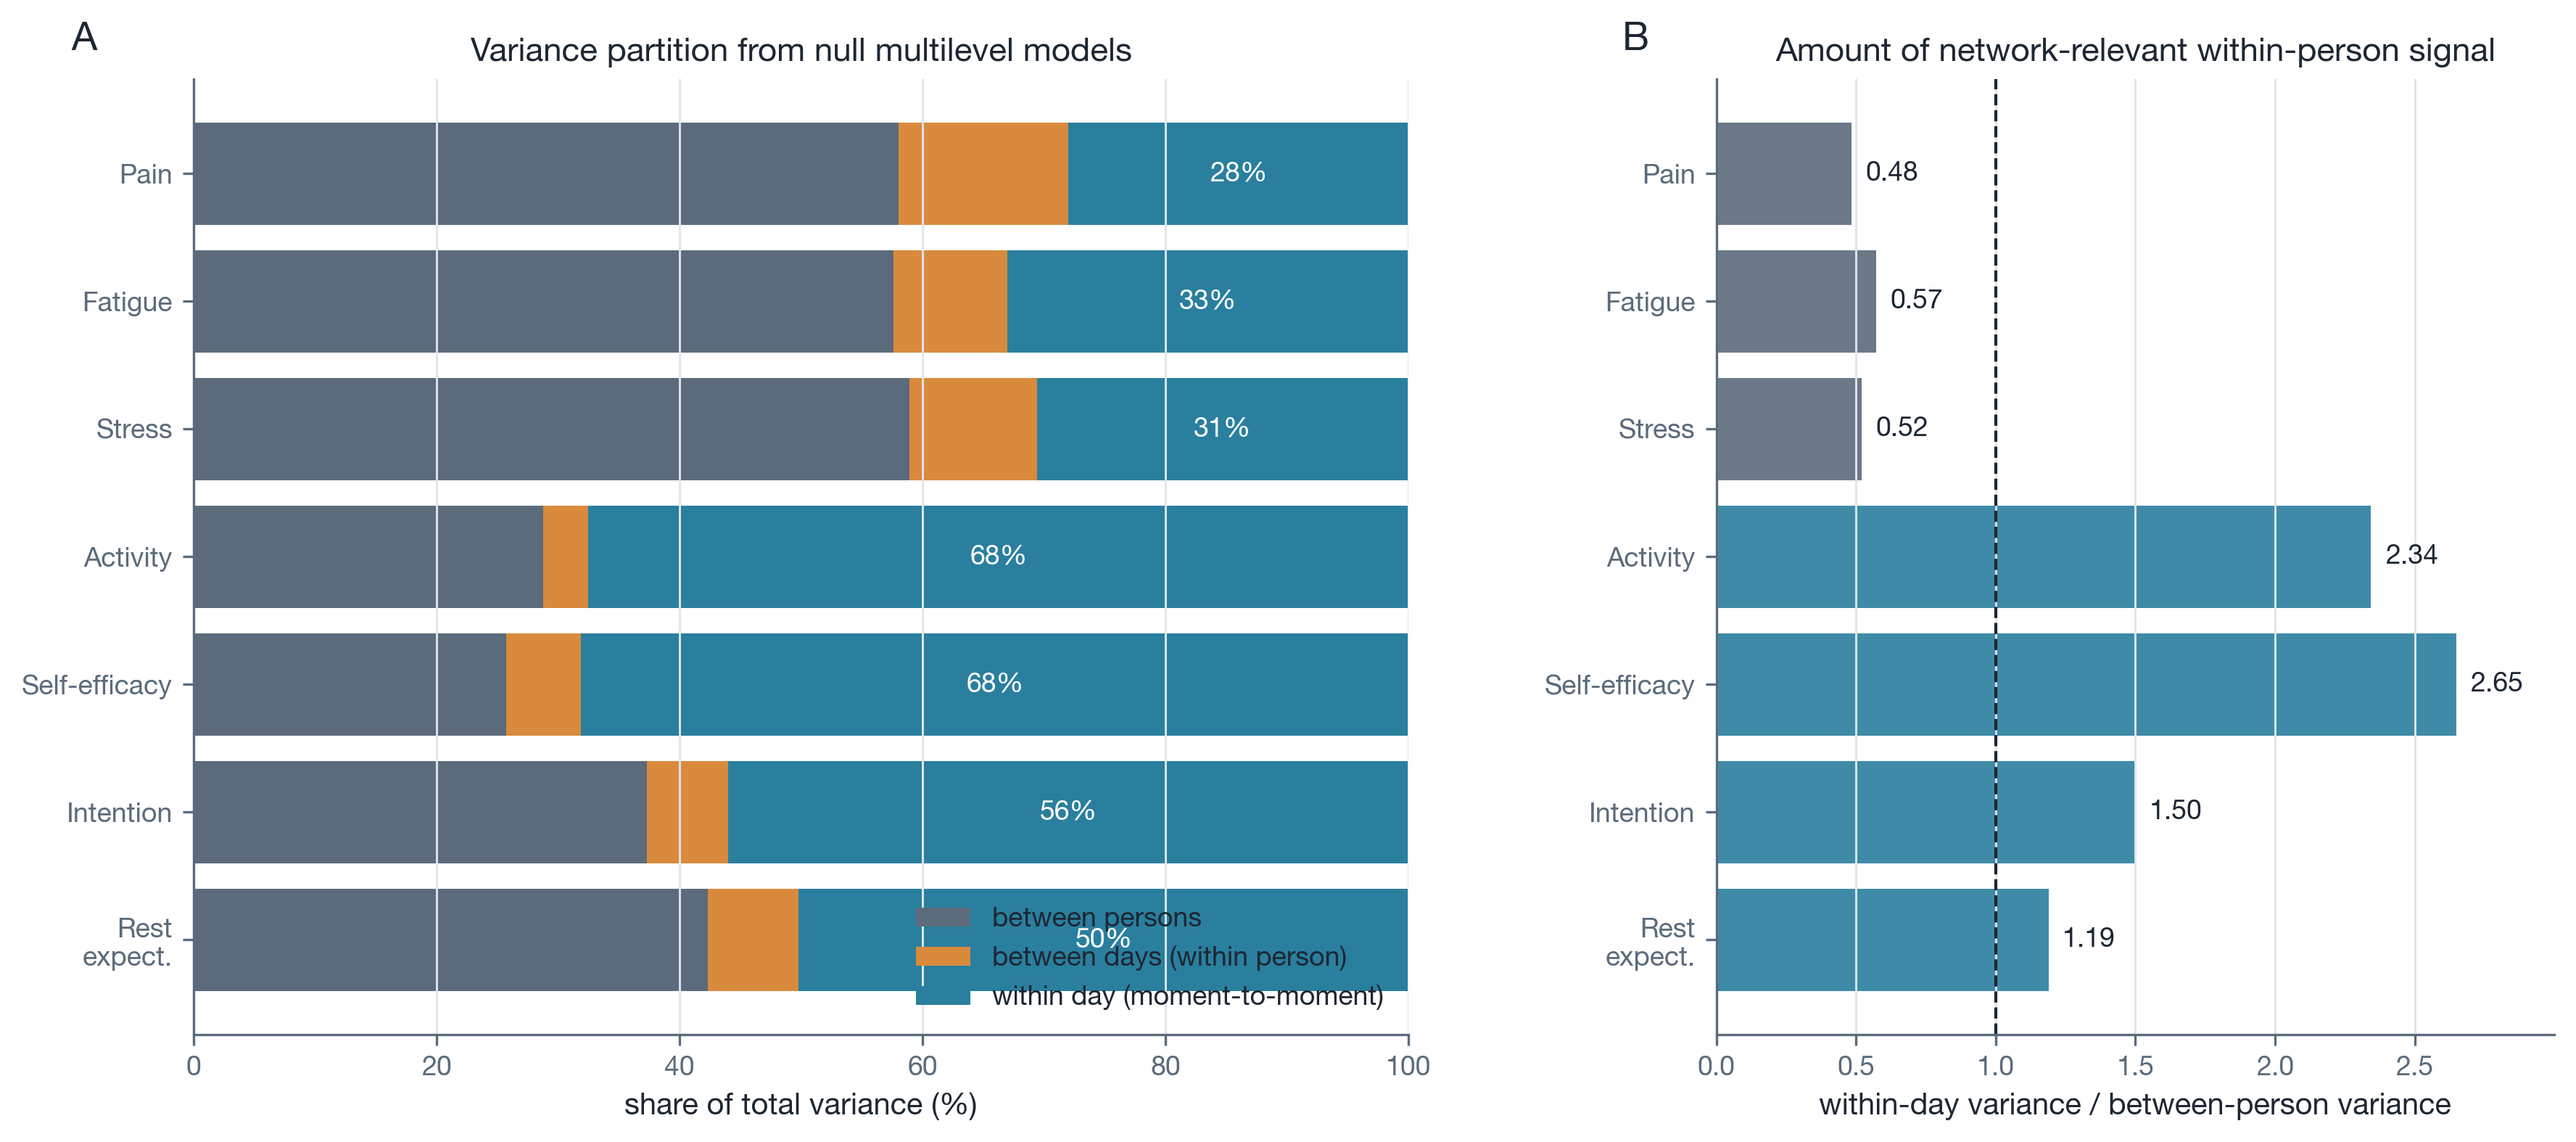
\includegraphics[width=0.96\textwidth]{../assets/figures/main/MAIN_01_variance_decomposition.png}
\figurenote{Panel A partitions each momentary measure into between-person, between-day, and
within-day variance. Panel B shows the within-day to between-person variance ratio, with
values above 1 indicating more moment-to-moment than between-person signal.}
\end{figure}

\begin{table}[H]
\raggedright
\caption{Momentary measures: descriptive statistics and variance partition.}
\label{tab:emadesc}
\footnotesize
\begingroup
\setlength{\tabcolsep}{4pt}
\renewcommand{\arraystretch}{1.08}
\noindent
\begin{tabular*}{\textwidth}{@{\extracolsep{\fill}}lcccccc@{}}
\toprule
Measure & $n$ obs & Mean & SD & \% miss. & ICC & Within-day var. \\
\midrule
Pain & 1497 & 5.64 & 2.06 & 21.0 & 0.58 & 0.28 \\
Fatigue & 1495 & 5.8 & 2.37 & 21.1 & 0.58 & 0.33 \\
Stress & 1492 & 3.16 & 2.29 & 21.2 & 0.59 & 0.31 \\
Activity (log) & 1757 & -3.63 & 0.71 & 7.2 & 0.29 & 0.68 \\
Self-efficacy & 1484 & 3.47 & 0.97 & 21.6 & 0.26 & 0.68 \\
Intention & 1483 & 3.62 & 1.01 & 21.7 & 0.38 & 0.56 \\
Rest-expectancy & 1483 & 3.03 & 1.0 & 21.7 & 0.43 & 0.5 \\
\bottomrule
\end{tabular*}
\par\vspace{3pt}\noindent\parbox{\textwidth}{\footnotesize\textit{Note.} ICC = intraclass correlation, the between-person share. Within-day var. is the moment-to-moment variance share available to the lag-1 network.}
\endgroup
\end{table}


\subsection{RQ1: Momentary networks}
\Cref{fig:networks} shows the temporal, contemporaneous, and between-person networks, and
\Cref{tab:temporal} reports the temporal fixed effects, which are repeated in
\Cref{tab:sup-temporal} for supplementary reference. In the temporal network, all four
core states were positively self-persistent (pain to pain $b=.364$, $SE=.053$, $p<.001$;
fatigue to fatigue $b=.285$, $SE=.042$, $p<.001$; stress to stress $b=.333$, $SE=.046$,
$p<.001$; activity to activity $b=.159$, $SE=.055$, $p=.004$). Two cross-lagged effects were
statistically significant at the group level: higher activity predicted lower subsequent
fatigue ($b=-.131$, $SE=.054$, $p=.015$, bootstrap 95\% CI $[-.247, -.038]$), and higher
stress predicted higher subsequent pain ($b=.081$, $SE=.036$, $p=.027$, bootstrap 95\% CI
$[.017, .150]$). The group-level symptom-to-activity paths were not statistically
significant: pain to activity ($b=-.004$, $SE=.050$, $p=.936$), fatigue to activity
($b=-.059$, $SE=.049$, $p=.235$), and stress to activity ($b=.065$, $SE=.049$, $p=.183$).
The contemporaneous network showed positive residual partial correlations among pain,
fatigue, and stress (pain-fatigue $r=.373$, $p<.001$; pain-stress $r=.190$, $p<.001$;
fatigue-stress $r=.109$, $p=.007$). The between-person network was dominated by a
pain-fatigue partial correlation ($r=.716$, $p<.001$).

\begin{figure}[htbp]
\raggedright
\caption{Group-level momentary networks from multilevel VAR.}
\label{fig:networks}
\noindent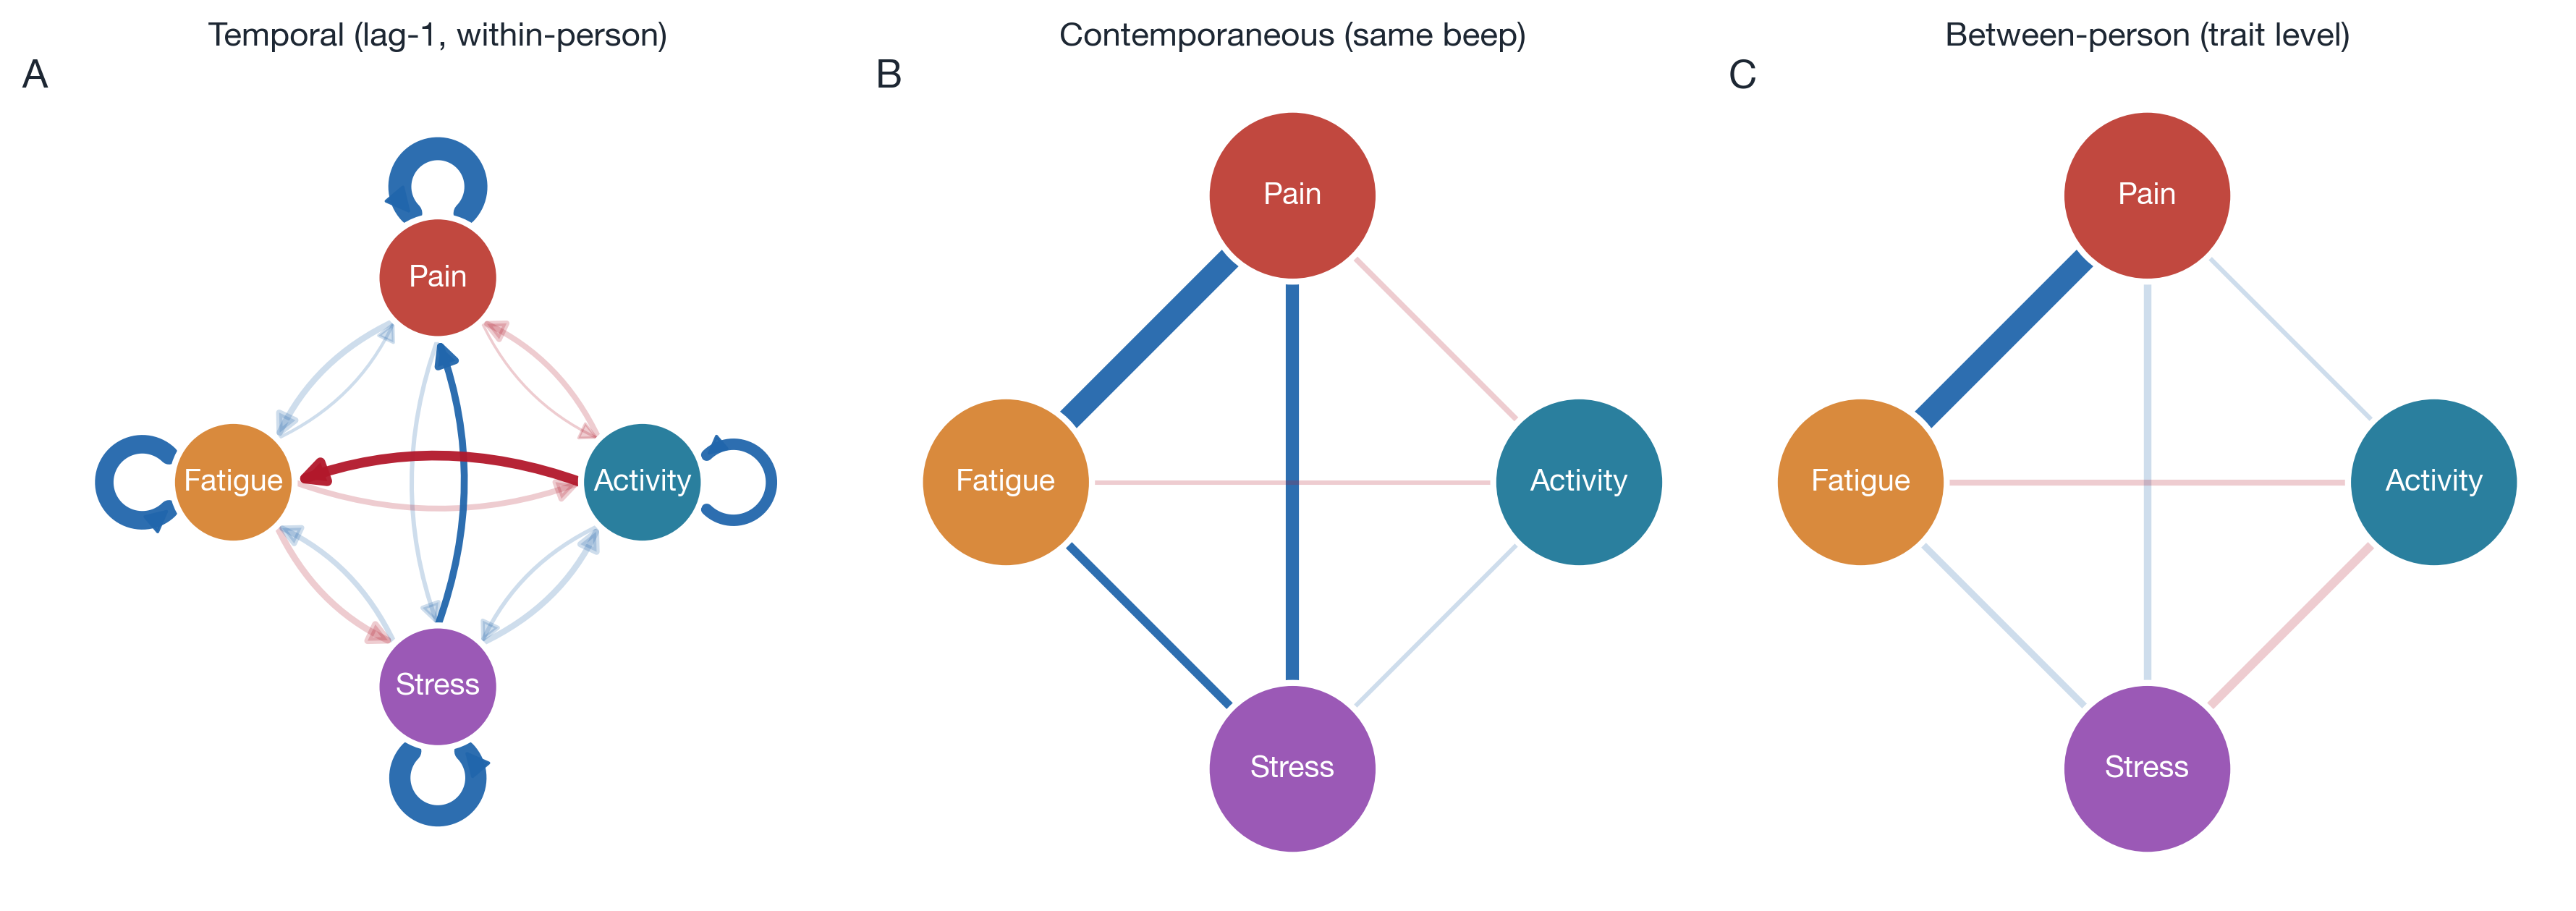
\includegraphics[width=0.96\textwidth]{../assets/figures/main/MAIN_02_mlvar_networks.png}
\figurenote{Panel A shows the directed temporal network within day. Panel B shows the
contemporaneous network at the same prompt. Panel C shows the between-person network. Blue
edges are positive, red edges are negative, edge width scales with strength, and faded edges
are not statistically significant.}
\end{figure}

\input{../assets/tables/main/MAIN_03_mlvar_temporal_effects}

\subsection{Individual heterogeneity and idiographic feasibility}
The group-level symptom-to-activity effects were close to zero, but per-person coefficients
varied widely. The unregularized per-person pain-to-activity coefficient ranged from $-.68$
to $.54$ across participants, and the displayed activity-related couplings showed both
negative and positive individual coefficients (\Cref{fig:heterogeneity}, Panels A and B).
The individual estimates were nonetheless imprecise: only 3 of the 33 per-person
pain-to-activity coefficients had a 95\% confidence interval that excluded zero
(\Cref{fig:heterogeneity}, Panel C), indicating that any single participant's network was
under-determined at a median of 44 observations. This between-person heterogeneity was also
structured rather than uniform, with the standard deviation of the per-person lag-1
coefficients largest for the activity-involving paths (\Cref{fig:heterogeneity}, Panel D). Fully separate individual
networks were correspondingly sparse: regularized graphicalVAR selected a median of 0 temporal
edges per person, and 16 of 30 fitted participants had no selected temporal edge
(\Cref{sfig:feasibility}). S-GIMME recovered the four autoregressive paths as
group-level paths, no group-level cross-variable path, and a weak subgroup structure with two
small groups and 14 singletons (\Cref{sfig:sgimme}). The six-node extension that added
momentary self-efficacy and intention left the core four-node temporal edges almost
unchanged ($r=.999$ between the 16 core coefficients), and the seven-node extension that
also added rest-favouring outcome expectancy did likewise ($r=.998$; \Cref{sfig:extended}).

\begin{figure}[htbp]
\raggedright
\caption{Group-level temporal effects and individual heterogeneity.}
\label{fig:heterogeneity}
\noindent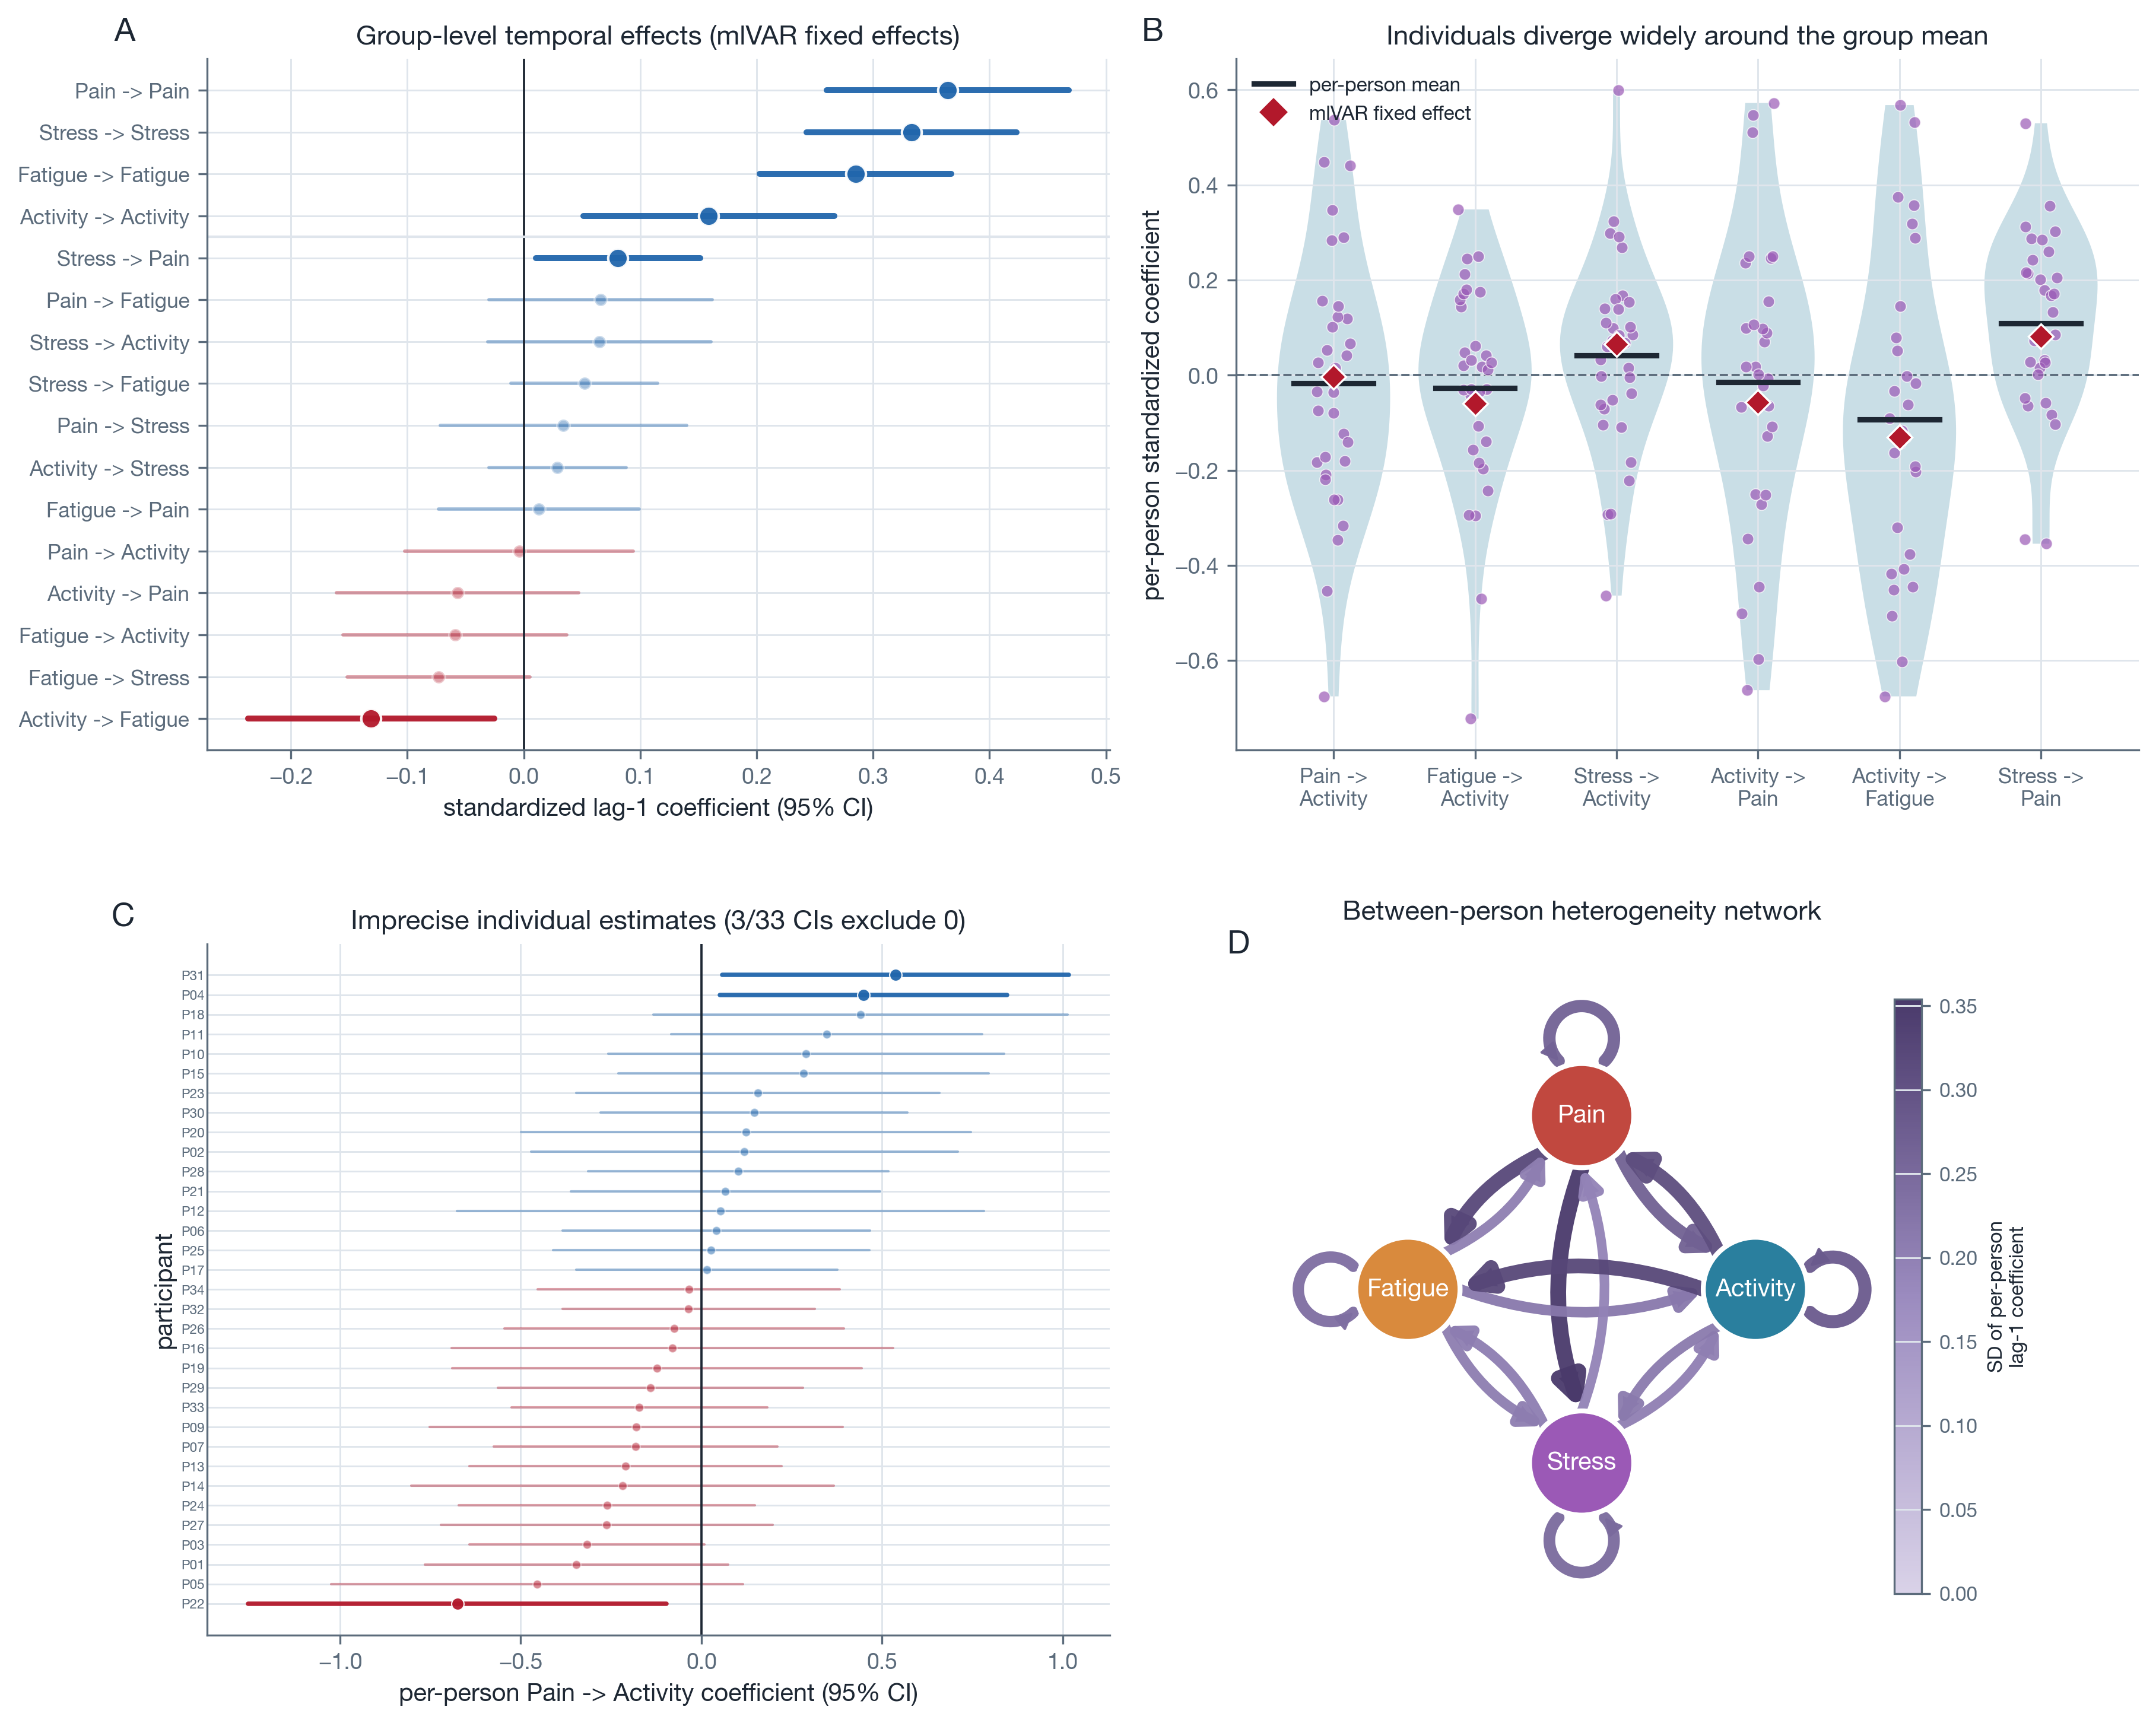
\includegraphics[width=0.96\textwidth]{../assets/figures/main/MAIN_03_temporal_effects_heterogeneity.png}
\figurenote{Panel A shows mlVAR fixed-effect estimates with 95\% confidence intervals. Panel B
shows the distribution of per-person standardized coefficients for the symptom-to-activity,
activity-to-symptom, and stress-to-pain couplings, with the per-person mean and the mlVAR
fixed effect marked so that the small group mean and the wide individual spread are
comparable. Panel C shows each participant's unregularized pain-to-activity estimate with its
95\% confidence interval, sorted, illustrating that individual estimates are imprecise at this
series length. Panel D shows the between-person heterogeneity network, in which the width and
colour intensity of each edge both scale with the standard deviation of the per-person lag-1
coefficient for that path.}
\end{figure}

\subsection{RQ2: Activity-pattern subgroups and the network link}
The POAM-P dominant-pattern typology produced three subgroups: overdoing ($n=12$), avoidance
($n=10$), and pacing ($n=9$). Data-driven clustering favoured a weakly separated two-cluster
solution (silhouette = .31), so the dominant-pattern typology was retained as the primary
interpretable grouping. The individual pain-to-activity coupling differed across dominant
patterns (Kruskal-Wallis $H=6.46$, $p=.040$; permutation $p=.037$): avoiders showed negative
mean coupling ($M=-.153$), overdoers were near zero ($M=.025$), and pacers showed positive
mean coupling ($M=.125$; \Cref{fig:poamp}, \Cref{tab:link}). The pain-to-activity coupling
was also correlated with the continuous POAM-P avoidance score (Spearman $\rho=-.394$,
asymptotic $p=.031$, permutation $p=.033$). This association was specific to avoidance rather
than to overdoing ($\rho=.109$, $p=.567$) or pacing ($\rho=-.131$, $p=.491$; \Cref{fig:poamp},
Panels C to E). In an exploratory scan of every coupling against every subscale, the
activity-to-fatigue coupling was positively associated with the overdoing score (Spearman
$\rho=.514$, $p=.006$, uncorrected), although its three-group comparison was not significant
(\Cref{fig:poamp}, Panel F). Other activity-related couplings did not differ significantly
across dominant patterns (all permutation $p \geq .119$). When the pain-to-activity coupling
was regressed jointly on all three standardized POAM-P subscales, the model was not
statistically significant and explained little variance ($R^2=.11$, adjusted $R^2=.01$,
overall $F$ $p=.372$; avoidance $\beta=-.093$, $p=.128$), consistent with the limited power of
a three-predictor model at $N=30$. Clustering participants by their dynamic structure did not
yield interpretable subgroups either, because S-GIMME returned only two small groups and 14
singletons (modularity = .27), so the data-driven network subgroups could not be meaningfully
aligned with the POAM-P patterns. The RQ2 results are therefore exploratory and
hypothesis-generating.

\begin{figure}[htbp]
\raggedright
\caption{POAM-P activity-pattern subgroups and momentary dynamics.}
\label{fig:poamp}
\noindent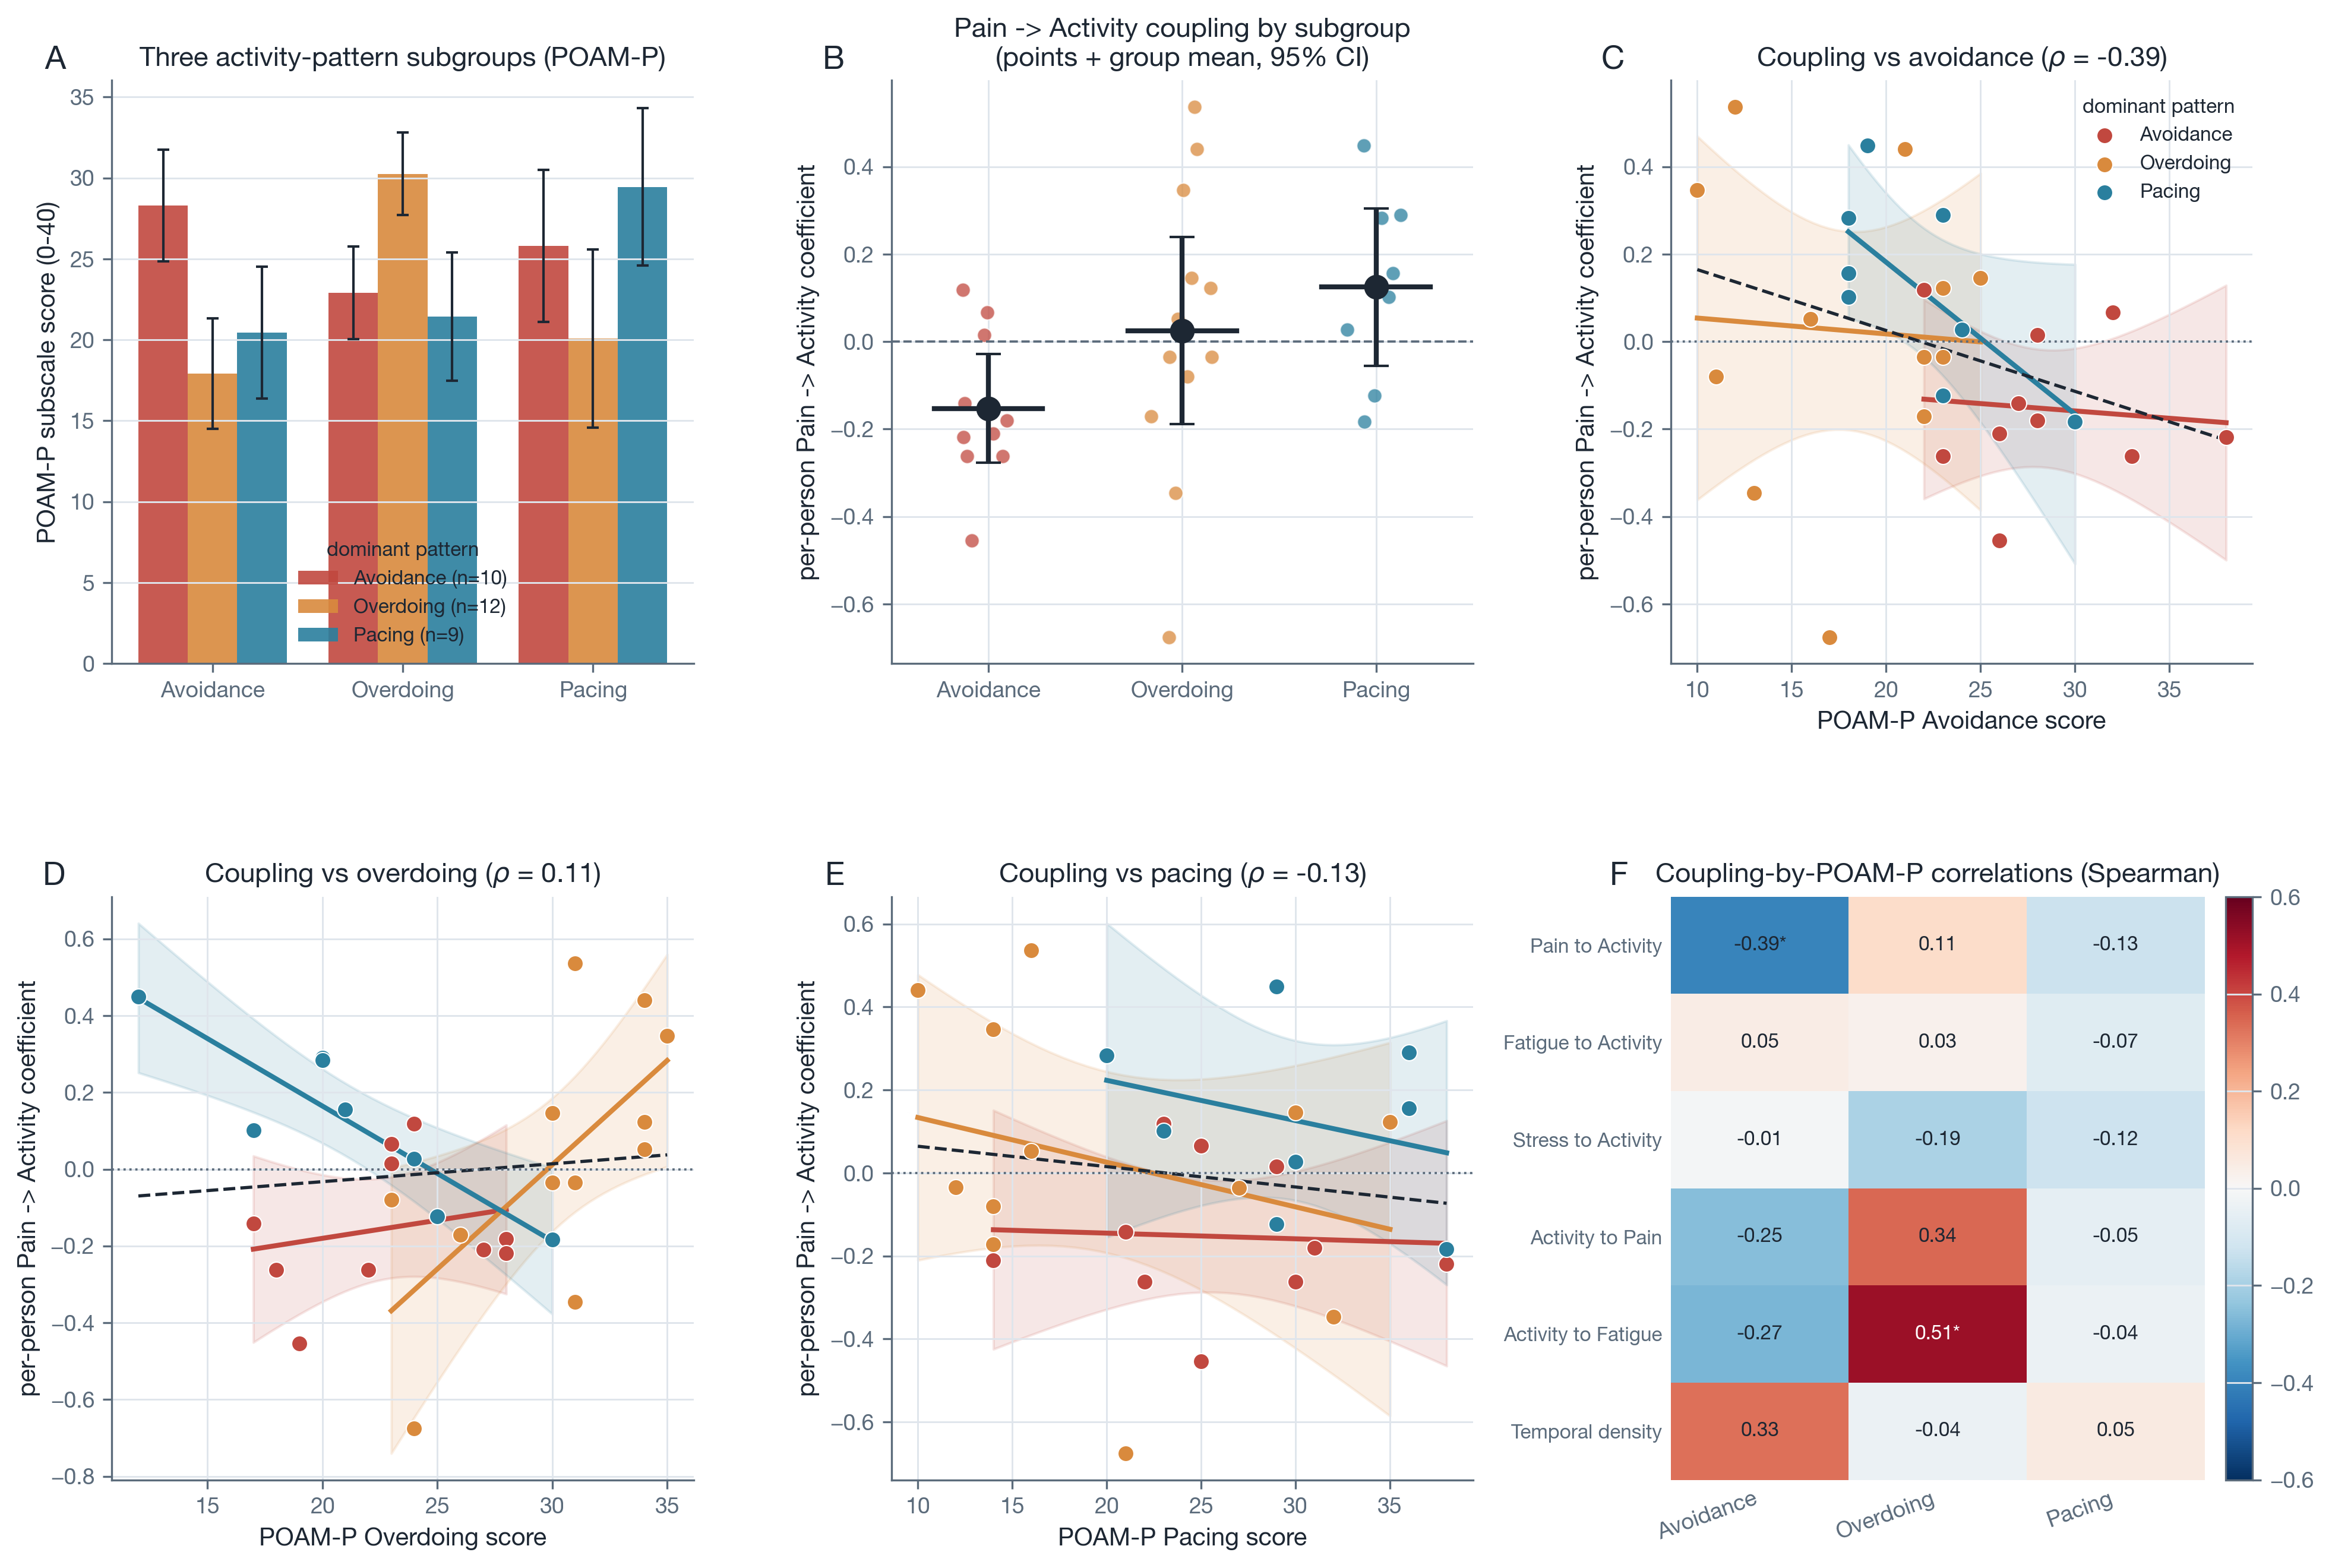
\includegraphics[width=0.96\textwidth]{../assets/figures/main/MAIN_04_poamp_subgroups_link.png}
\figurenote{Panel A shows the POAM-P subgroup profiles with 95\% confidence intervals. Panel B
shows the per-person pain-to-activity coupling by dominant pattern, with subgroup means and
95\% confidence intervals. Panels C, D, and E show the association between the per-person
pain-to-activity coupling and the POAM-P avoidance, overdoing, and pacing scores respectively,
each with subgroup-specific fits and an overall reference trend. Panel F shows the Spearman
correlations between each temporal coupling and the three POAM-P subscales, with an asterisk
marking $p<.05$.}
\end{figure}

\begin{table}[H]
\raggedright
\caption{Individual network parameters by POAM-P dominant pattern (exploratory).}
\label{tab:link}
\footnotesize
\begingroup
\setlength{\tabcolsep}{4pt}
\renewcommand{\arraystretch}{1.08}
\noindent
\begin{tabular*}{\textwidth}{@{\extracolsep{\fill}}lccccc@{}}
\toprule
Coupling & Avoidance & Overdoing & Pacing & KW $H$ & $p$ \\
\midrule
Pain $\rightarrow$ Activity & -0.153 & 0.025 & 0.125 & 6.46 & .040 \\
Fatigue $\rightarrow$ Activity & 0.026 & -0.036 & -0.074 & 0.38 & .827 \\
Stress $\rightarrow$ Activity & 0.084 & 0.016 & -0.005 & 1.646 & .439 \\
Activity $\rightarrow$ Pain & -0.024 & 0.064 & -0.169 & 4.149 & .126 \\
Activity $\rightarrow$ Fatigue & -0.146 & 0.055 & -0.238 & 4.215 & .122 \\
Temporal density & 0.14 & 0.131 & 0.12 & 3.059 & .217 \\
\bottomrule
\end{tabular*}
\par\vspace{3pt}\noindent\parbox{\textwidth}{\footnotesize\textit{Note.} Mean per-person standardized VAR(1) coefficients by subgroup (Avoidance $n=10$, Overdoing $n=12$, Pacing $n=9$). KW = Kruskal-Wallis test across subgroups. Exploratory ($N=30$, uncorrected).}
\endgroup
\end{table}


\subsection{Robustness}
The temporal network was stable across sensitivity analyses. The full set of 16 temporal
coefficients reproduced under within-person detrending ($r=.968$ with the primary model),
a stricter compliance threshold ($r=.984$), raw and square-root activity scales ($r=.997$ and
$r=.999$), exclusion of could-not-move prompts ($r=.982$), the six-node specification
($r=.999$), and the seven-node specification ($r=.998$), with no sign changes
(\Cref{sfig:robustness}, \Cref{tab:agreement}). In
leave-one-participant-out refits, all cross-lagged edges retained their sign across all
34 refits. In the person-level bootstrap, the two significant cross-lagged effects had 95\%
intervals that excluded zero: activity to fatigue ($[-.247, -.038]$) and stress to pain
($[.017, .150]$; \Cref{tab:robust}). Residual diagnostics showed near-zero mean
within-person lag-1 residual autocorrelation, approximately homogeneous residual variance,
and the expected mild non-normality for bounded rating scales (\Cref{sfig:diagnostics}).
Everyday context summaries showed that most prompts occurred at home and that objective
activity was higher away from home. Alone-versus-accompanied GEE contrasts for pain,
fatigue, and stress were not statistically significant (pain $b=.140$, $p=.266$; fatigue
$b=.085$, $p=.399$; stress $b=.180$, $p=.114$; \Cref{sfig:context}). Group-level day-type
contrasts showed no weekday-weekend differences in the continuous momentary measures (all
$p \geq .184$), although participant-level reports of being alone were more frequent on
weekends than weekdays (median difference = 20.83 percentage points, Wilcoxon $p<.001$;
\Cref{sfig:daytype}).

\section{Discussion}
This study characterized how momentary pain, fatigue, and stress relate to objectively
measured physical activity within individuals with FM, and whether these dynamics differ by
baseline activity pattern. A multilevel vector autoregressive model served as the primary
analysis because the available series length did not support fully separate idiographic
networks. The findings are discussed below for each research question, followed by limitations
and directions for future work.

\subsection{Main findings}

\subsubsection{Momentary dynamics of pain, fatigue, stress, and activity (RQ1)}
At the group level, all four momentary states were strongly self-persistent, and two
cross-lagged couplings emerged: higher activity preceded lower fatigue, and higher stress
preceded higher pain. The autoregressive effects were moderate for pain ($b=.364$), fatigue
($b=.285$), and stress ($b=.333$), and smaller for activity ($b=.159$; all $p\leq .004$).
The activity-to-fatigue effect was negative ($b=-.131$, $SE=.054$, $p=.015$, bootstrap 95\%
CI $[-.247, -.038]$), which is consistent with the documented benefits of physical activity
in FM \citep{busch2007exercise,geneen2017physical} and runs counter to the expectation that
movement inevitably aggravates symptoms. The stress-to-pain effect was positive ($b=.081$,
$SE=.036$, $p=.027$, bootstrap 95\% CI $[.017, .150]$), aligning with
psychoneuroendocrine accounts that link sustained stress to the amplification of pain
\citep{hannibal2014chronic} and with the affective emphasis of contemporary
fear-avoidance models \citep{crombez2012fear}.

The central RQ1 result, however, concerns heterogeneity rather than the average. The
group-level symptom-to-activity paths were close to zero, yet the unregularized per-person
pain-to-activity coefficient ranged from $-.68$ to $.54$ while the fixed effect was
essentially absent ($b=-.004$, $SE=.050$, $p=.936$). A single average effect therefore
obscured opposite individual dynamics, a concrete instance of the group-to-individual
non-generalizability that motivates within-person modelling
\citep{fisher2018lack,molenaar2004manifesto}. The feasibility analyses then addressed whether
those individual dynamics can be estimated person by person. They cannot at this series
length: only 3 of 33 individual pain-to-activity confidence intervals excluded zero,
regularized graphicalVAR selected a median of 0 temporal edges per person, and S-GIMME
recovered no group-level cross-variable path and no interpretable subgroup structure. These
findings are consistent with the series length lying well below the length usually
recommended for idiographic estimation \citep{beltz2016bridging}.
Partial pooling through mlVAR is therefore the appropriate level of analysis, because it
retains the group structure while expressing individual differences as random effects
\citep{epskamp2018gaussian,bringmann2013network}. The six-node extension further indicated that
momentary self-efficacy and intention can be incorporated without distorting the core temporal
structure ($r=.999$ for the 16 core edges); the seven-node extension that added
rest-favouring outcome expectancy provided the same substantive check ($r=.998$). The substantial
within-day variance in these motivational states marks them as promising additional nodes
once longer series are available \citep{schwarzer2008modeling,maes2022variability}.

\subsubsection{Activity patterns and individual differences (RQ2)}
The per-person pain-to-activity coupling differed by baseline activity pattern: participants
with a dominant avoidance pattern tended to reduce activity as pain rose, whereas pacers showed
the opposite tendency (Kruskal-Wallis $H=6.46$, $p=.040$; permutation $p=.037$; avoidance
$M=-.153$, overdoing $M=.025$, pacing $M=.125$). The association was specific to avoidance:
the continuous POAM-P avoidance score correlated with the pain-to-activity coupling
($\rho=-.394$, asymptotic $p=.031$, permutation $p=.033$), whereas overdoing and pacing did
not ($\rho=.109$ and $-.131$, respectively). This patterning is consistent with the
fear-avoidance model \citep{vlaeyen2000fear,leeuw2007fear} and with activity-pattern theory,
which distinguishes avoidance, overdoing, and pacing as habitual ways of regulating activity
around pain \citep{cane2013pain,andrews2012activity}. An exploratory signal additionally
linked the activity-to-fatigue coupling to the overdoing pattern (Spearman $\rho=.514$,
$p=.006$, uncorrected), consistent with a boom-and-bust style of overactivity
\citep{nielson2013activity}. These RQ2 results are nonetheless hypothesis-generating rather
than confirmatory: the joint regression of the pain-to-activity coupling on all three
subscales was underpowered and non-significant ($R^2=.11$, adjusted $R^2=.01$, overall
$F$ $p=.372$), and the data-driven network clustering did not yield interpretable subgroups.
Larger samples are needed before the activity-pattern moderation can be established
\citep{wright2020personalized}.

\subsection{Limitations}
Several limitations qualify these conclusions. First, and most consequentially, the median of
44 completed prompts per person falls well below the 100 to 120 observations commonly
recommended for stable individual networks. The partial-pooling model therefore provides the
most defensible level of analysis for these data, but it cannot fully recover each person's
dynamic system \citep{beltz2016bridging}.

Second, the sample of 34 participants, of whom 31 had POAM-P data, produced small
activity-pattern subgroups. The RQ2 analyses are therefore exploratory, and subgroup means
are vulnerable to individual influential observations even though permutation tests supported
the dominant-pattern finding.

Third, the temporal resolution was coarse and unequal. Four semi-random prompts per day made
lag-1 an adjacent within-day contrast separated by several variable hours, and no lag was
carried across the overnight interval. Some pain-activity processes may unfold faster than
this design can observe, whereas other behavioural adjustments may require longer than a
single prompt interval \citep{hamaker2017no}.

Fourth, the analysis was observational. Pain, fatigue, stress, motivation, social context, and
activity were not manipulated, and the variables can influence one another through unmeasured
time-varying causes. The temporal edges should therefore be interpreted as predictive
within-person associations rather than causal effects \citep{rohrer2018thinking}.

Fifth, the heterogeneity estimates involve a trade-off. The mlVAR random effects borrow
strength across participants but shrink person-specific effects toward the group mean,
whereas the unregularized per-person coefficients preserve the observed spread but are noisy
at this series length. The wide pain-to-activity range is clinically informative, but the
individual coefficients should not be overinterpreted as precise person-level parameters.

Sixth, momentary symptoms were self-reported and may be affected by reporting biases or
reactivity to repeated assessment \citep{shiffman2008ecological}. Wrist accelerometry
captured movement volume but not posture, activity type, perceived exertion, or the personal
meaning of the activity, and roughly 13\% of answered prompts occurred in situations where
movement was reported as impossible.

Seventh, missingness remains a limitation despite the diagnostics. Objective-activity
missingness was not predicted by pain, fatigue, or stress, and the imputation benchmark
supported the available-case decision, but data missing not at random cannot be ruled out.
All participants were women from one FM cohort, so replication is needed before generalizing
to men with FM, other chronic pain conditions, or more diverse clinical settings
\citep{hauser2015fibromyalgia}.

\subsection{Future directions}
Future EMA studies should use longer and denser protocols when the aim is idiographic
network estimation. Protocols approaching at least 100 observations per participant would
support more stable person-specific networks, more credible data-driven subgrouping, and
better-powered tests of activity-pattern moderation \citep{wright2020personalized,
beltz2016bridging}.

Single-case experimental and N-of-1 designs are needed to move from prediction toward
mechanism. For example, activity pacing, graded activity, or stress-regulation components
could be experimentally varied to test whether changing a person's pain-to-activity coupling
also changes later activity or fatigue \citep{kwasnicka2020nof1,bentley2019realtime}.

The motivational and contextual node set should be expanded in designs with sufficient
series length. Self-efficacy, intention, and outcome expectancy showed enough within-person
variation to justify further study, and context variables such as location, social setting,
movement opportunity, and day type can help specify when a symptom-activity coupling is most
likely to occur \citep{schwarzer2008modeling,maes2022variability}.

Future work should also improve measurement of activity. Combining wrist accelerometry with
posture sensing, activity classification, ecological audio or location summaries, and lower
burden passive sensing could distinguish exercise, chores, commuting, and constrained
sedentary time more clearly while reducing missingness and participant burden.

Finally, replication in larger and more diverse samples should evaluate whether the
avoidance-linked pain-to-activity pattern is specific to FM or reflects a broader chronic
pain process. If replicated, person-specific coupling estimates and POAM-P profiles could be
used together to tailor physical-activity and pacing interventions in the spirit of precision
behaviour change \citep{kwasnicka2020nof1}.

\section{Conclusion}
This 14-day EMA and accelerometry study showed that daily pain, fatigue, stress, and activity
in FM are temporally structured but not well summarized by a single symptom-to-activity
average. Activity was followed by lower fatigue, stress was followed by higher pain, and the
average pain-to-activity path was near zero despite a wide spread of person-specific
coefficients that aligned with baseline avoidance. At this series length, fully separate
idiographic networks were too imprecise to support person-level inference, whereas
partial-pooling mlVAR preserved the group-level temporal structure while quantifying
heterogeneity. The findings therefore support within-person, activity-pattern-sensitive
models as a more useful basis for understanding, and eventually tailoring, physical activity
support in fibromyalgia.

\clearpage
\bibliographystyle{apalike}
\bibliography{references}

\clearpage
\renewcommand{\thefigure}{S\arabic{figure}}
\renewcommand{\thetable}{S\arabic{table}}
\setcounter{figure}{0}
\setcounter{table}{0}

\section*{Appendix}
\addcontentsline{toc}{section}{Appendix}
\subsection*{Supplementary Figures}
\addcontentsline{toc}{subsection}{Supplementary Figures}

\begin{figure}[H]
\raggedright
\caption{Design, compliance, and data quality.}
\label{sfig:design}
\noindent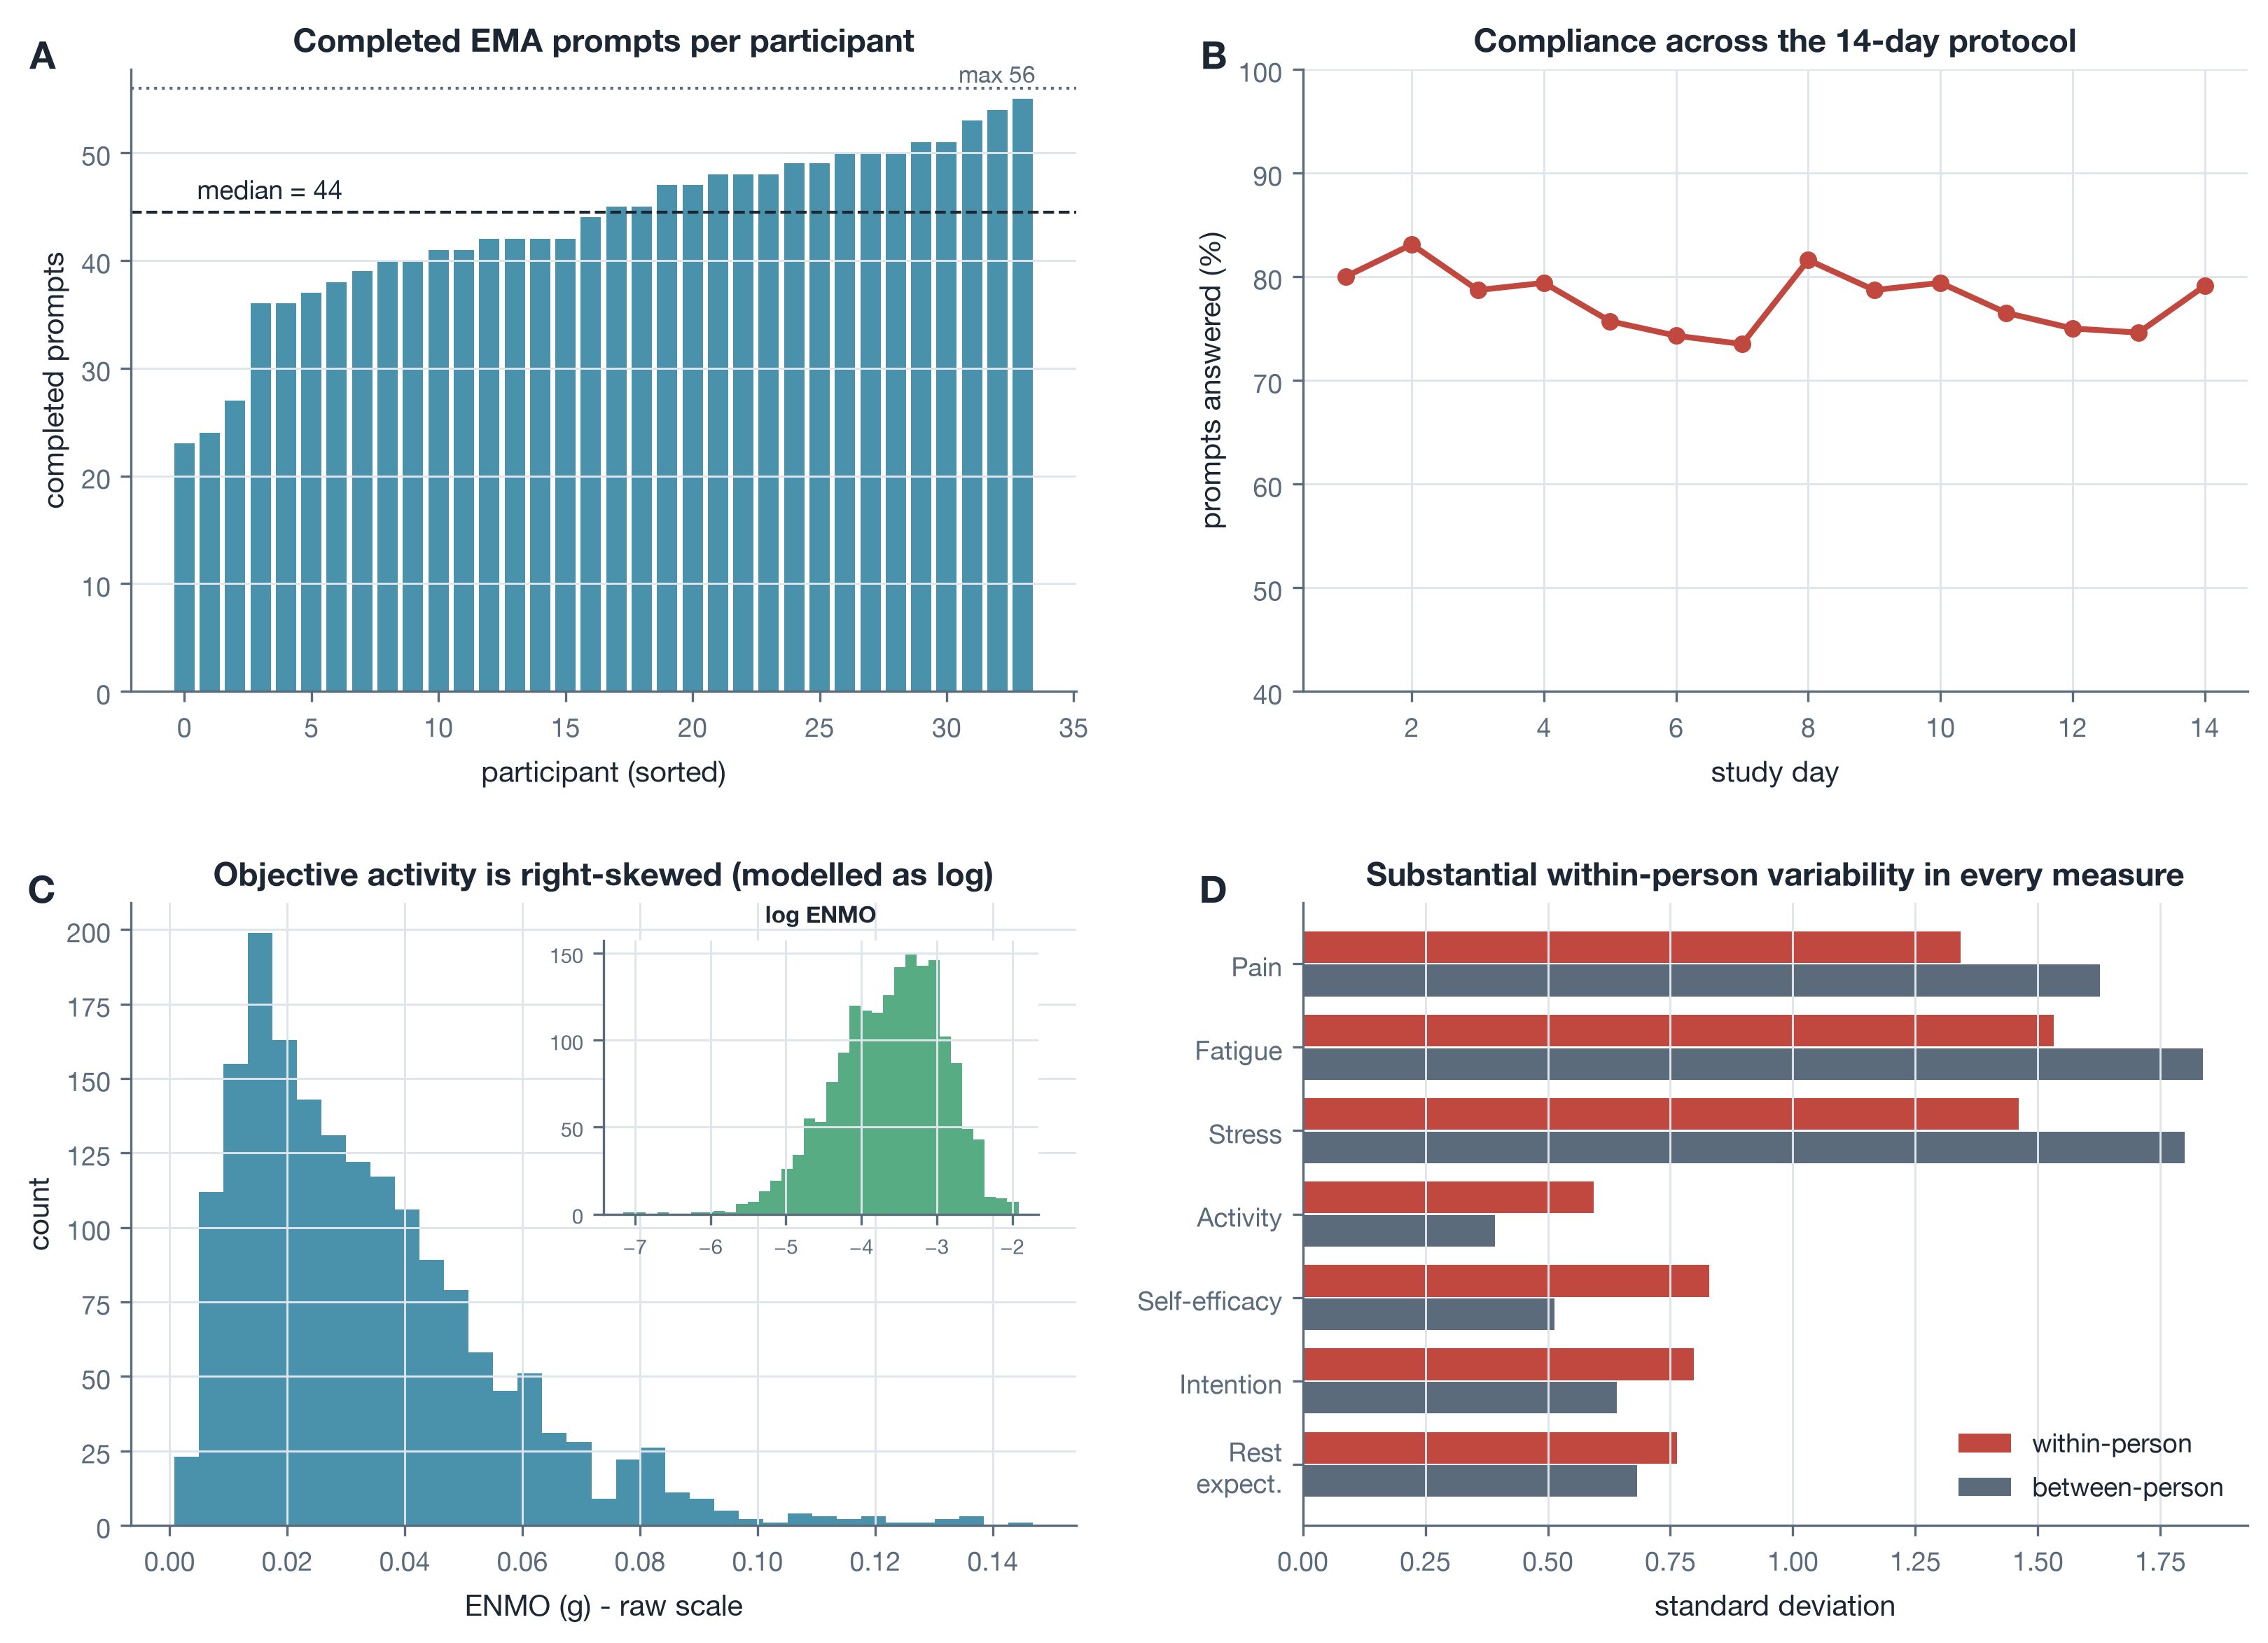
\includegraphics[width=0.92\textwidth]{../assets/figures/supplementary/SUP_01_design_compliance.png}
\figurenote{Panel A shows completed prompts per participant. Panel B shows compliance across
the 14-day protocol. Panel C shows the right-skewed ENMO distribution and the log-transformed
distribution used for modelling. Panel D compares within-person and between-person standard
deviations.}
\end{figure}

\begin{figure}[H]
\raggedright
\caption{EMA protocol timing audit.}
\label{sfig:timing}
\noindent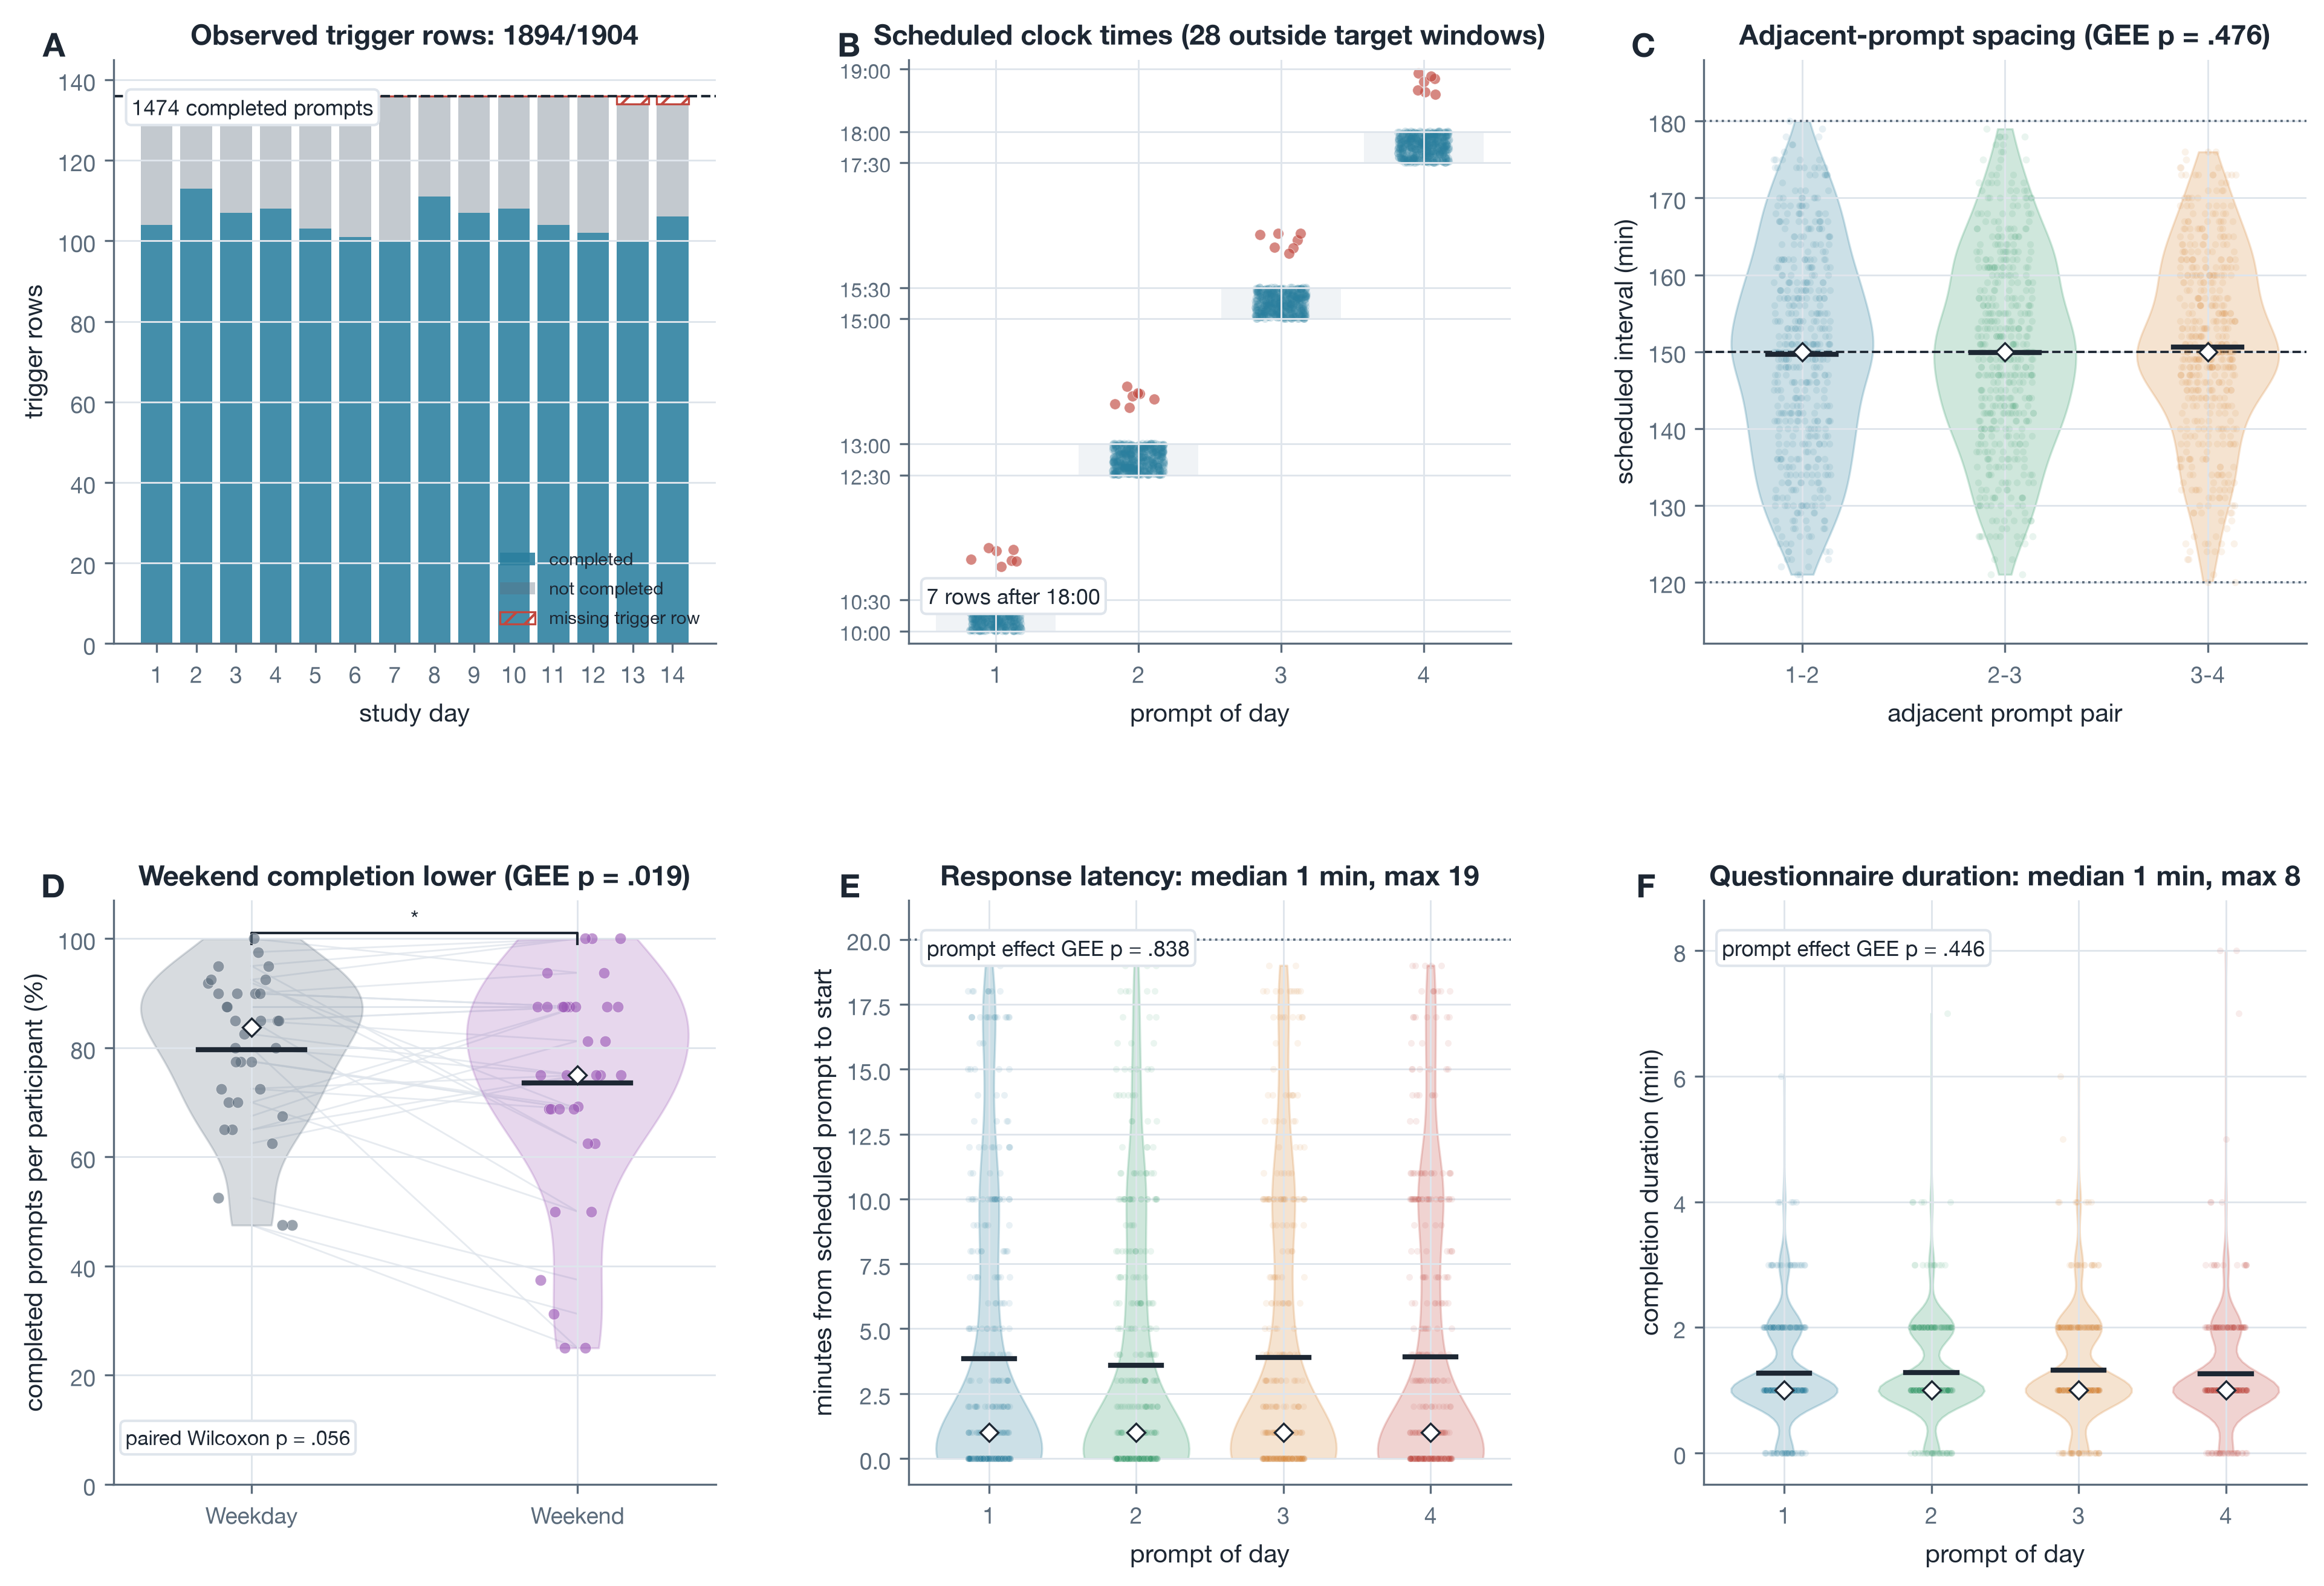
\includegraphics[width=0.96\textwidth]{../assets/figures/supplementary/SUP_02_ema_timing.png}
\figurenote{Panel A shows observed, completed, missed, and technically missing trigger rows
by study day. Panel B shows scheduled clock times by prompt of day; shaded bands mark the
target 30-minute windows. Panel C shows scheduled adjacent-prompt intervals, with reference
lines at 120, 150, and 180 minutes. Panel D compares weekday and weekend completion
percentages per participant; the significance bar uses a participant-clustered binomial GEE.
Panel E shows response latency from scheduled prompt to questionnaire start. Panel F shows
the time needed to complete the questionnaire.}
\end{figure}

\begin{figure}[H]
\raggedright
\caption{ENMO transformation and per-person stationarity.}
\label{sfig:stationarity}
\noindent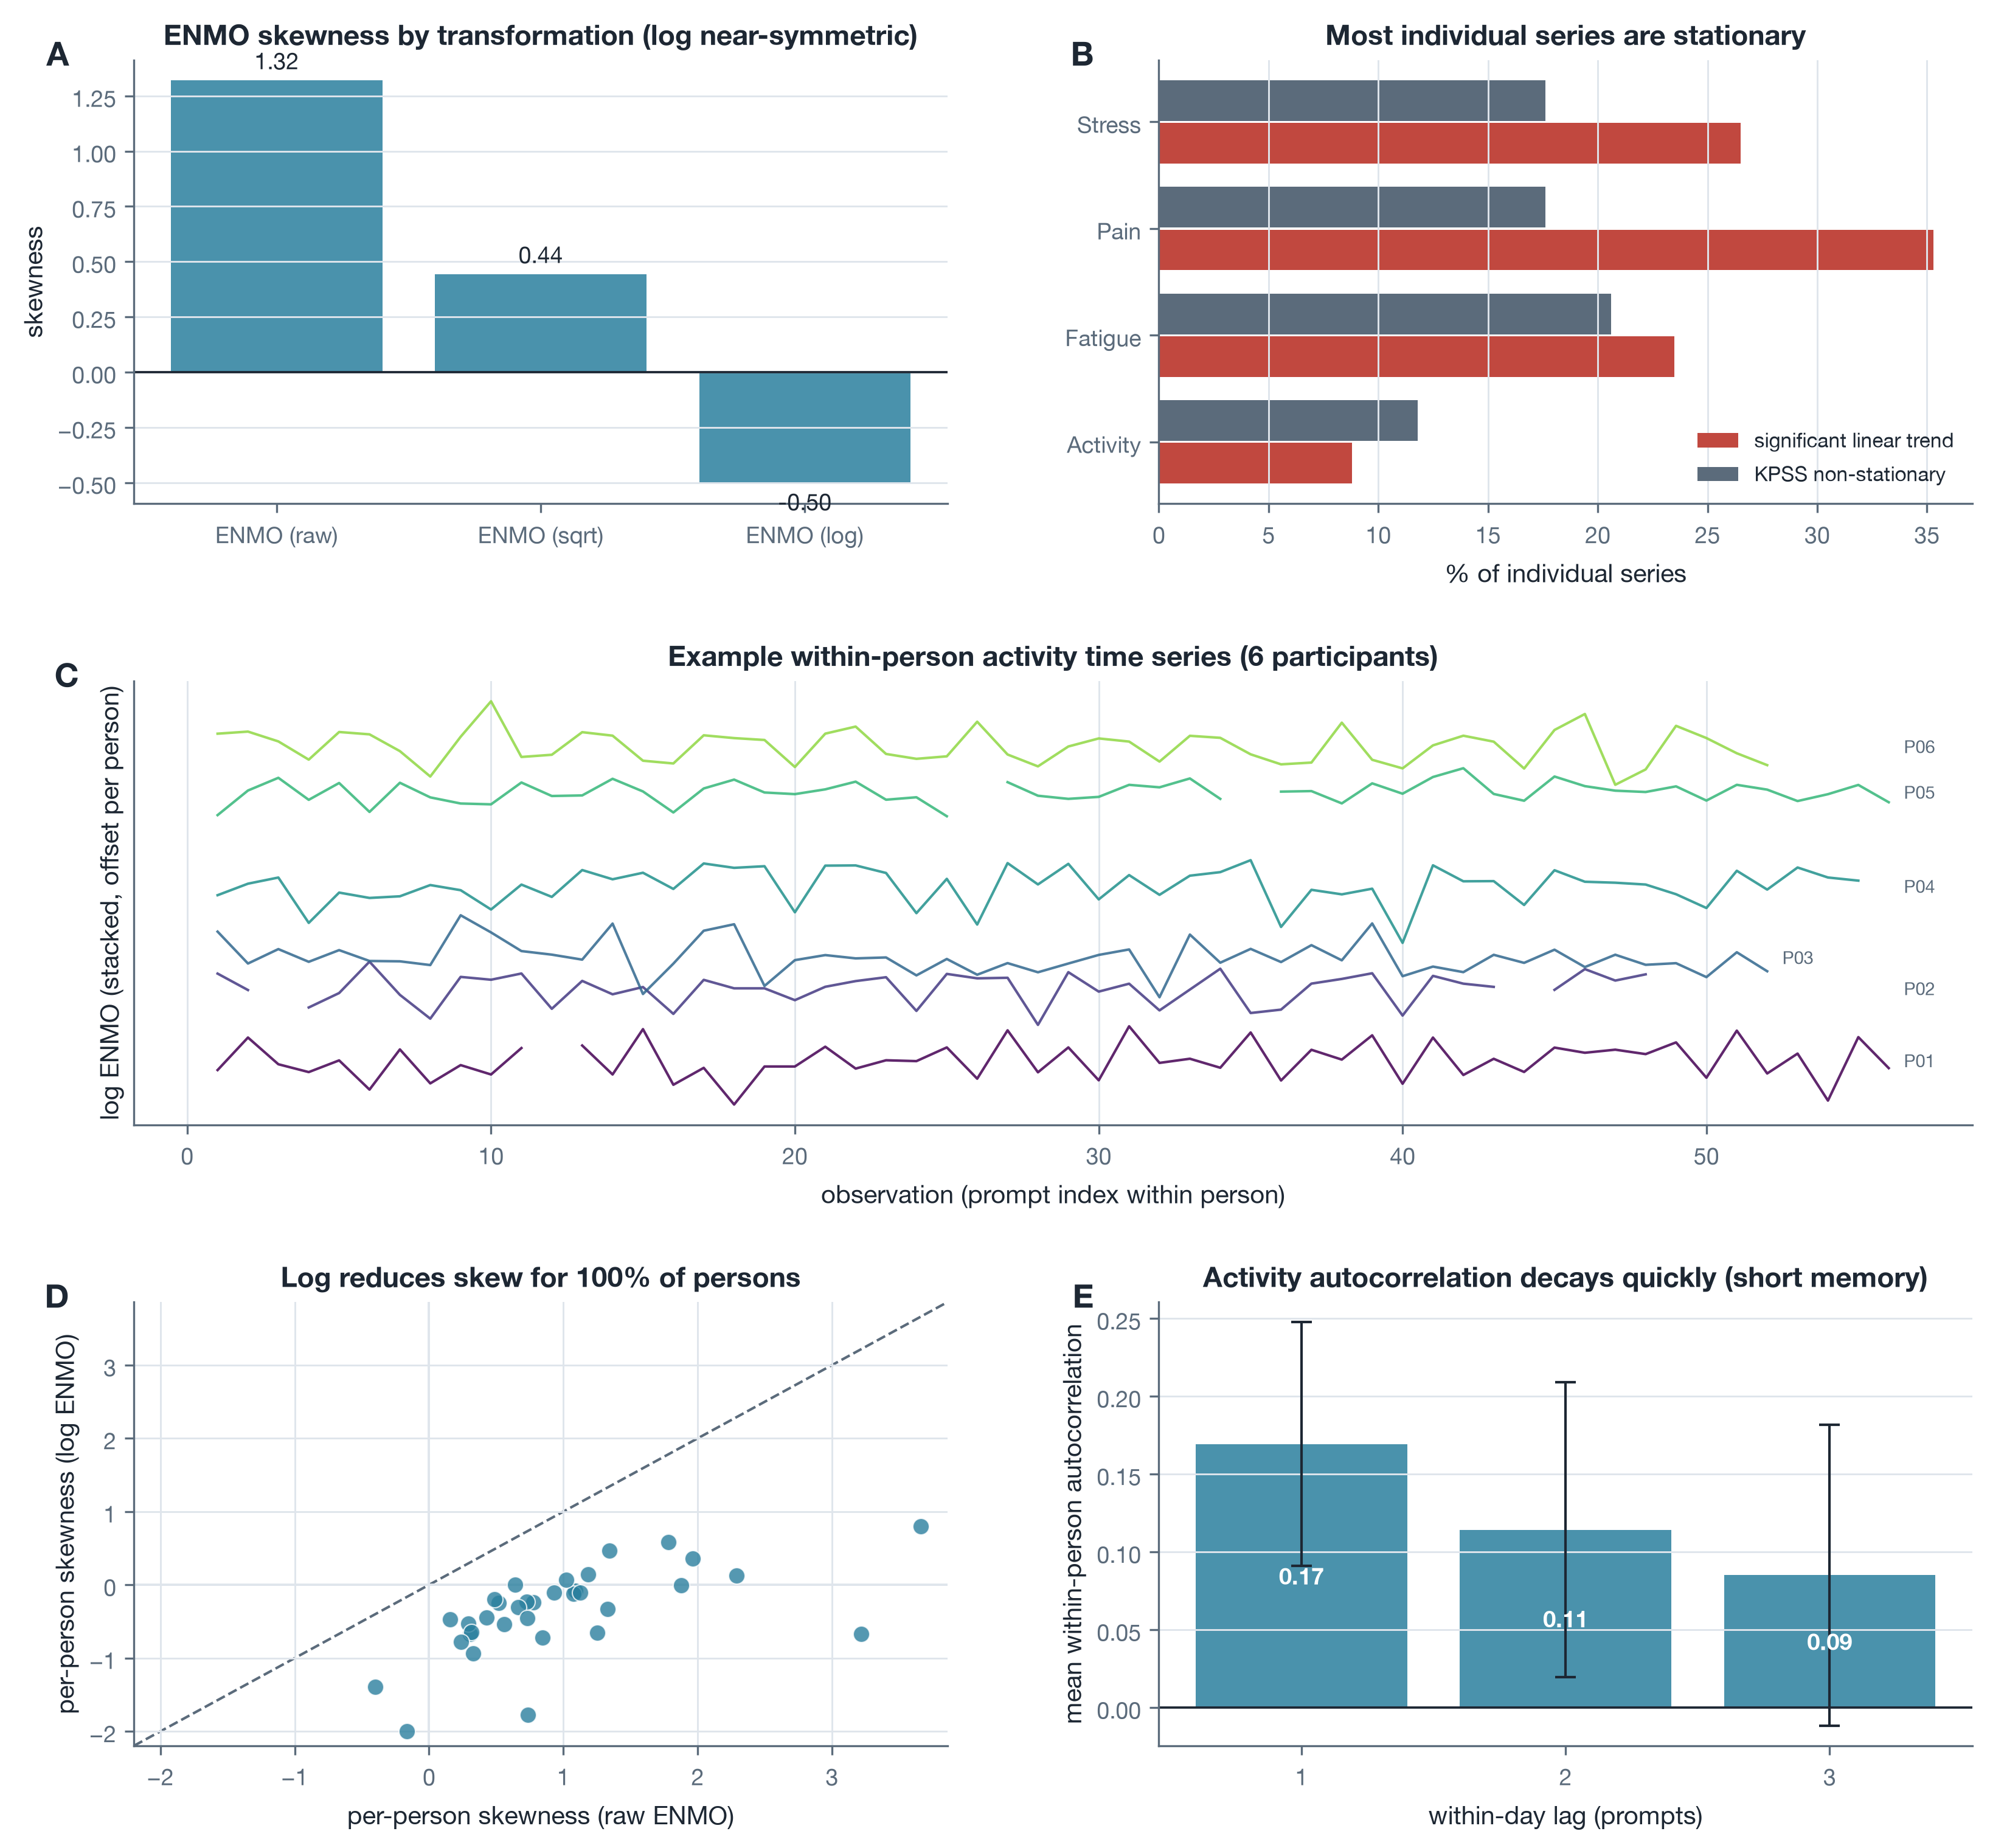
\includegraphics[width=0.92\textwidth]{../assets/figures/supplementary/SUP_03_stationarity_transform.png}
\figurenote{Panel A shows ENMO skewness under the raw, square-root, and log transformations.
Panel B shows the share of individual series flagged by a significant linear trend and by the
KPSS test. Panel C shows example within-person log-activity time series for six participants.
Panel D compares per-person skewness on the raw and log scales. Panel E shows the mean
within-person autocorrelation of log-activity at within-day lags one to three.}
\end{figure}

\begin{figure}[H]
\raggedright
\caption{Response structure and objective-activity missingness.}
\label{sfig:missingness}
\noindent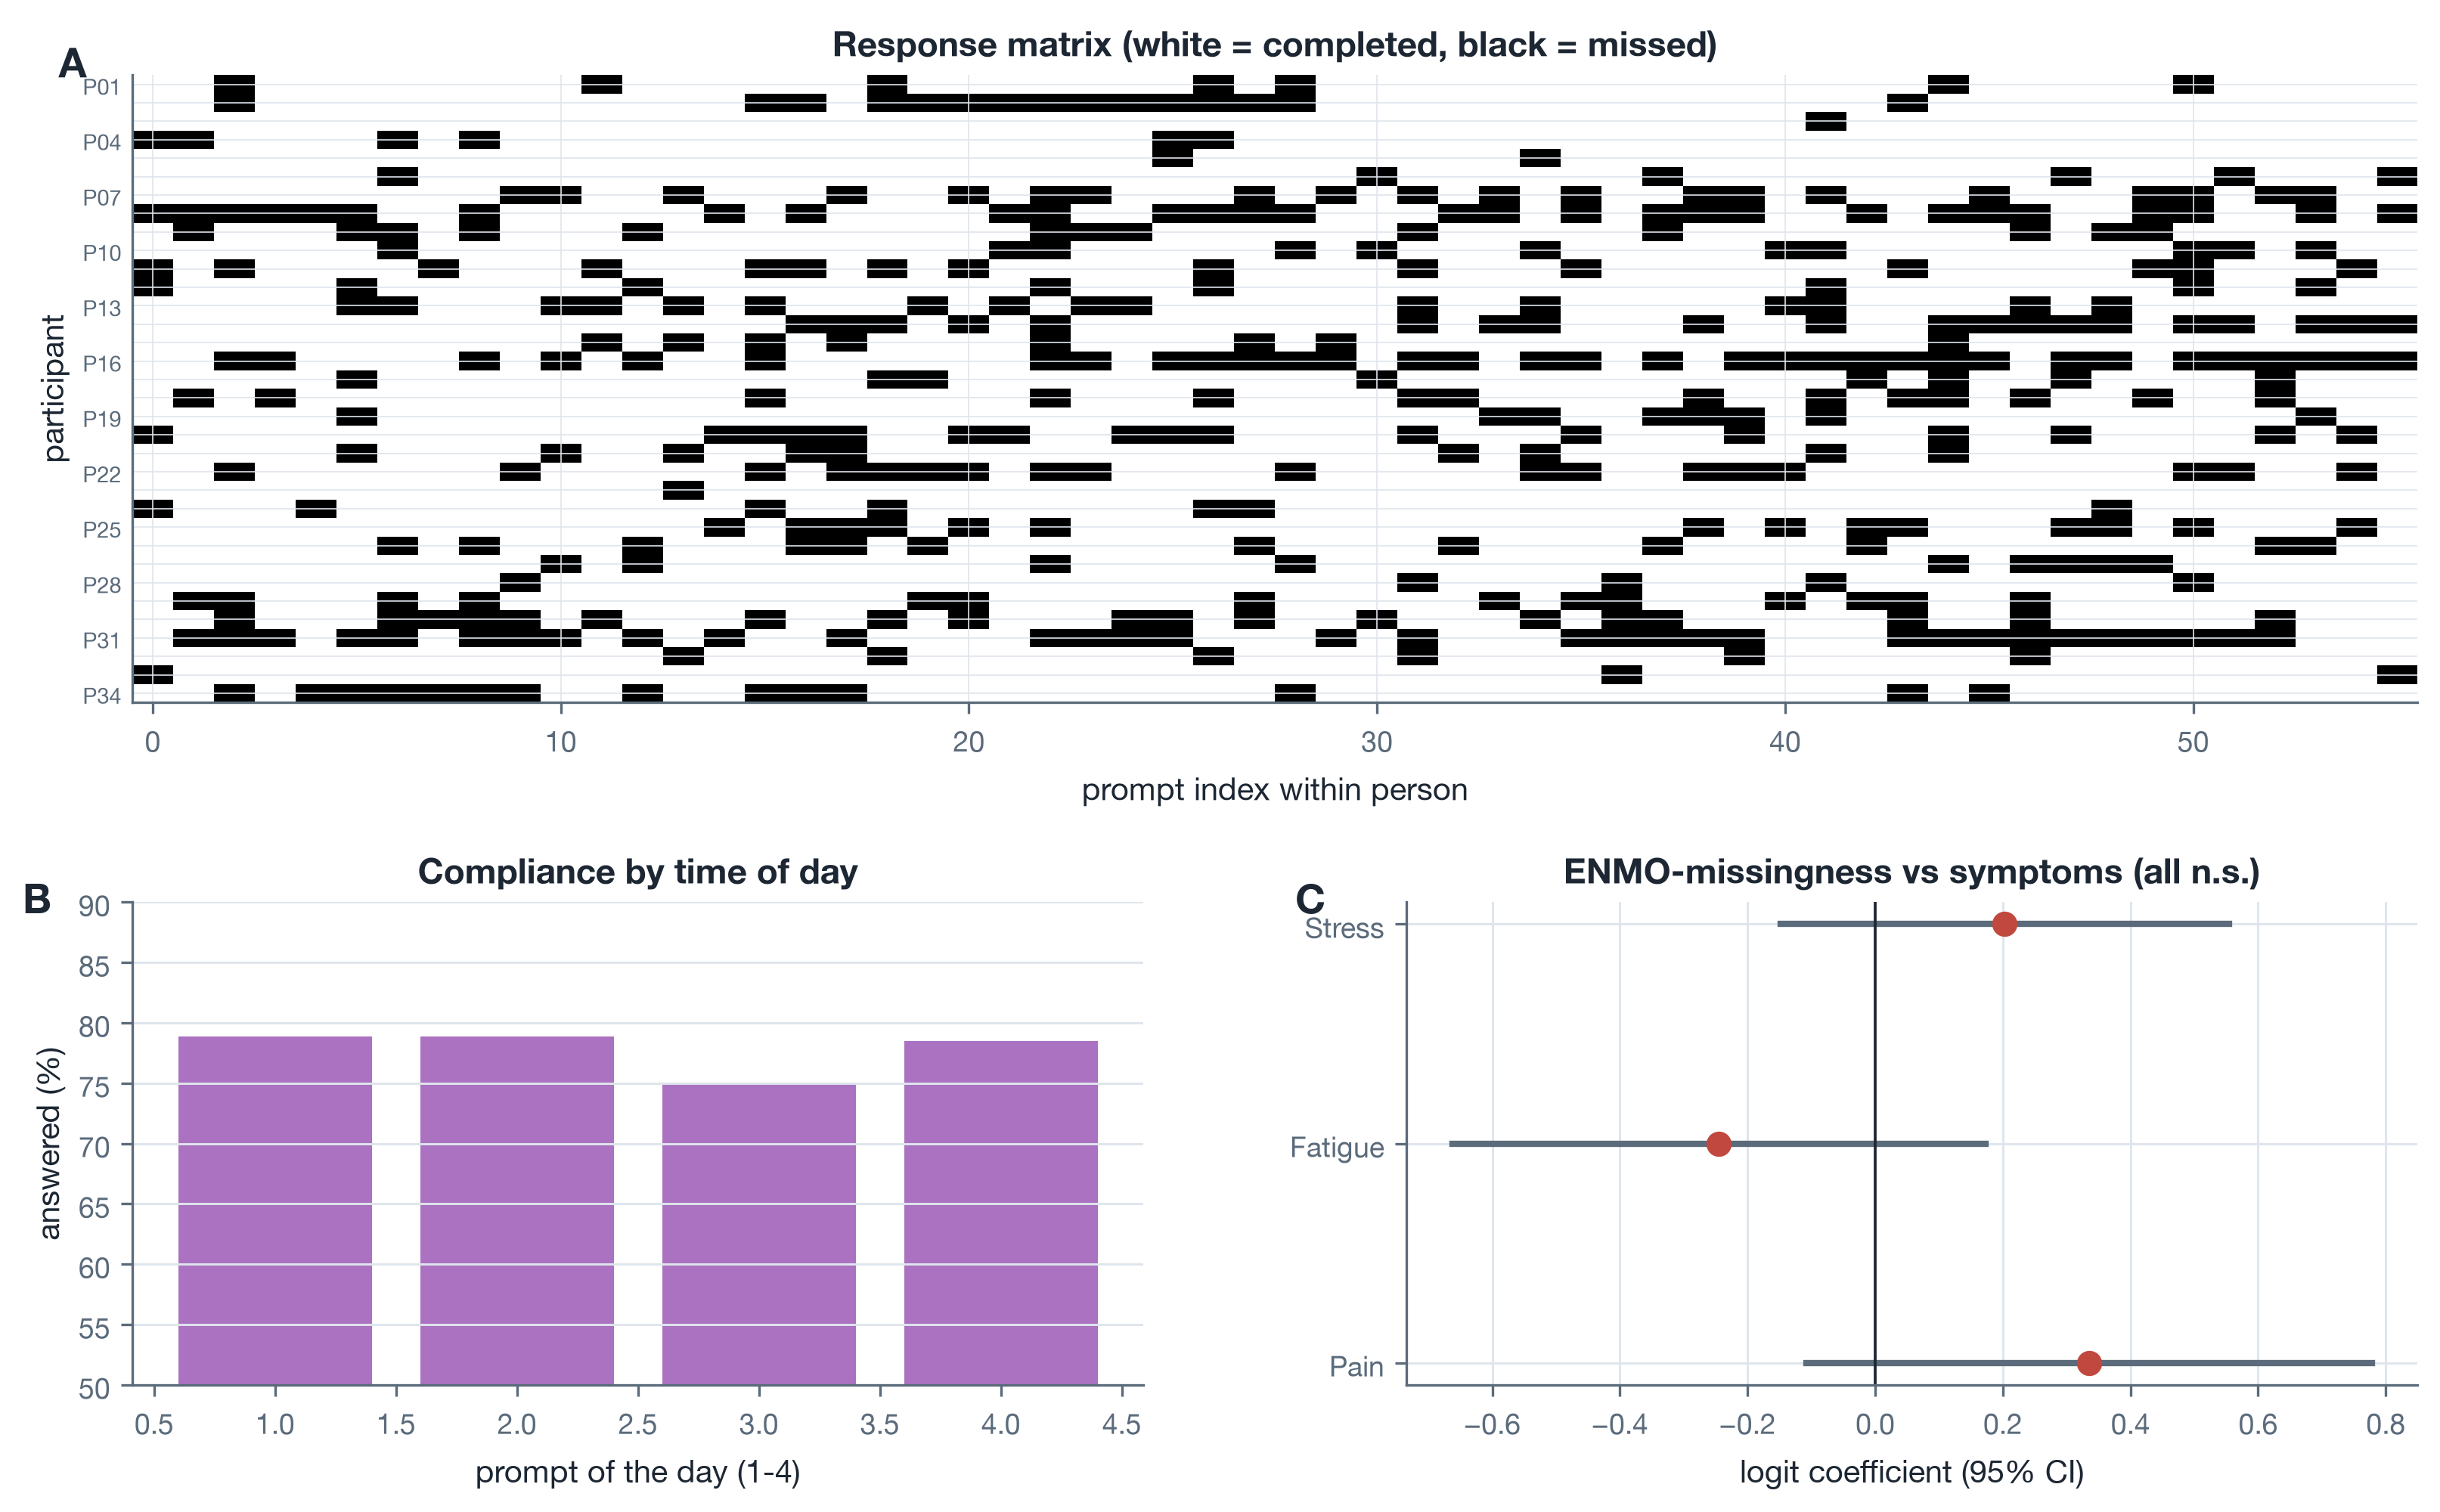
\includegraphics[width=0.92\textwidth]{../assets/figures/supplementary/SUP_04_missingness.png}
\figurenote{Panel A shows the person-by-prompt response matrix (white = completed,
black = missed). Panel B shows compliance by prompt of the day. Panel C shows
logistic-regression probes of objective-activity missingness on momentary pain, fatigue, and
stress, with 95\% confidence intervals.}
\end{figure}

\begin{figure}[H]
\raggedright
\caption{Missing-data imputation benchmark.}
\label{sfig:imputation}
\noindent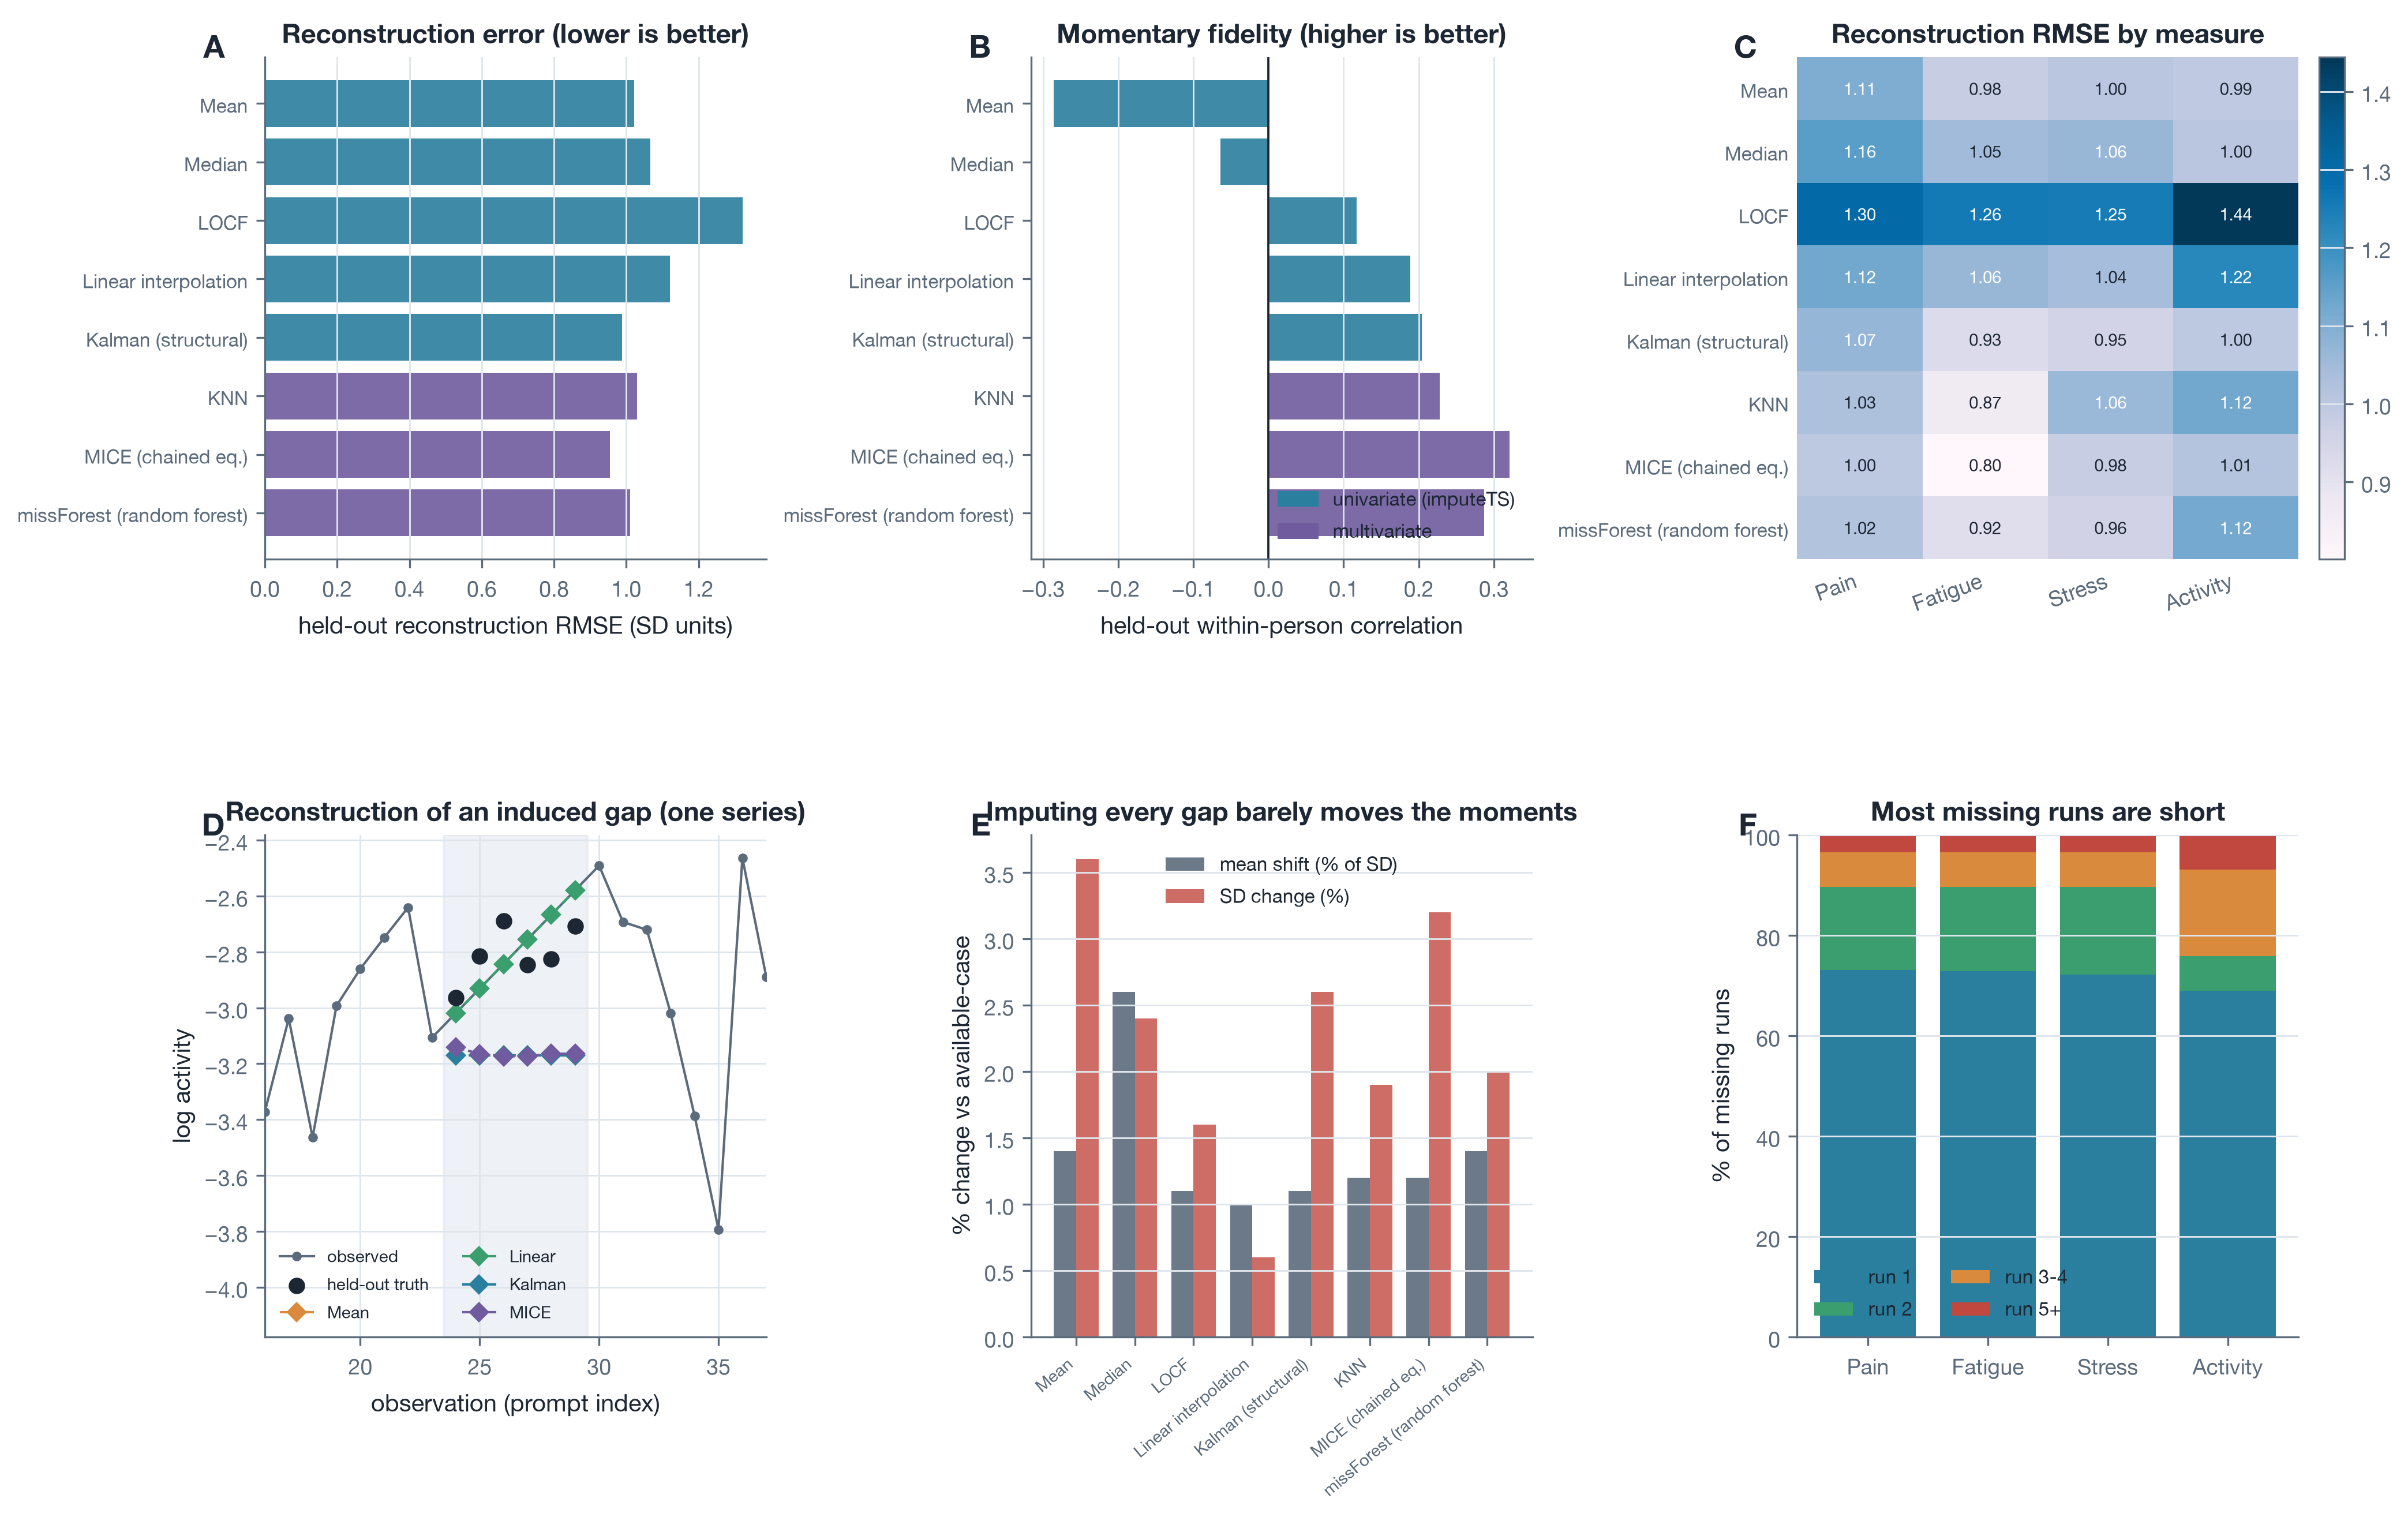
\includegraphics[width=0.92\textwidth]{../assets/figures/supplementary/SUP_05_imputation.png}
\figurenote{Panel A shows the held-out reconstruction error (standardized RMSE) of each
imputation method, and Panel B the within-person held-out correlation; univariate (imputeTS)
methods are shown in teal and multivariate methods in purple. Panel C shows the reconstruction
RMSE of each method by measure. Panel D illustrates each method reconstructing an induced gap
in one within-person activity series. Panel E shows the change in the pooled mean and standard
deviation after every gap is imputed. Panel F shows the distribution of consecutive-missing
run lengths by measure.}
\end{figure}

\begin{figure}[H]
\raggedright
\caption{Feasibility of fully idiographic networks.}
\label{sfig:feasibility}
\noindent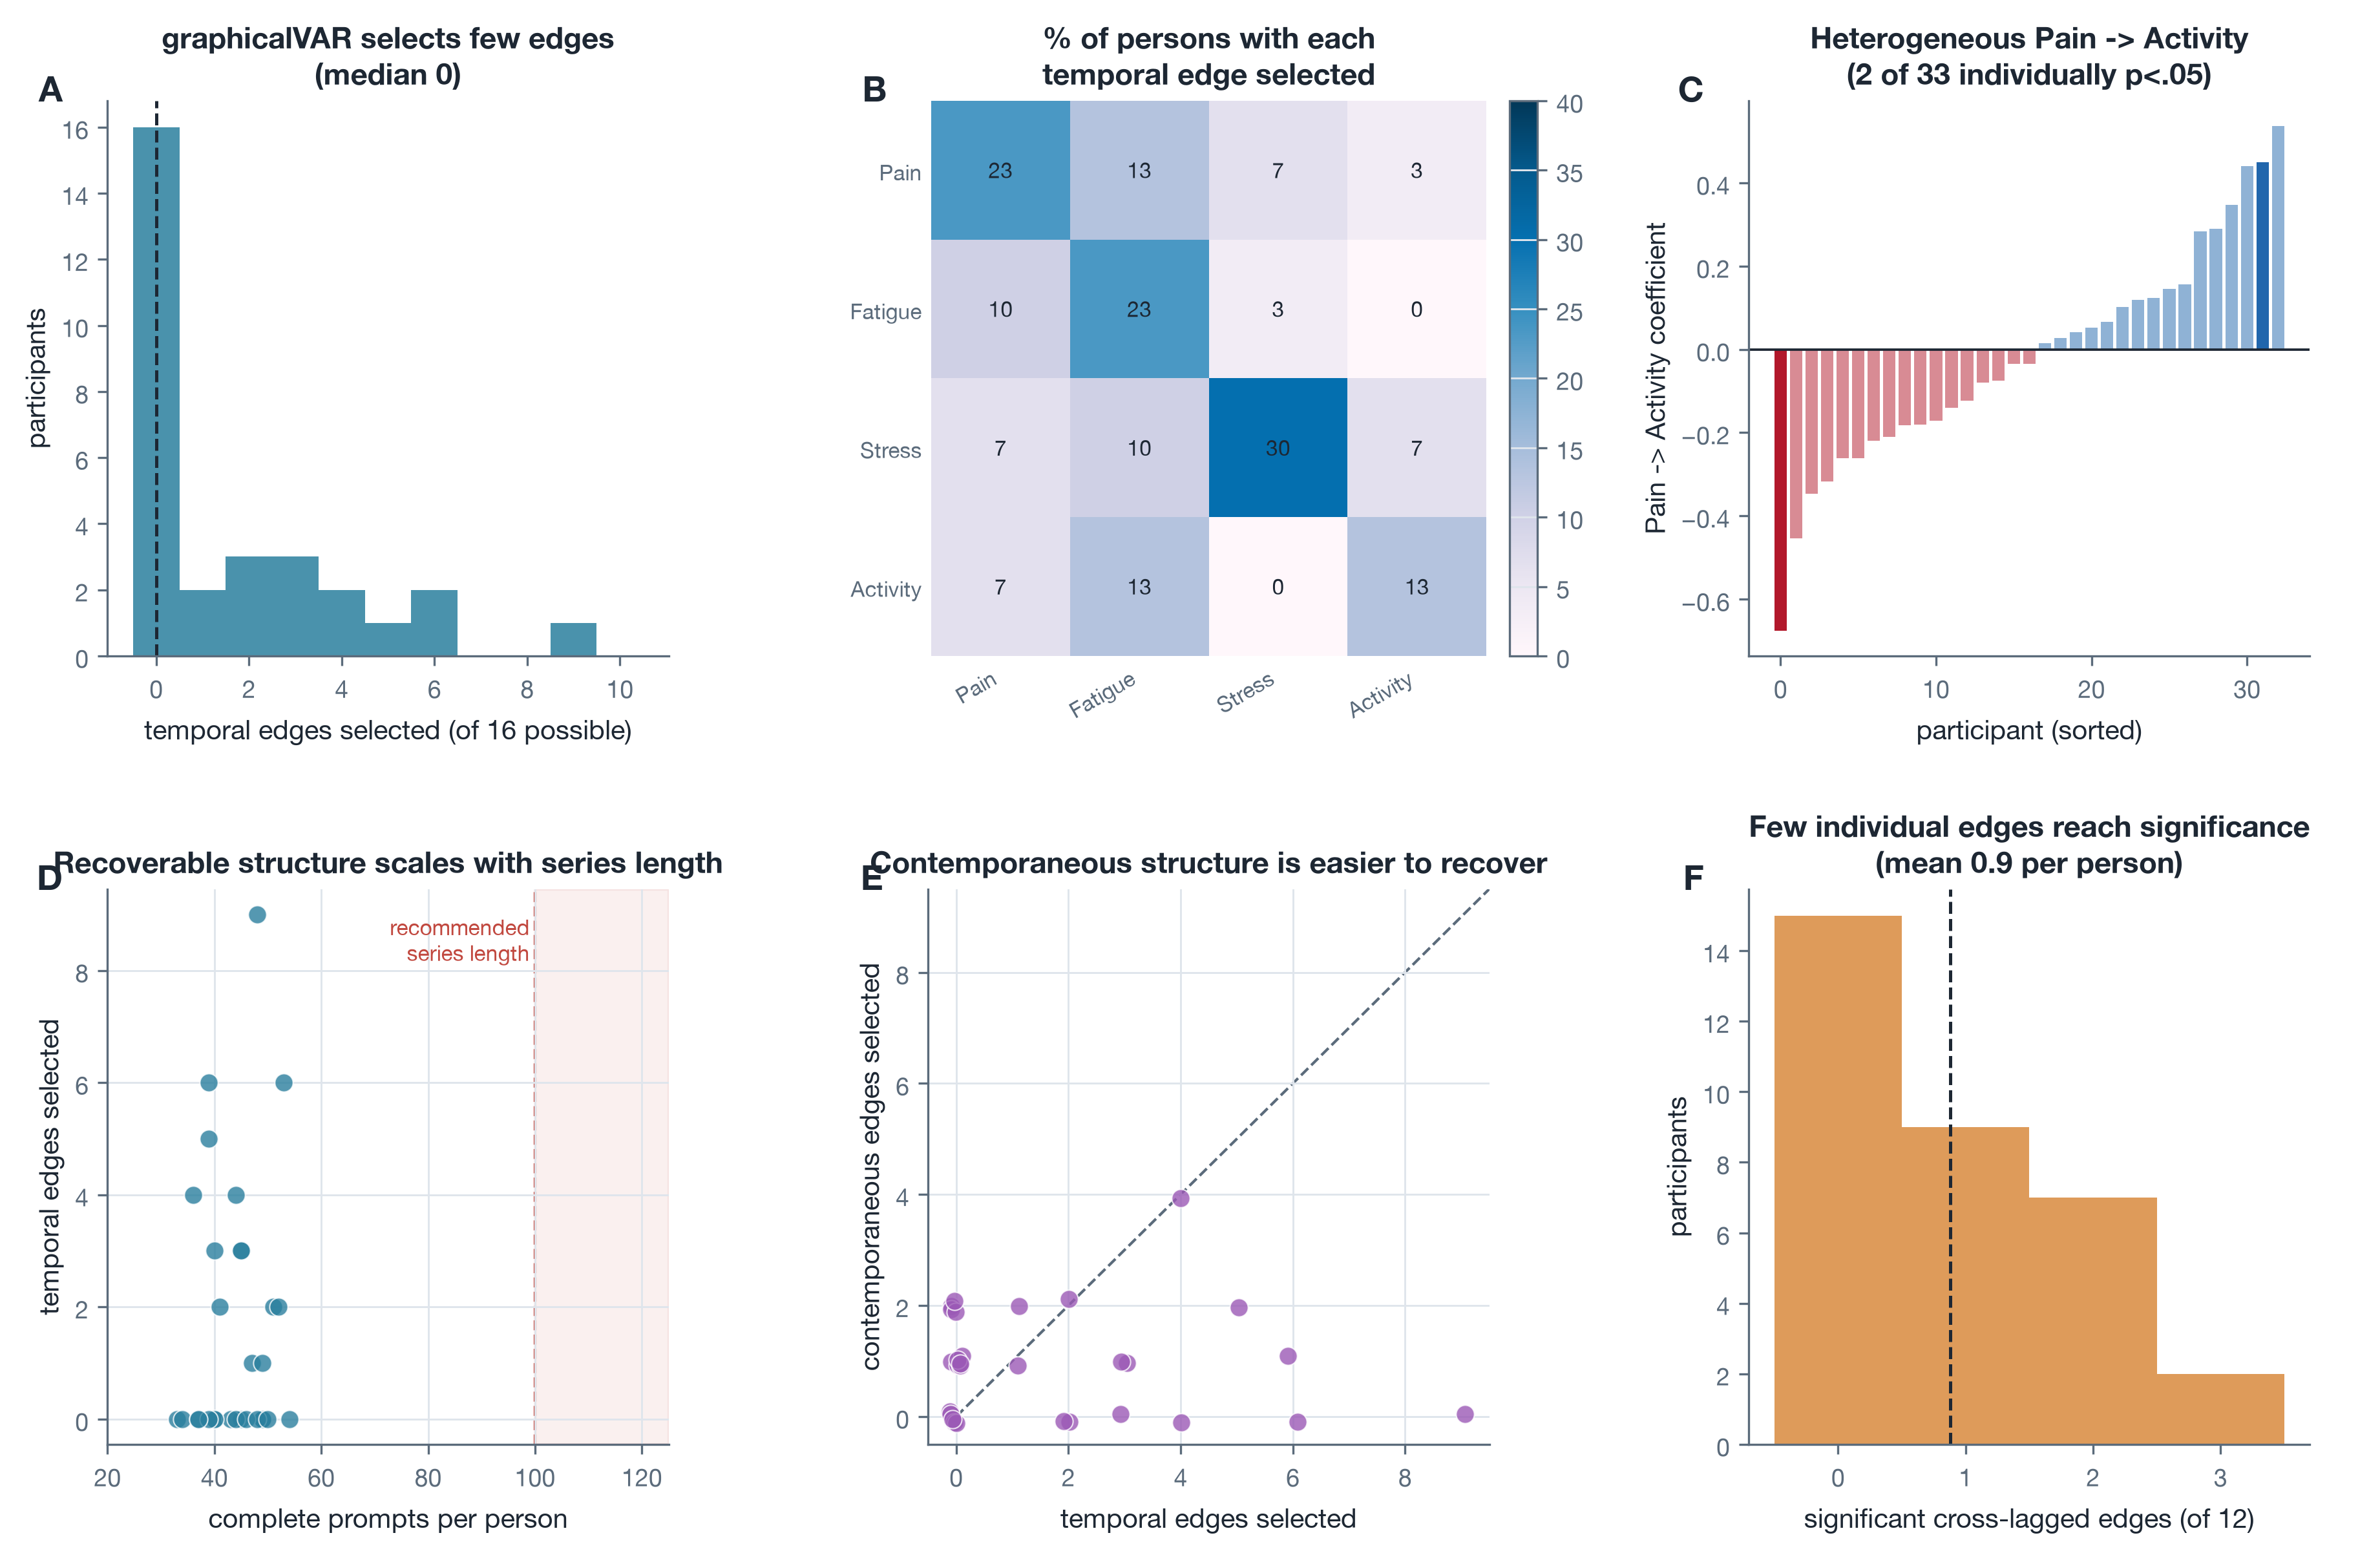
\includegraphics[width=0.92\textwidth]{../assets/figures/supplementary/SUP_06_idiographic_feasibility.png}
\figurenote{Panel A shows the number of graphicalVAR temporal edges selected per person.
Panel B shows the percentage of persons for whom each directed temporal edge was selected.
Panel C shows the sorted per-person unregularized pain-to-activity coefficients, with
individually significant values highlighted. Panel D plots the number of temporal edges
selected against the number of complete prompts, with the recommended series length marked.
Panel E compares the number of contemporaneous and temporal edges selected per person.
Panel F shows the number of individually significant unregularized cross-lagged edges per
person.}
\end{figure}

\begin{figure}[H]
\raggedright
\caption{S-GIMME subgroup structure and path prevalence.}
\label{sfig:sgimme}
\noindent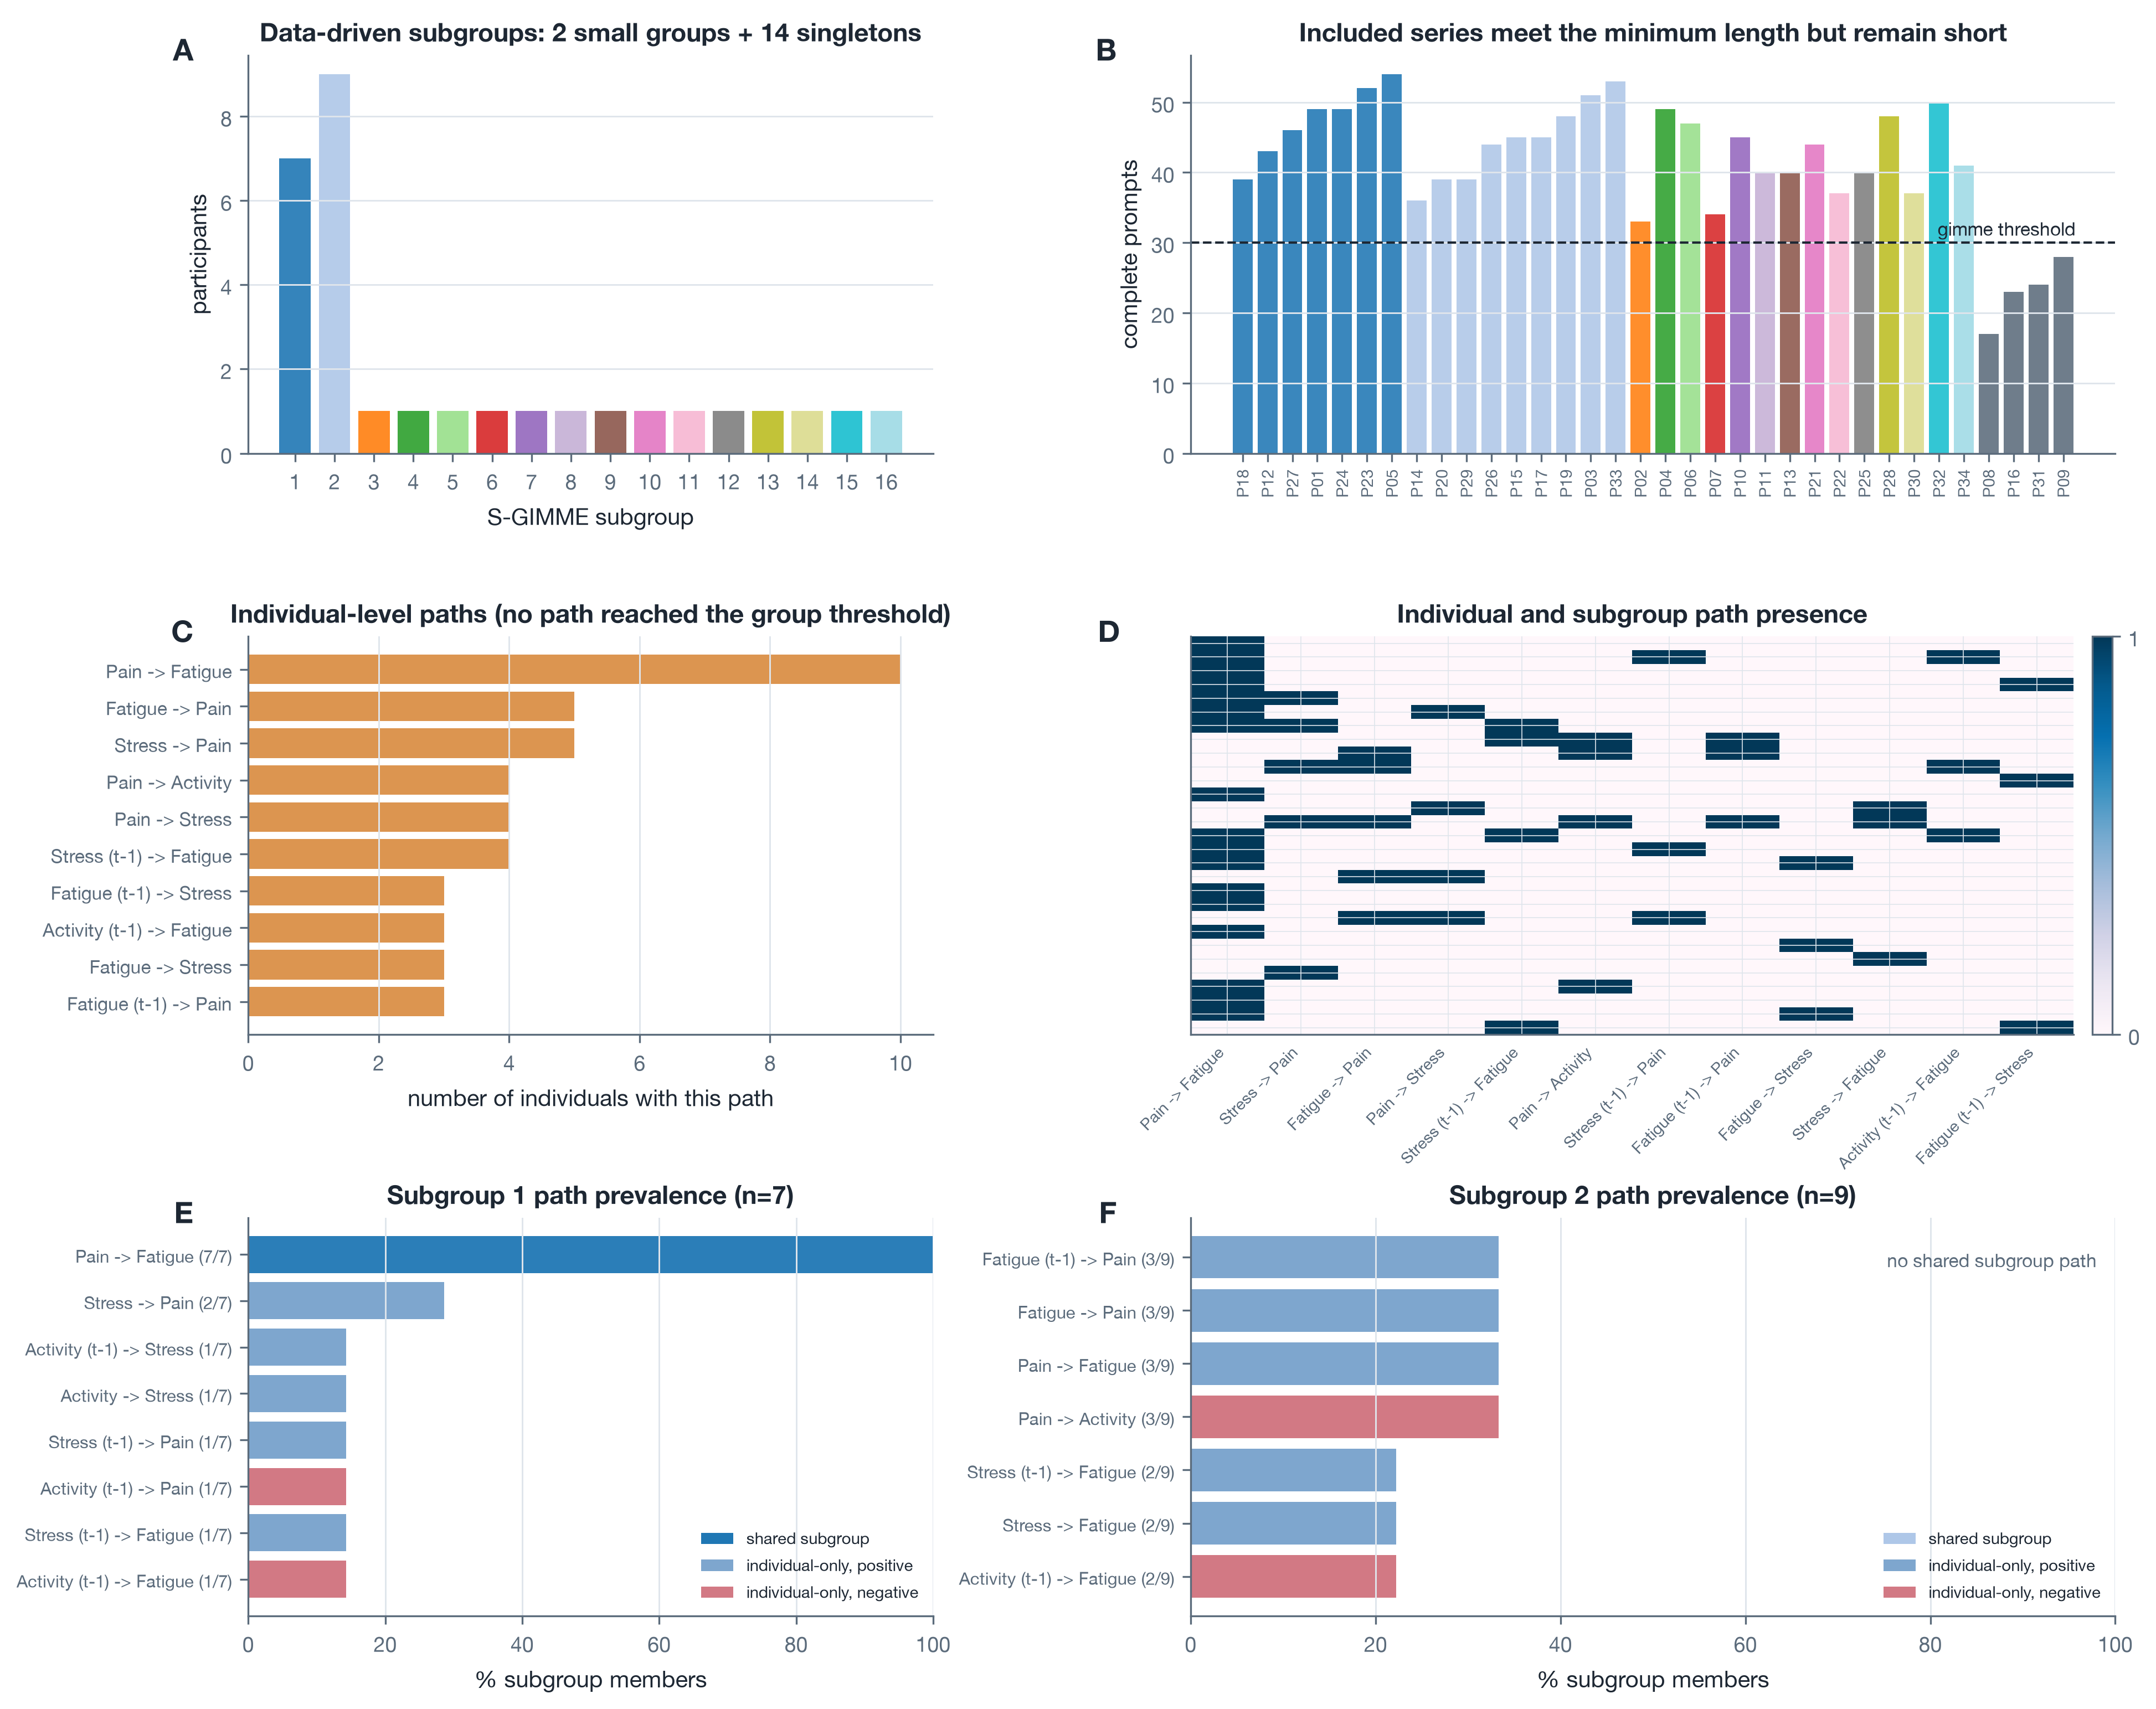
\includegraphics[width=0.96\textwidth]{../assets/figures/supplementary/SUP_07_sgimme.png}
\figurenote{Panel A shows the S-GIMME subgroup sizes. Panel B shows the number of complete
prompts per participant relative to the gimme minimum, coloured by subgroup. Panel C shows
the most frequent individual-level paths. Panel D shows individual and subgroup path presence,
ordered by S-GIMME subgroup. Panels E and F show path prevalence within the two multi-person
S-GIMME subgroups, distinguishing shared subgroup-level paths from individual-only paths.}
\end{figure}

\begin{figure}[H]
\raggedright
\caption{Extended six-node and seven-node mlVAR models.}
\label{sfig:extended}
\noindent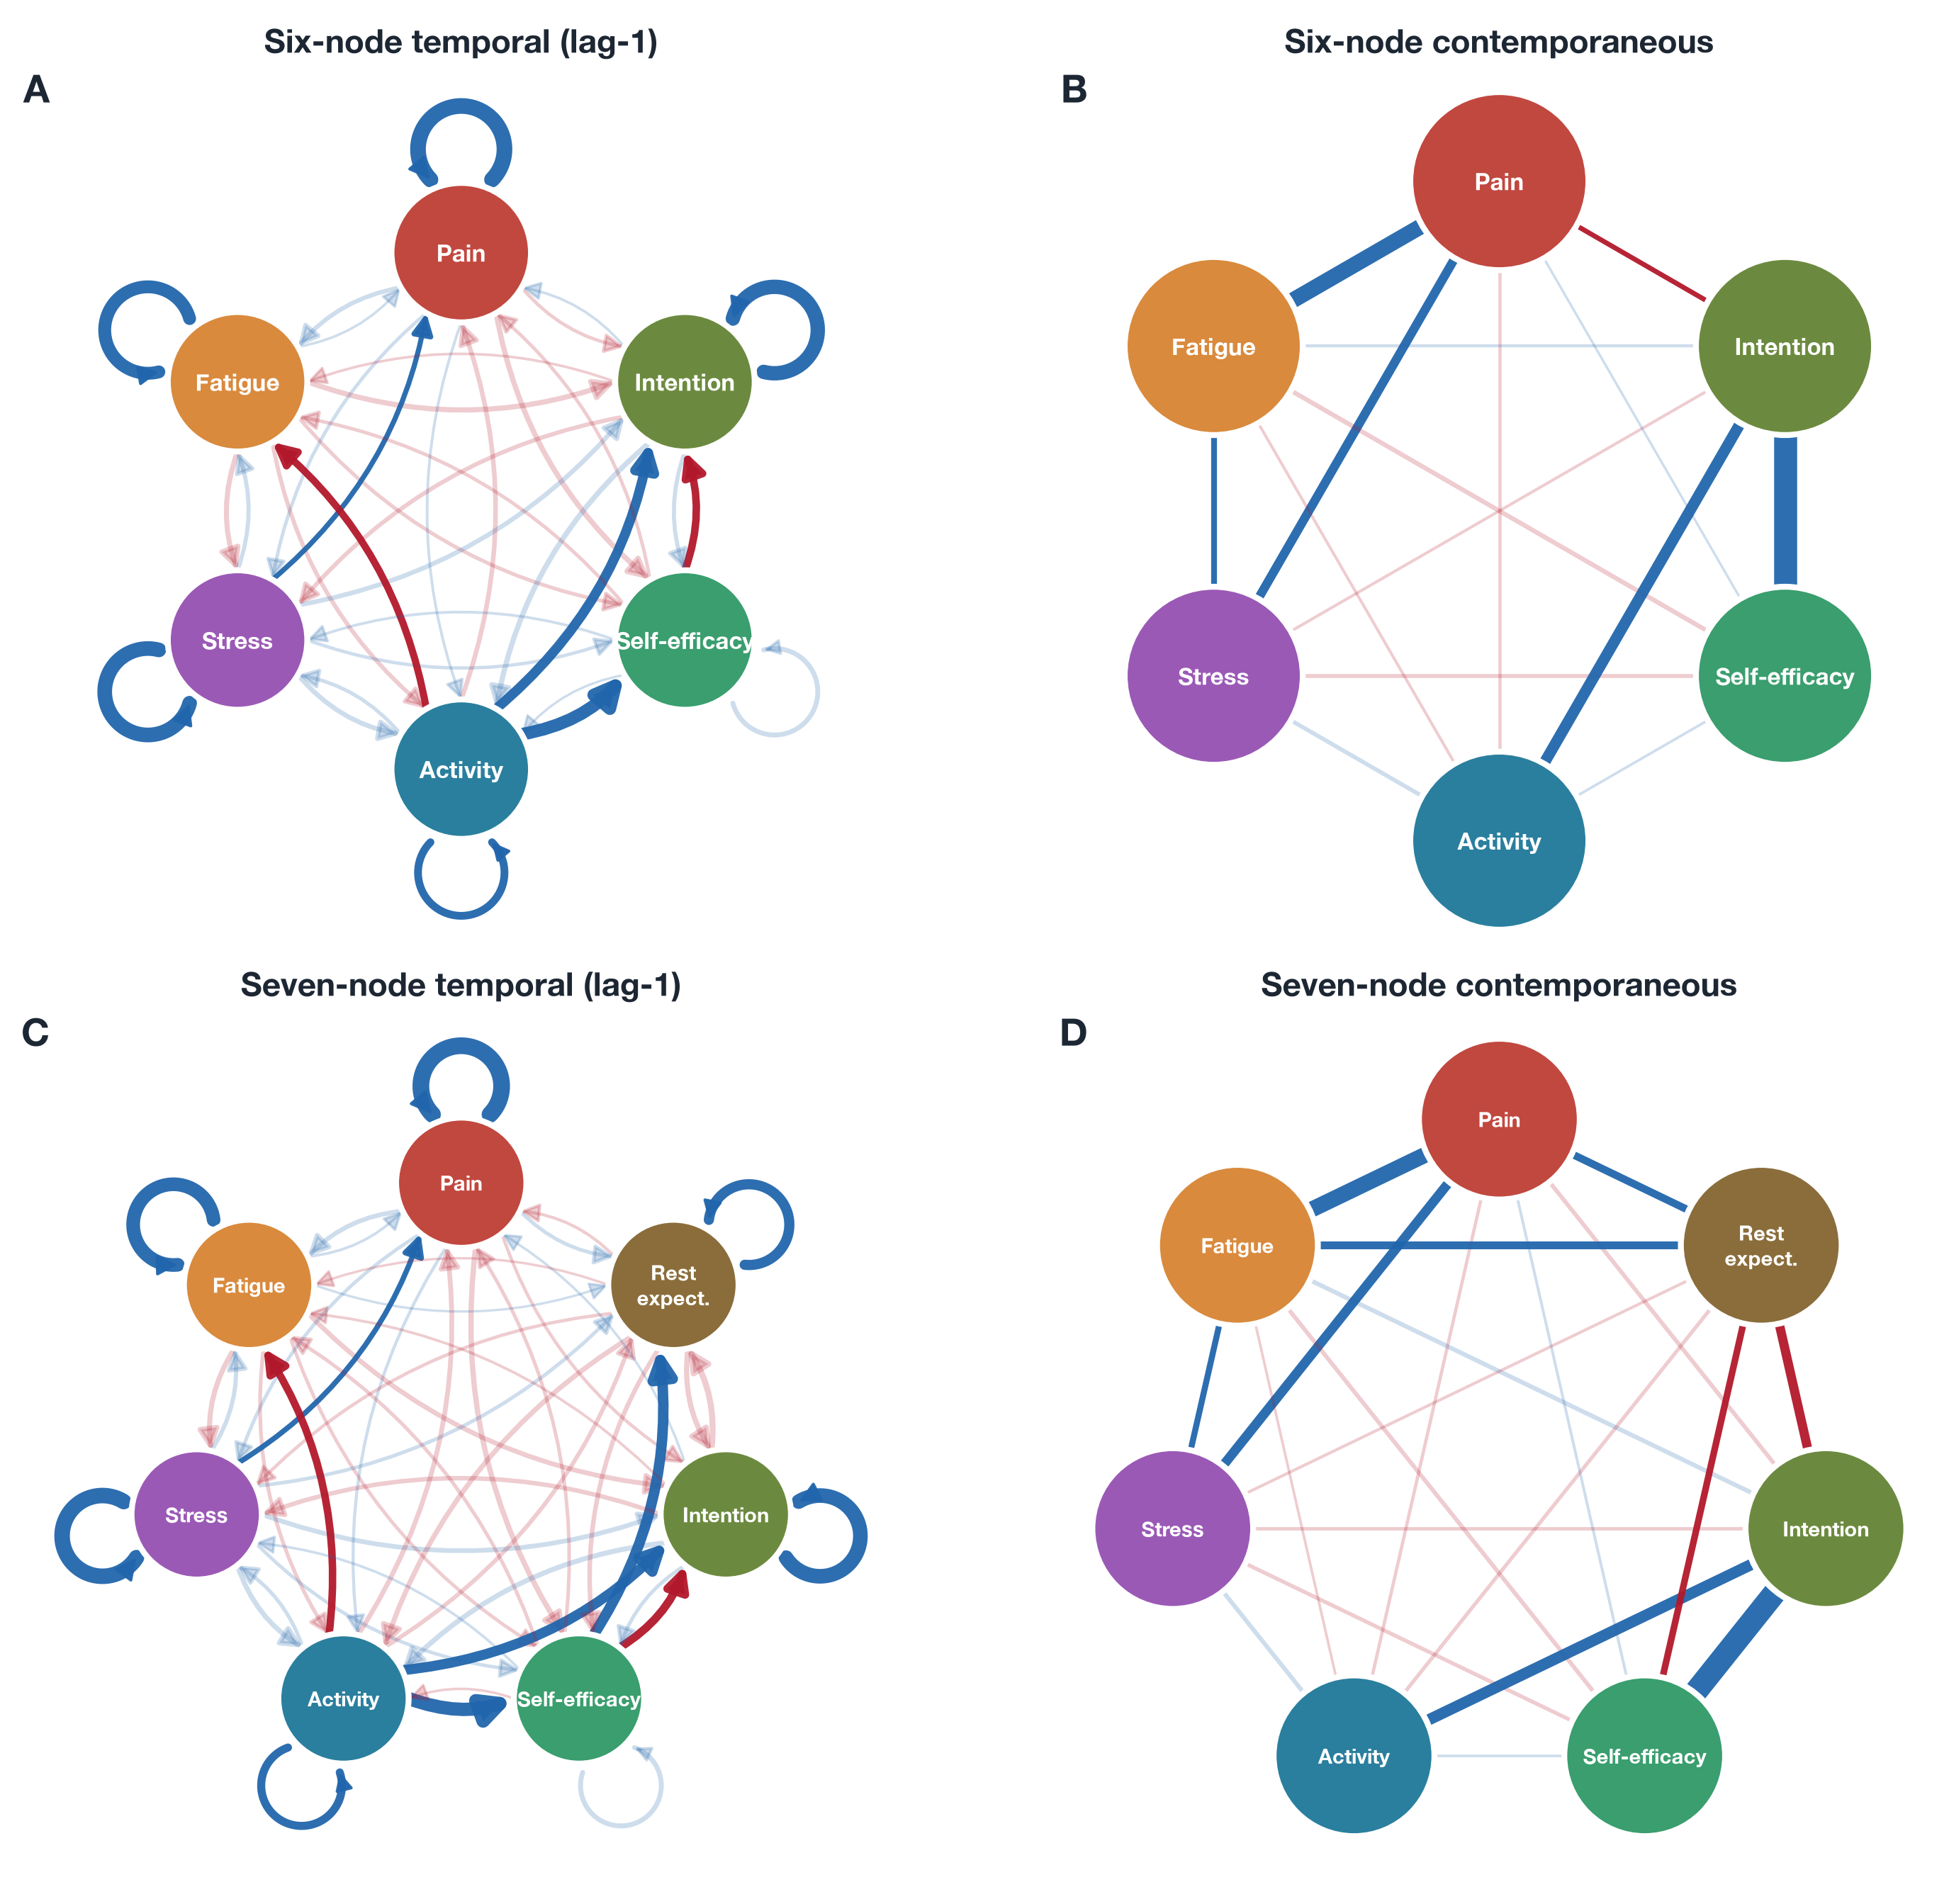
\includegraphics[width=0.96\textwidth]{../assets/figures/supplementary/SUP_08_extended_network.png}
\figurenote{Panels A and B show the temporal and contemporaneous networks of the extended
six-node model, which adds momentary self-efficacy and intention to the four core nodes.
Panels C and D show the corresponding seven-node model, which additionally adds
rest-favouring outcome expectancy. Blue edges are positive, red edges are negative, and edge
width scales with strength.}
\end{figure}

\begin{figure}[H]
\raggedright
\caption{Could-not-move sensitivity analysis.}
\label{sfig:cantmove}
\noindent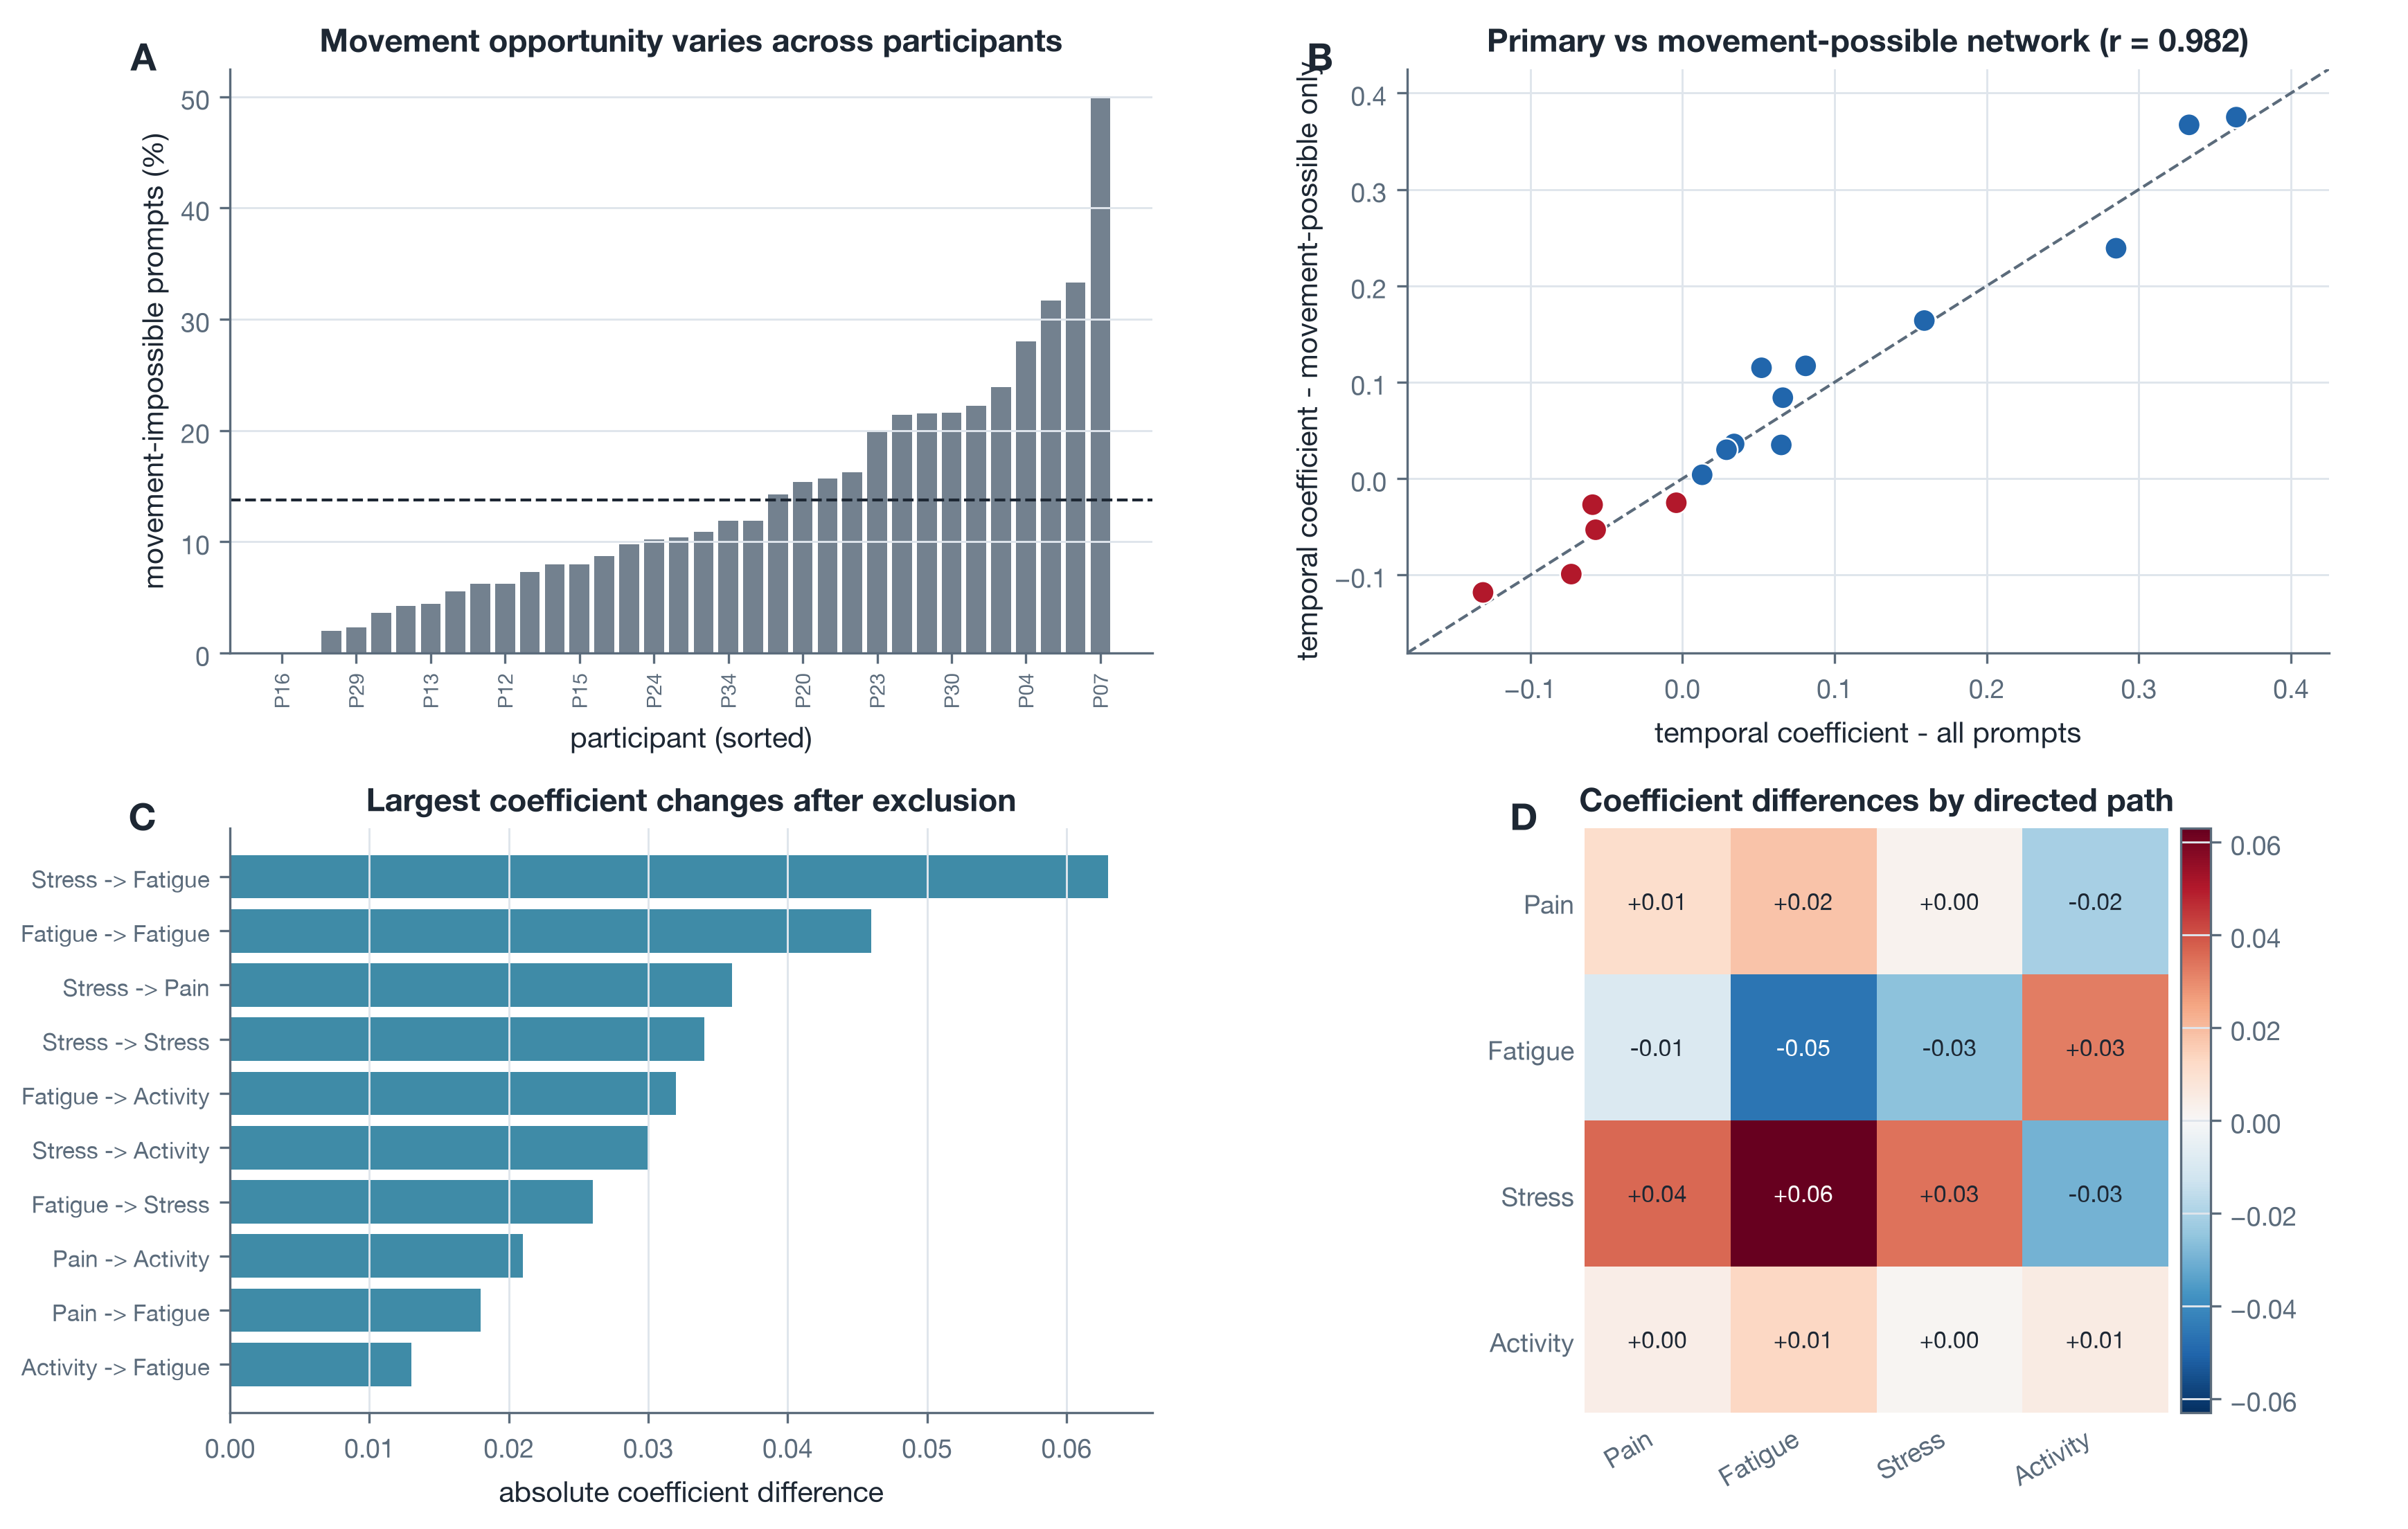
\includegraphics[width=0.92\textwidth]{../assets/figures/supplementary/SUP_09_cantmove_sensitivity.png}
\figurenote{Panel A shows the participant-level percentage of prompts where movement was
reported as impossible. Panel B compares primary temporal coefficients with coefficients
from the model restricted to movement-possible prompts. Panel C ranks the largest absolute
coefficient changes. Panel D maps coefficient differences for each directed temporal path.}
\end{figure}

\begin{figure}[H]
\raggedright
\caption{Momentary pacing behaviours.}
\label{sfig:pacing}
\noindent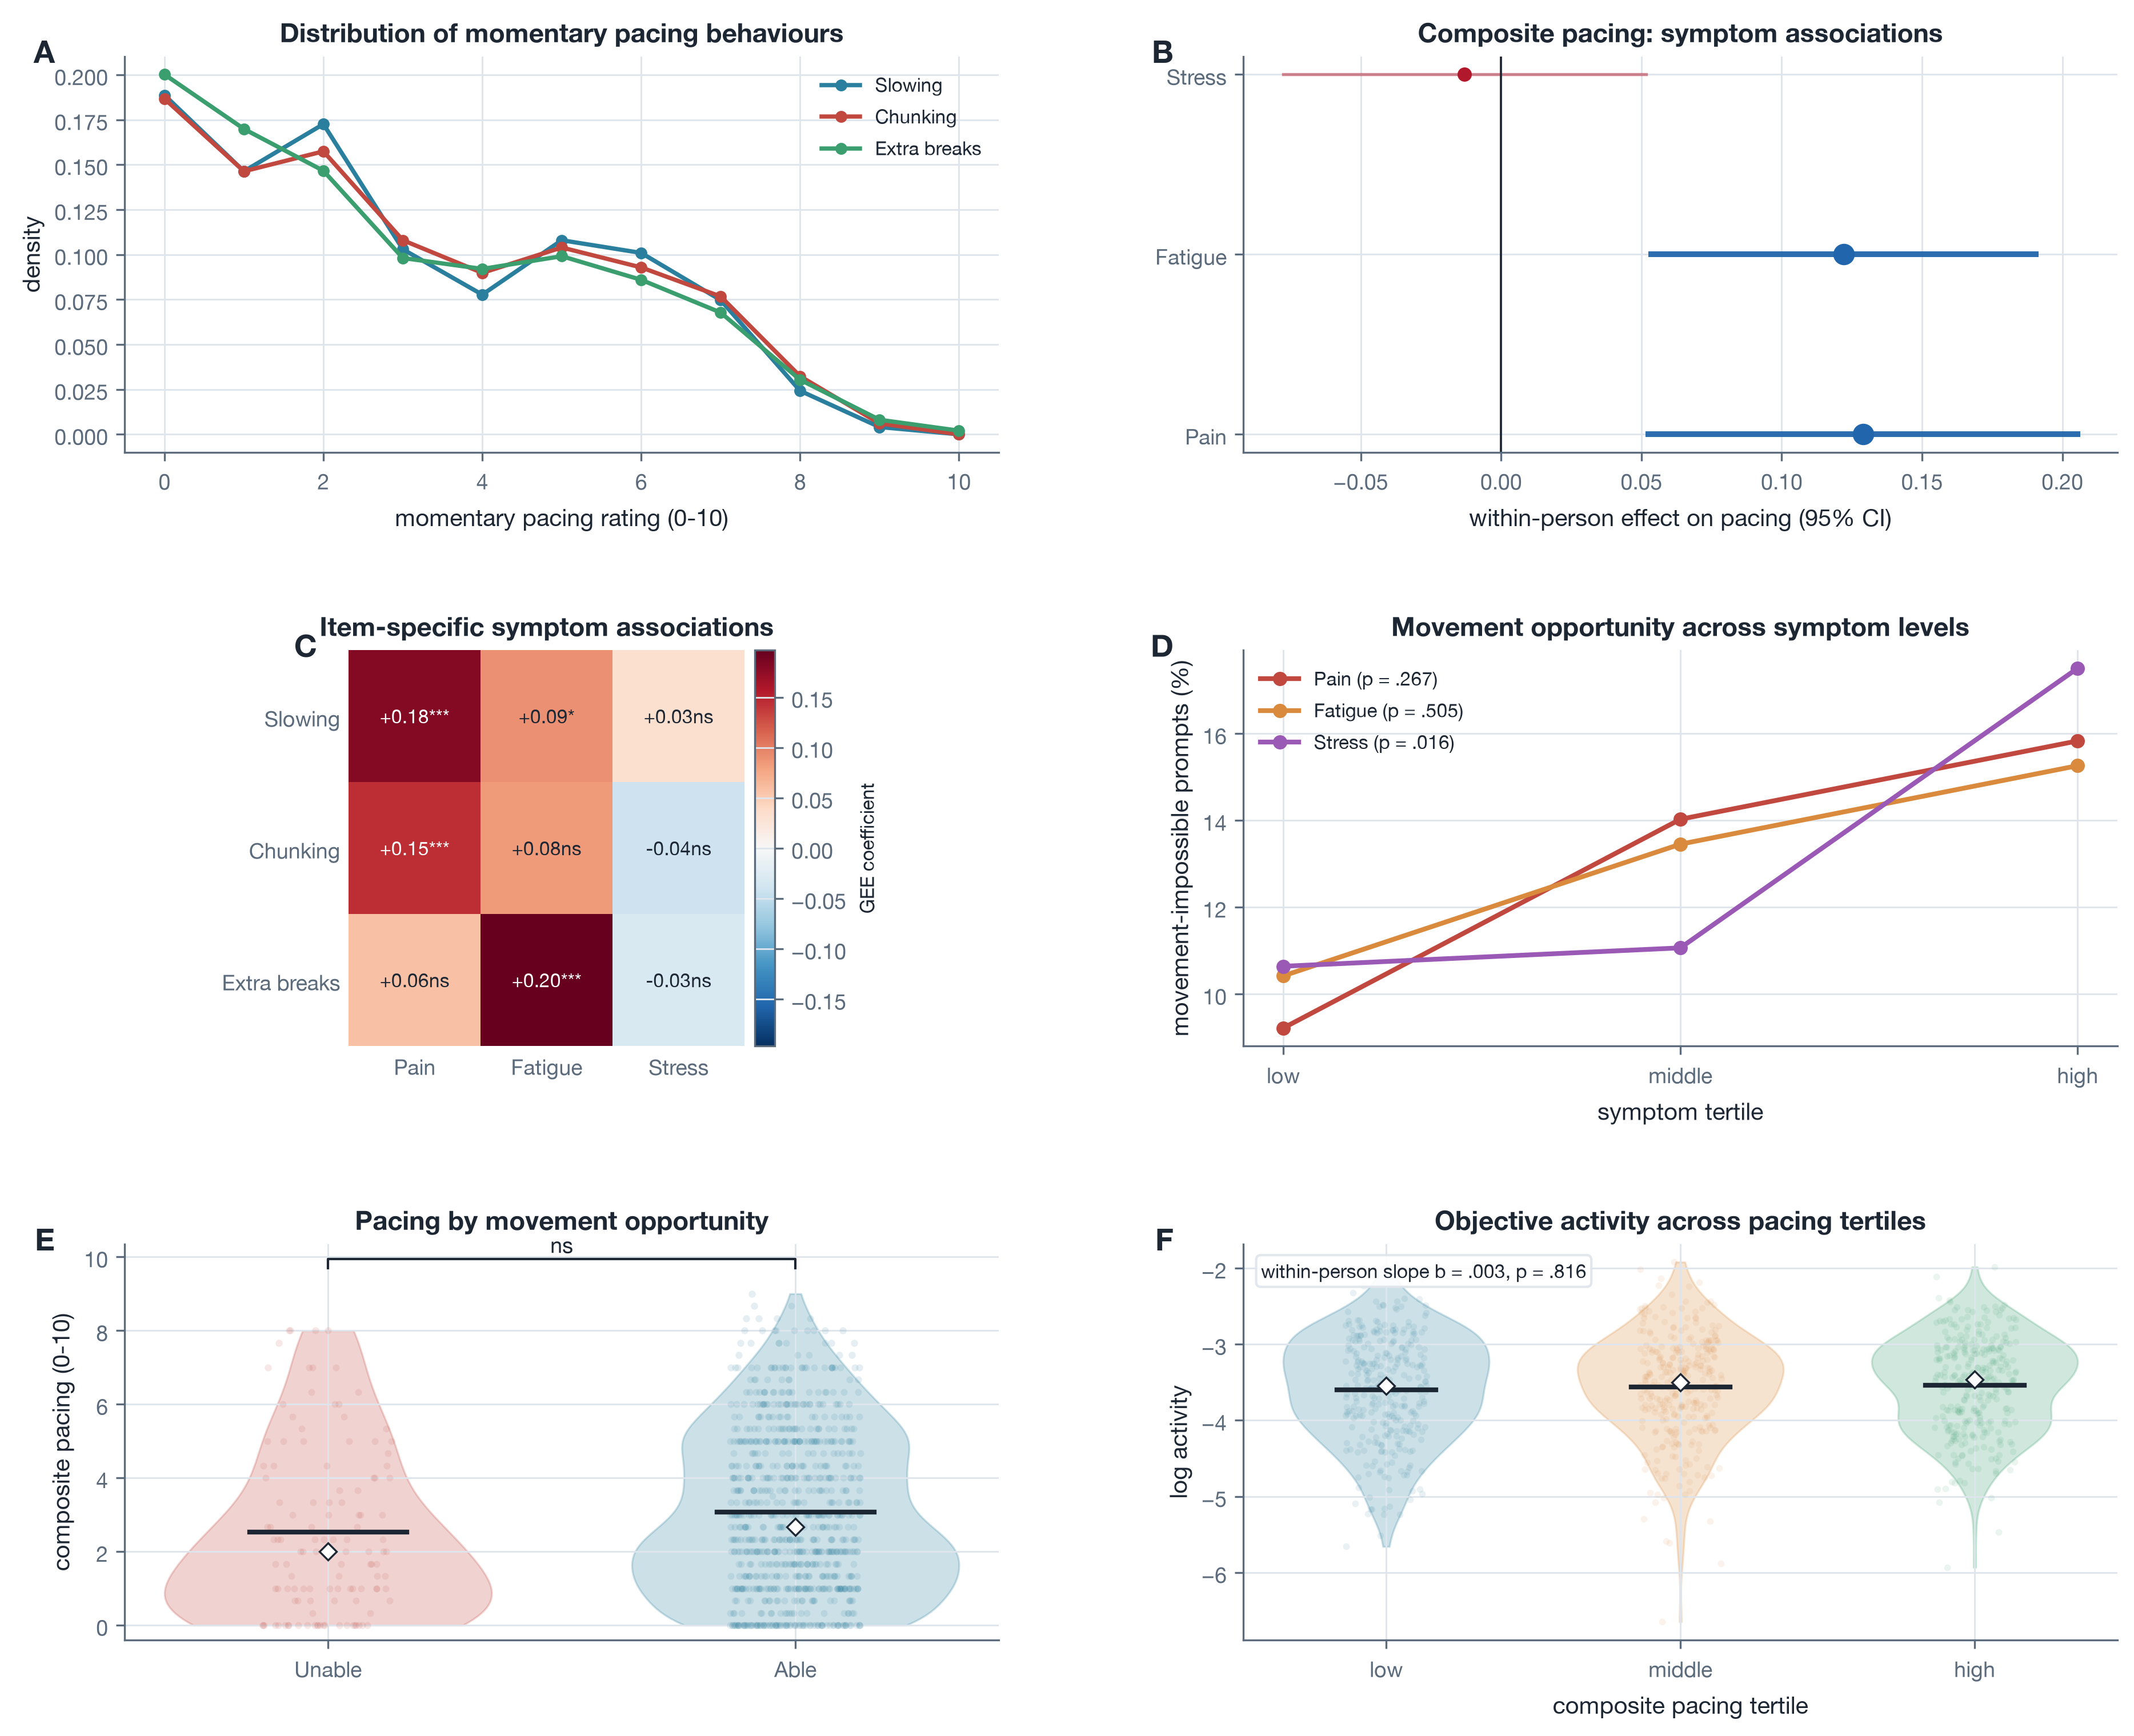
\includegraphics[width=0.96\textwidth]{../assets/figures/supplementary/SUP_10_pacing.png}
\figurenote{Panel A shows the distributions of the three momentary pacing items (deliberate
slowing, breaking tasks into parts, and inserting extra breaks). Panel B shows within-person
associations of momentary pain, fatigue, and stress with the composite pacing score, with
95\% confidence intervals. Panel C shows item-specific within-person symptom effects from
participant-clustered Gaussian GEE models. Panel D shows the percentage of prompts at which
movement was impossible across symptom tertiles. Panel E compares composite pacing when
participants were able versus unable to move, using raw prompt-level distributions, means,
medians, and a Gaussian GEE significance bar. Panel F compares objective activity across
composite-pacing tertiles and gives the within-person pacing-to-activity slope.}
\end{figure}

\begin{figure}[H]
\raggedright
\caption{Within-person and between-person correlations.}
\label{sfig:correlations}
\noindent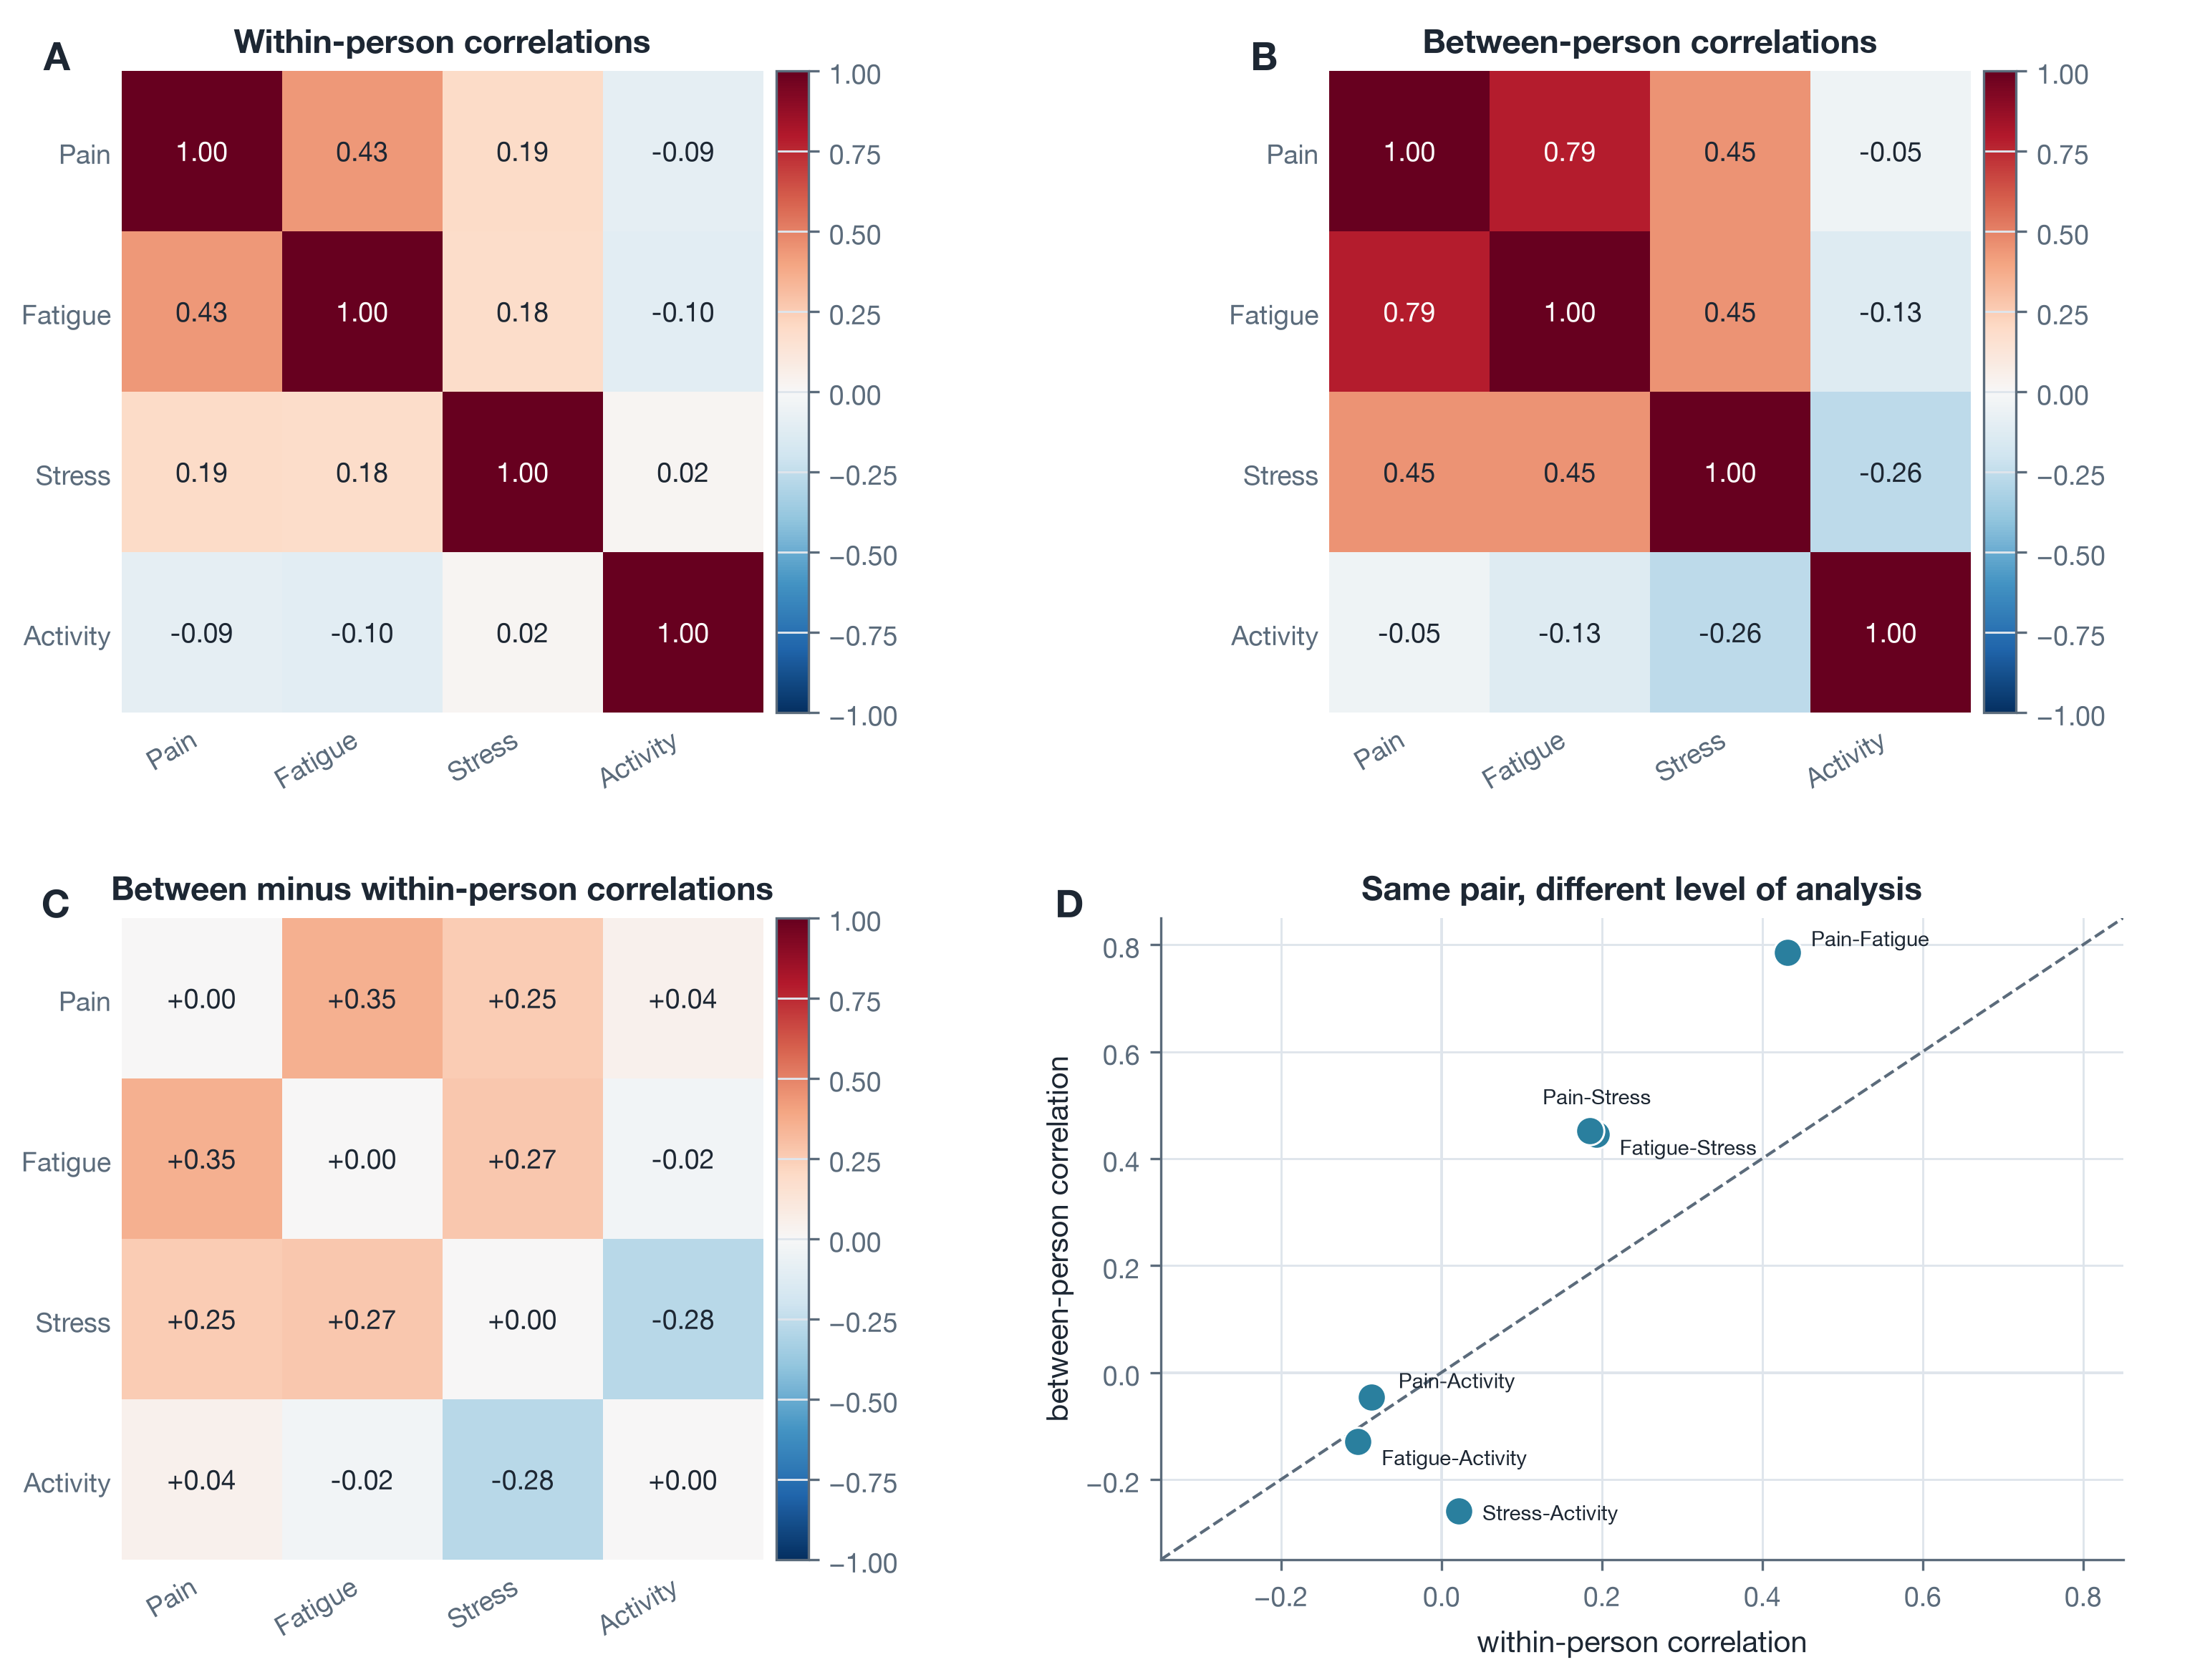
\includegraphics[width=0.92\textwidth]{../assets/figures/supplementary/SUP_11_within_between_correlations.png}
\figurenote{Panel A shows correlations after within-person centring. Panel B shows
correlations among person means. Panel C displays the between-person minus within-person
difference matrix. Panel D plots each pair at both levels to show where association patterns
change across levels of analysis.}
\end{figure}

\begin{figure}[H]
\raggedright
\caption{Robustness of the temporal network.}
\label{sfig:robustness}
\noindent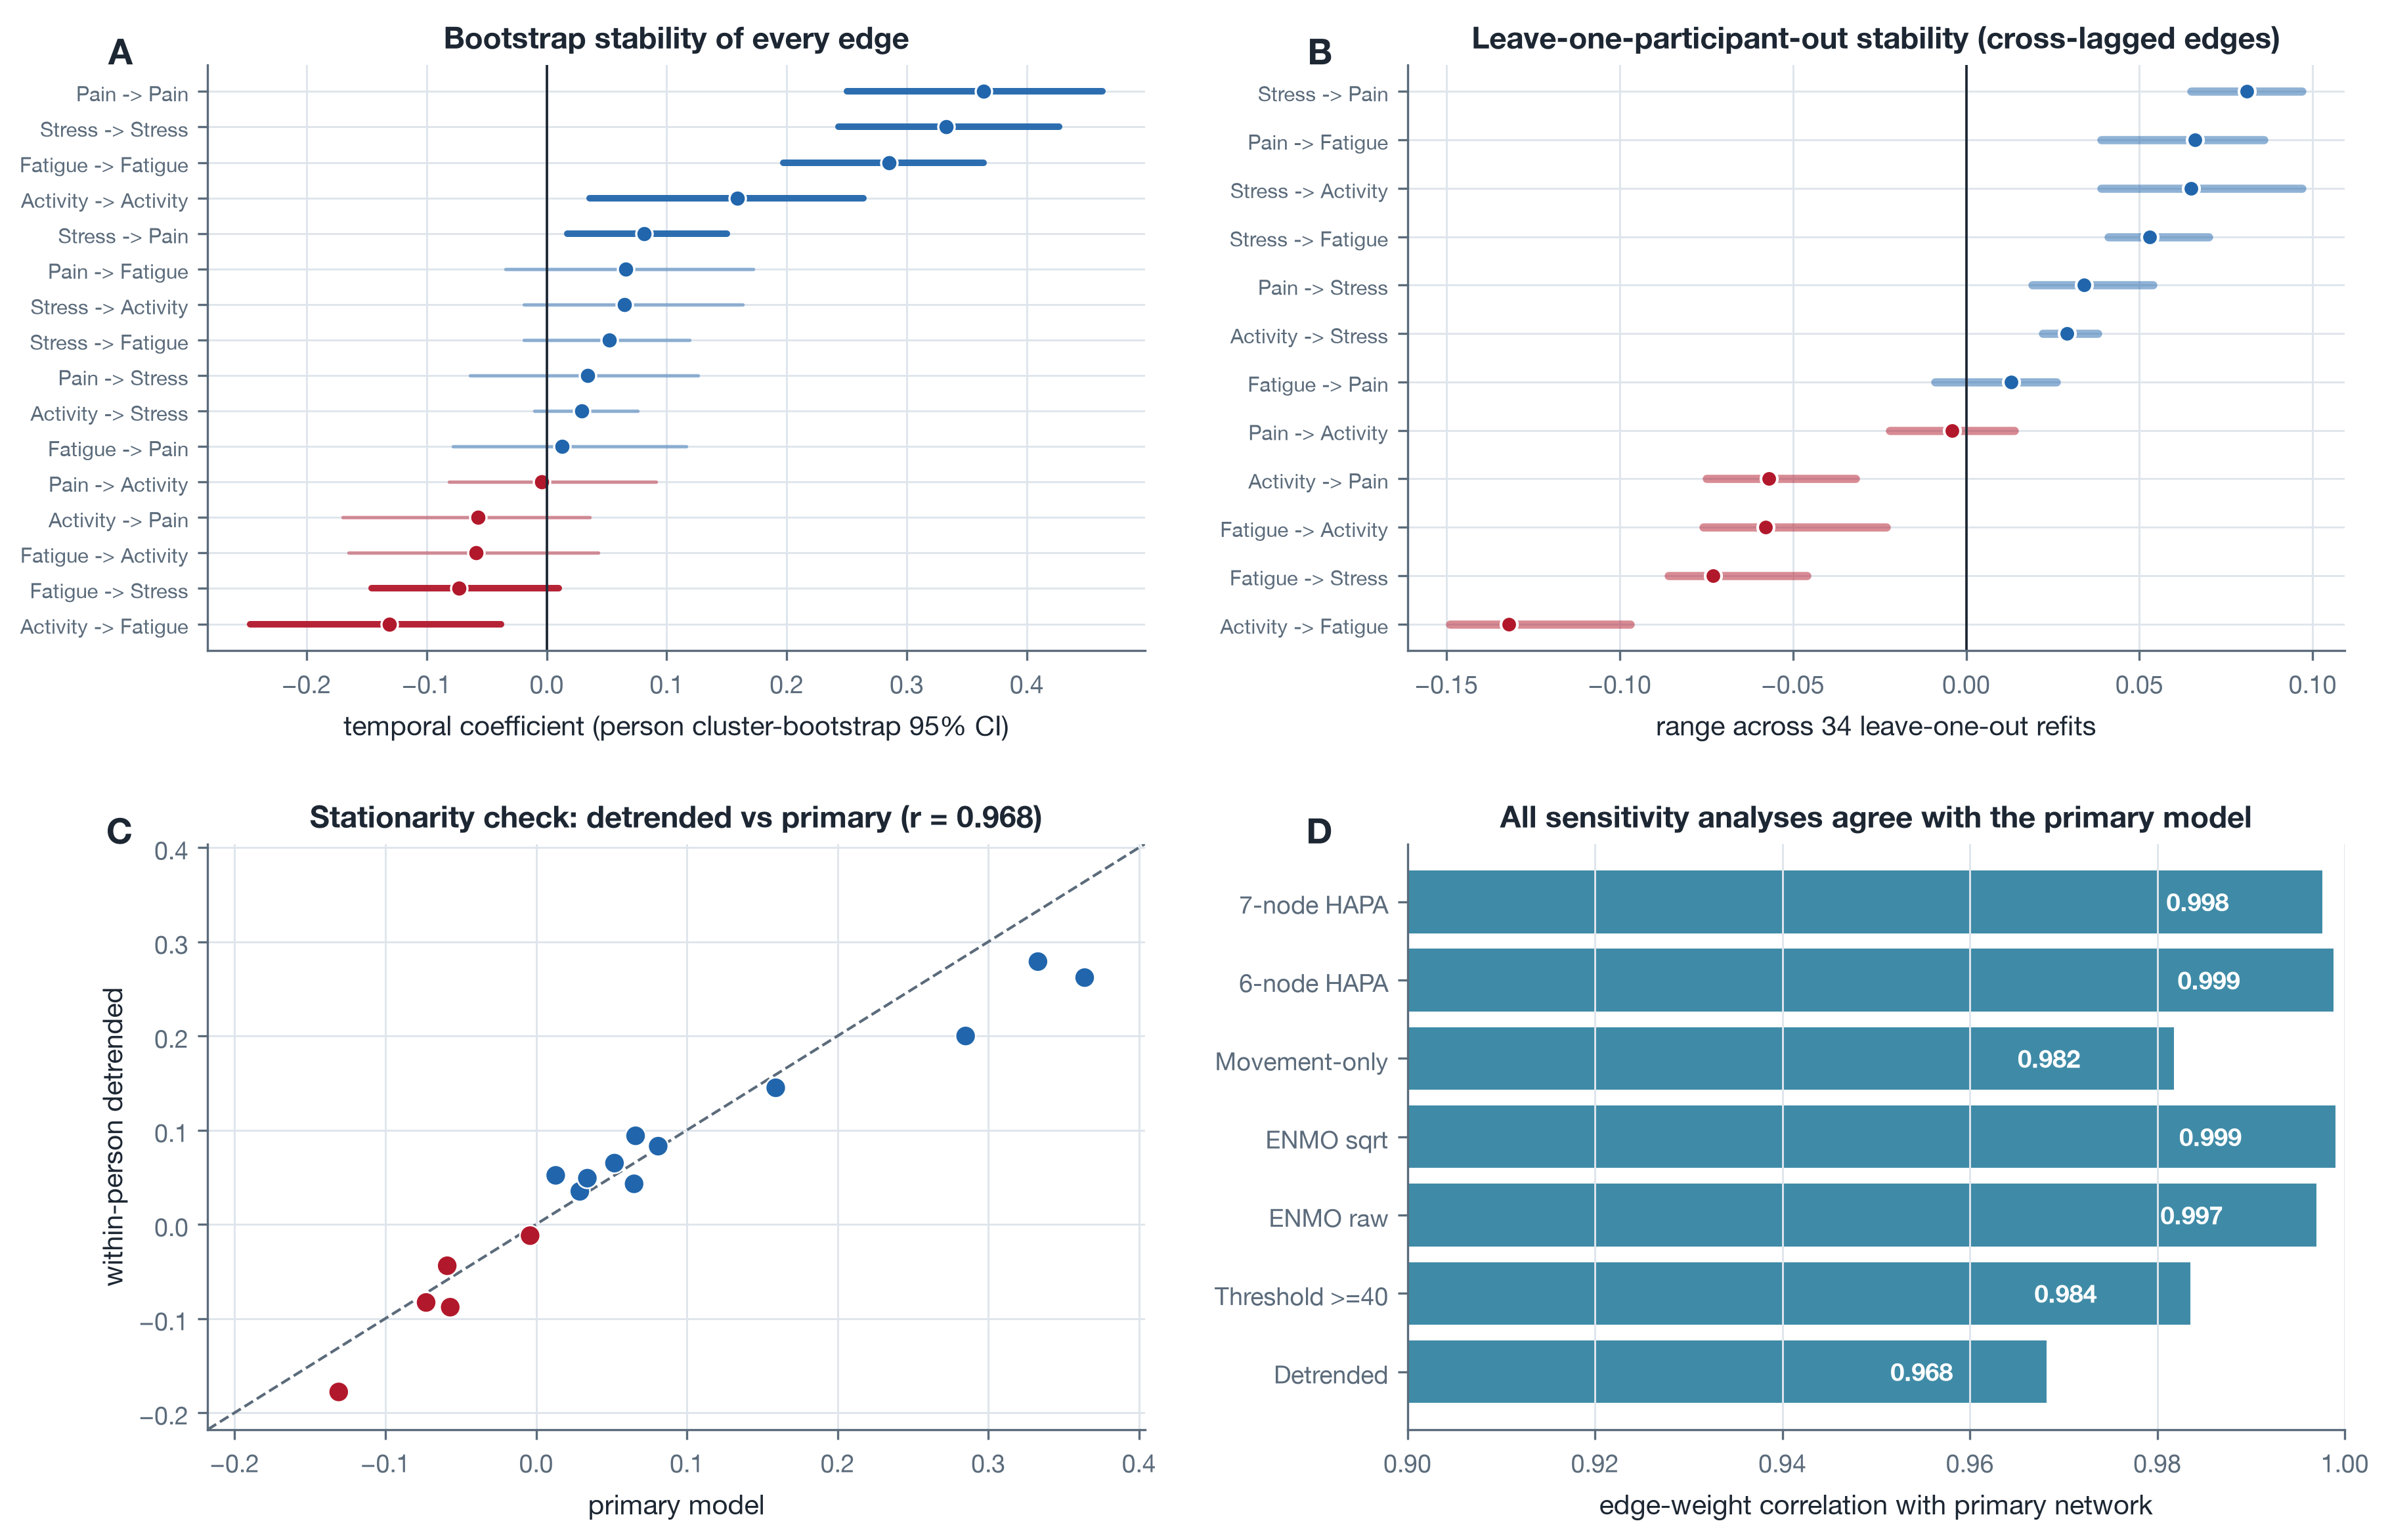
\includegraphics[width=0.92\textwidth]{../assets/figures/supplementary/SUP_12_robustness.png}
\figurenote{Panel A shows person cluster-bootstrap 95\% intervals for every temporal edge.
Panel B shows leave-one-participant-out ranges for the cross-lagged edges. Panel C compares
within-person detrended coefficients with the primary coefficients. Panel D shows the
edge-weight correlation of each sensitivity refit with the primary network.}
\end{figure}

\begin{figure}[H]
\raggedright
\caption{mlVAR residual diagnostics.}
\label{sfig:diagnostics}
\noindent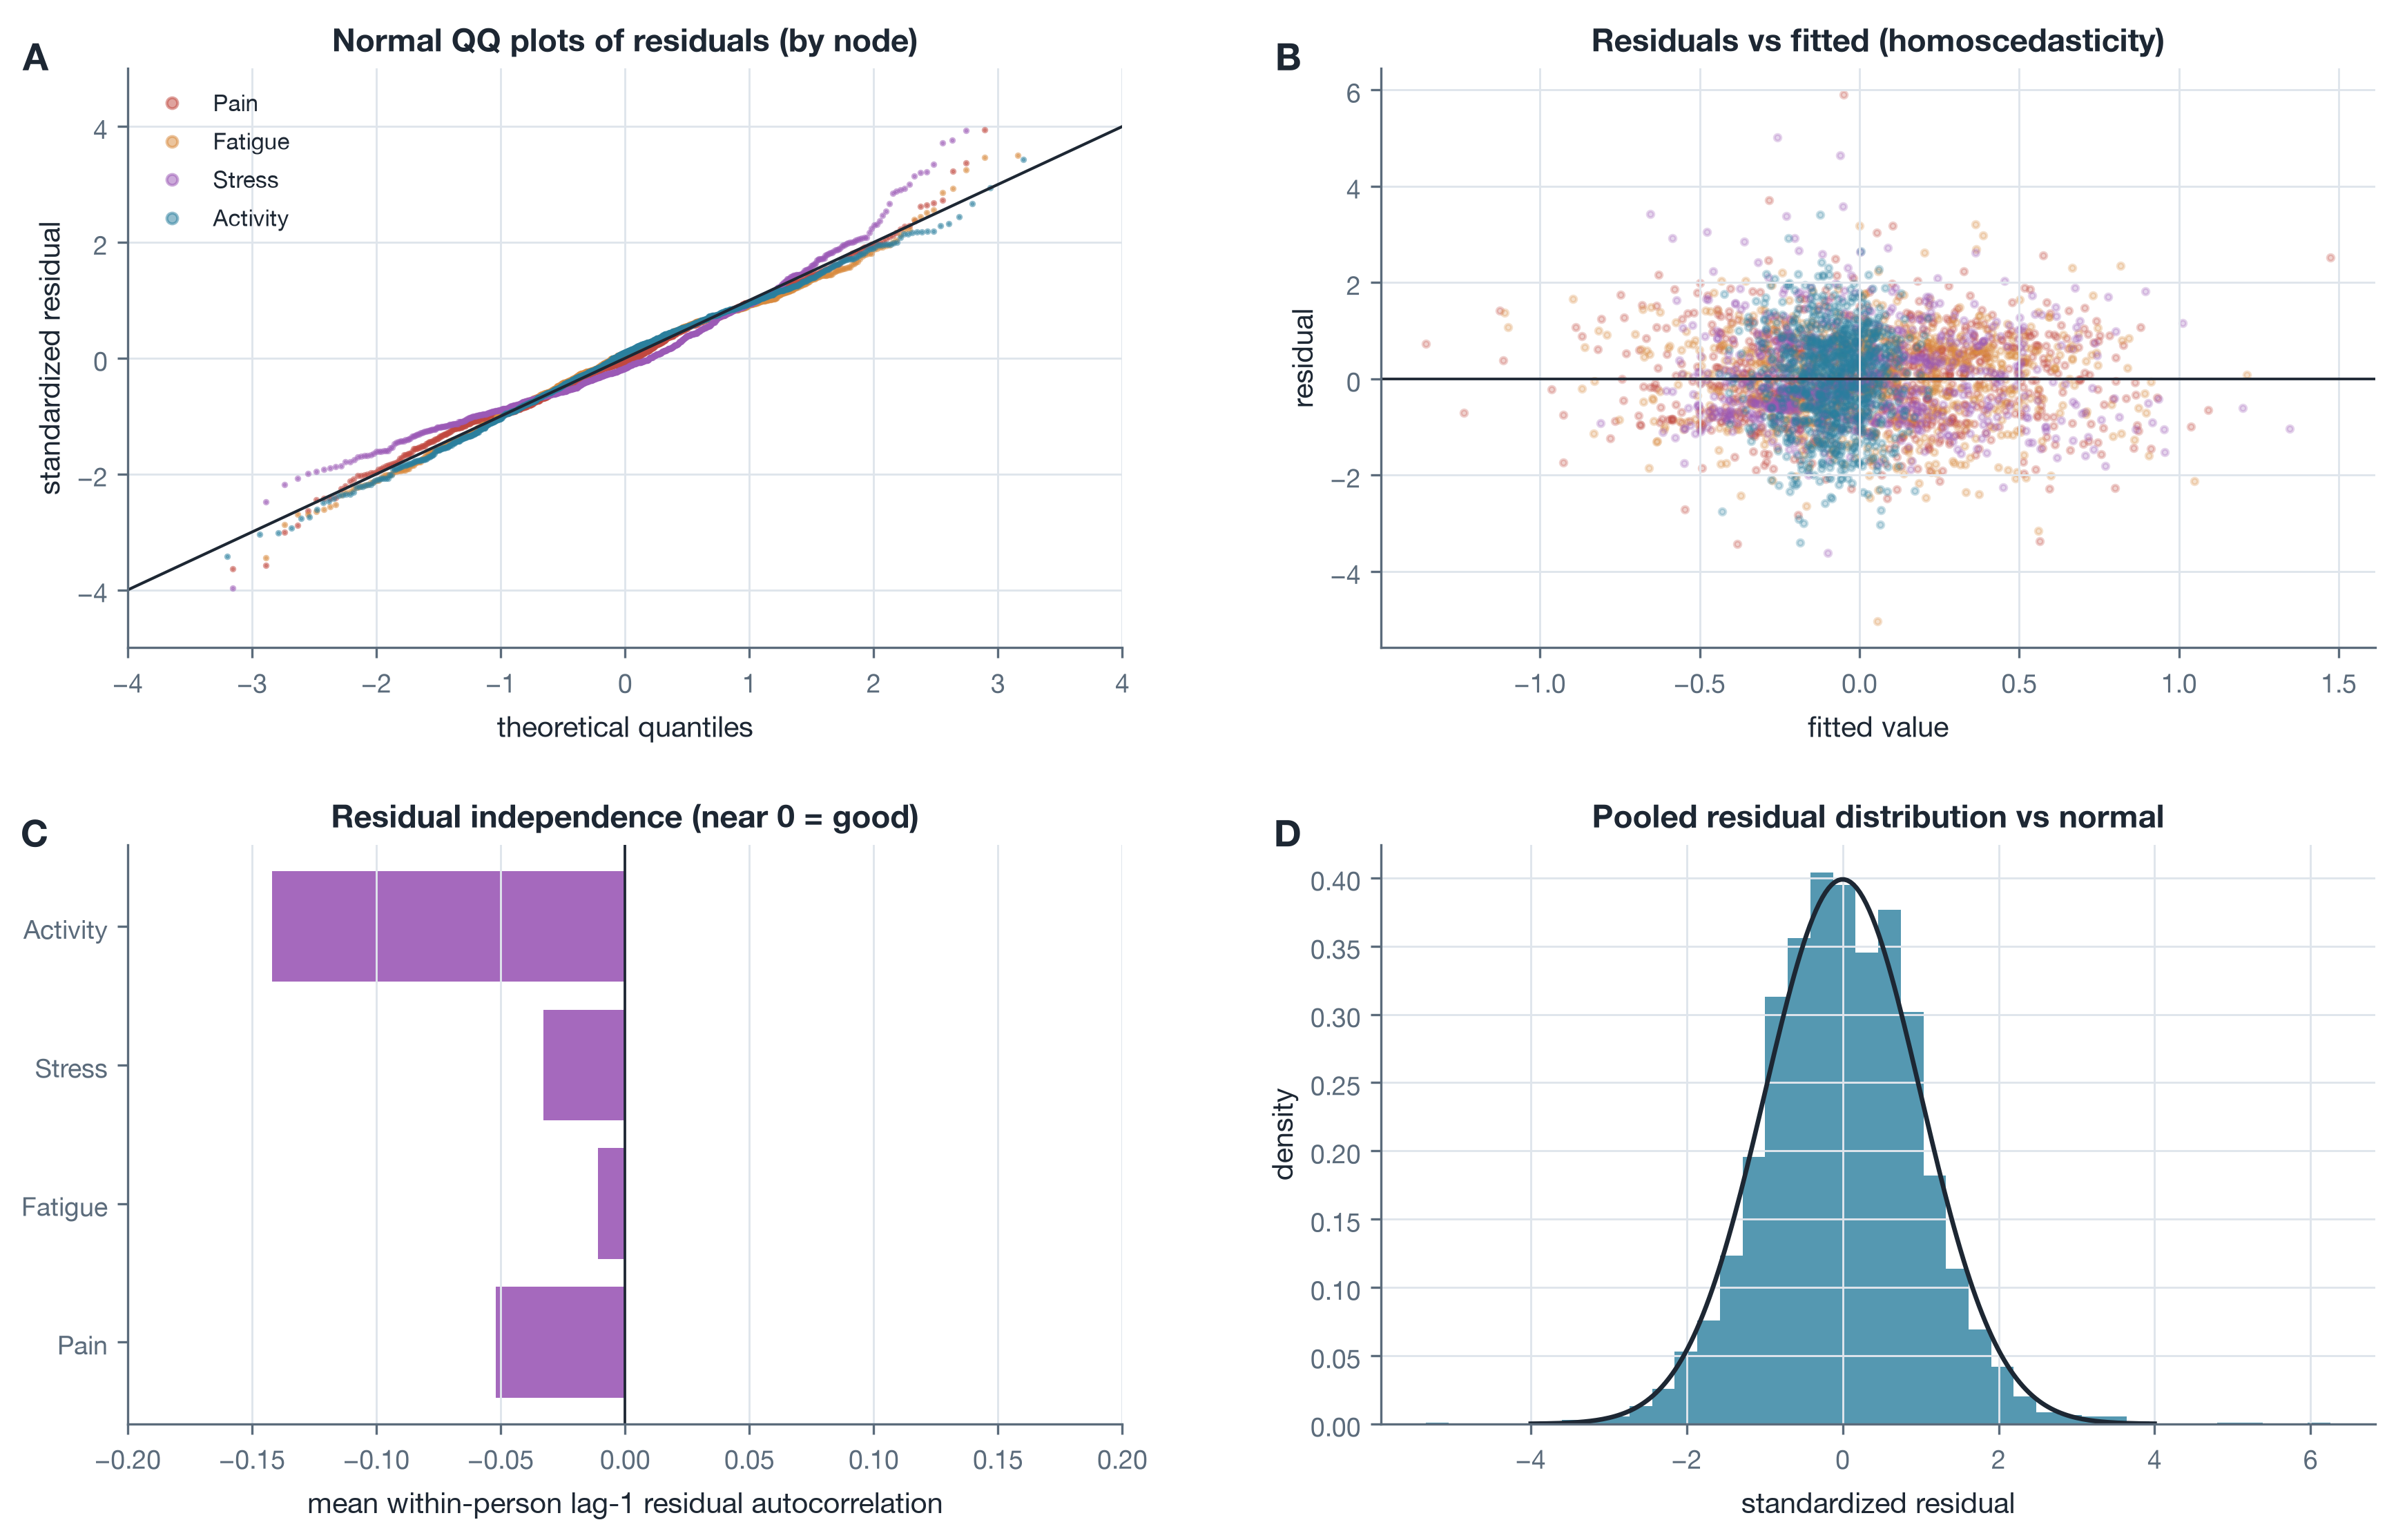
\includegraphics[width=0.92\textwidth]{../assets/figures/supplementary/SUP_13_model_diagnostics.png}
\figurenote{Panel A shows normal quantile plots of the residuals by node. Panel B shows
residuals versus fitted values. Panel C shows the mean within-person lag-1 residual
autocorrelation by node. Panel D shows the pooled residual distribution against a normal
density.}
\end{figure}

\begin{figure}[H]
\raggedright
\caption{Everyday context.}
\label{sfig:context}
\noindent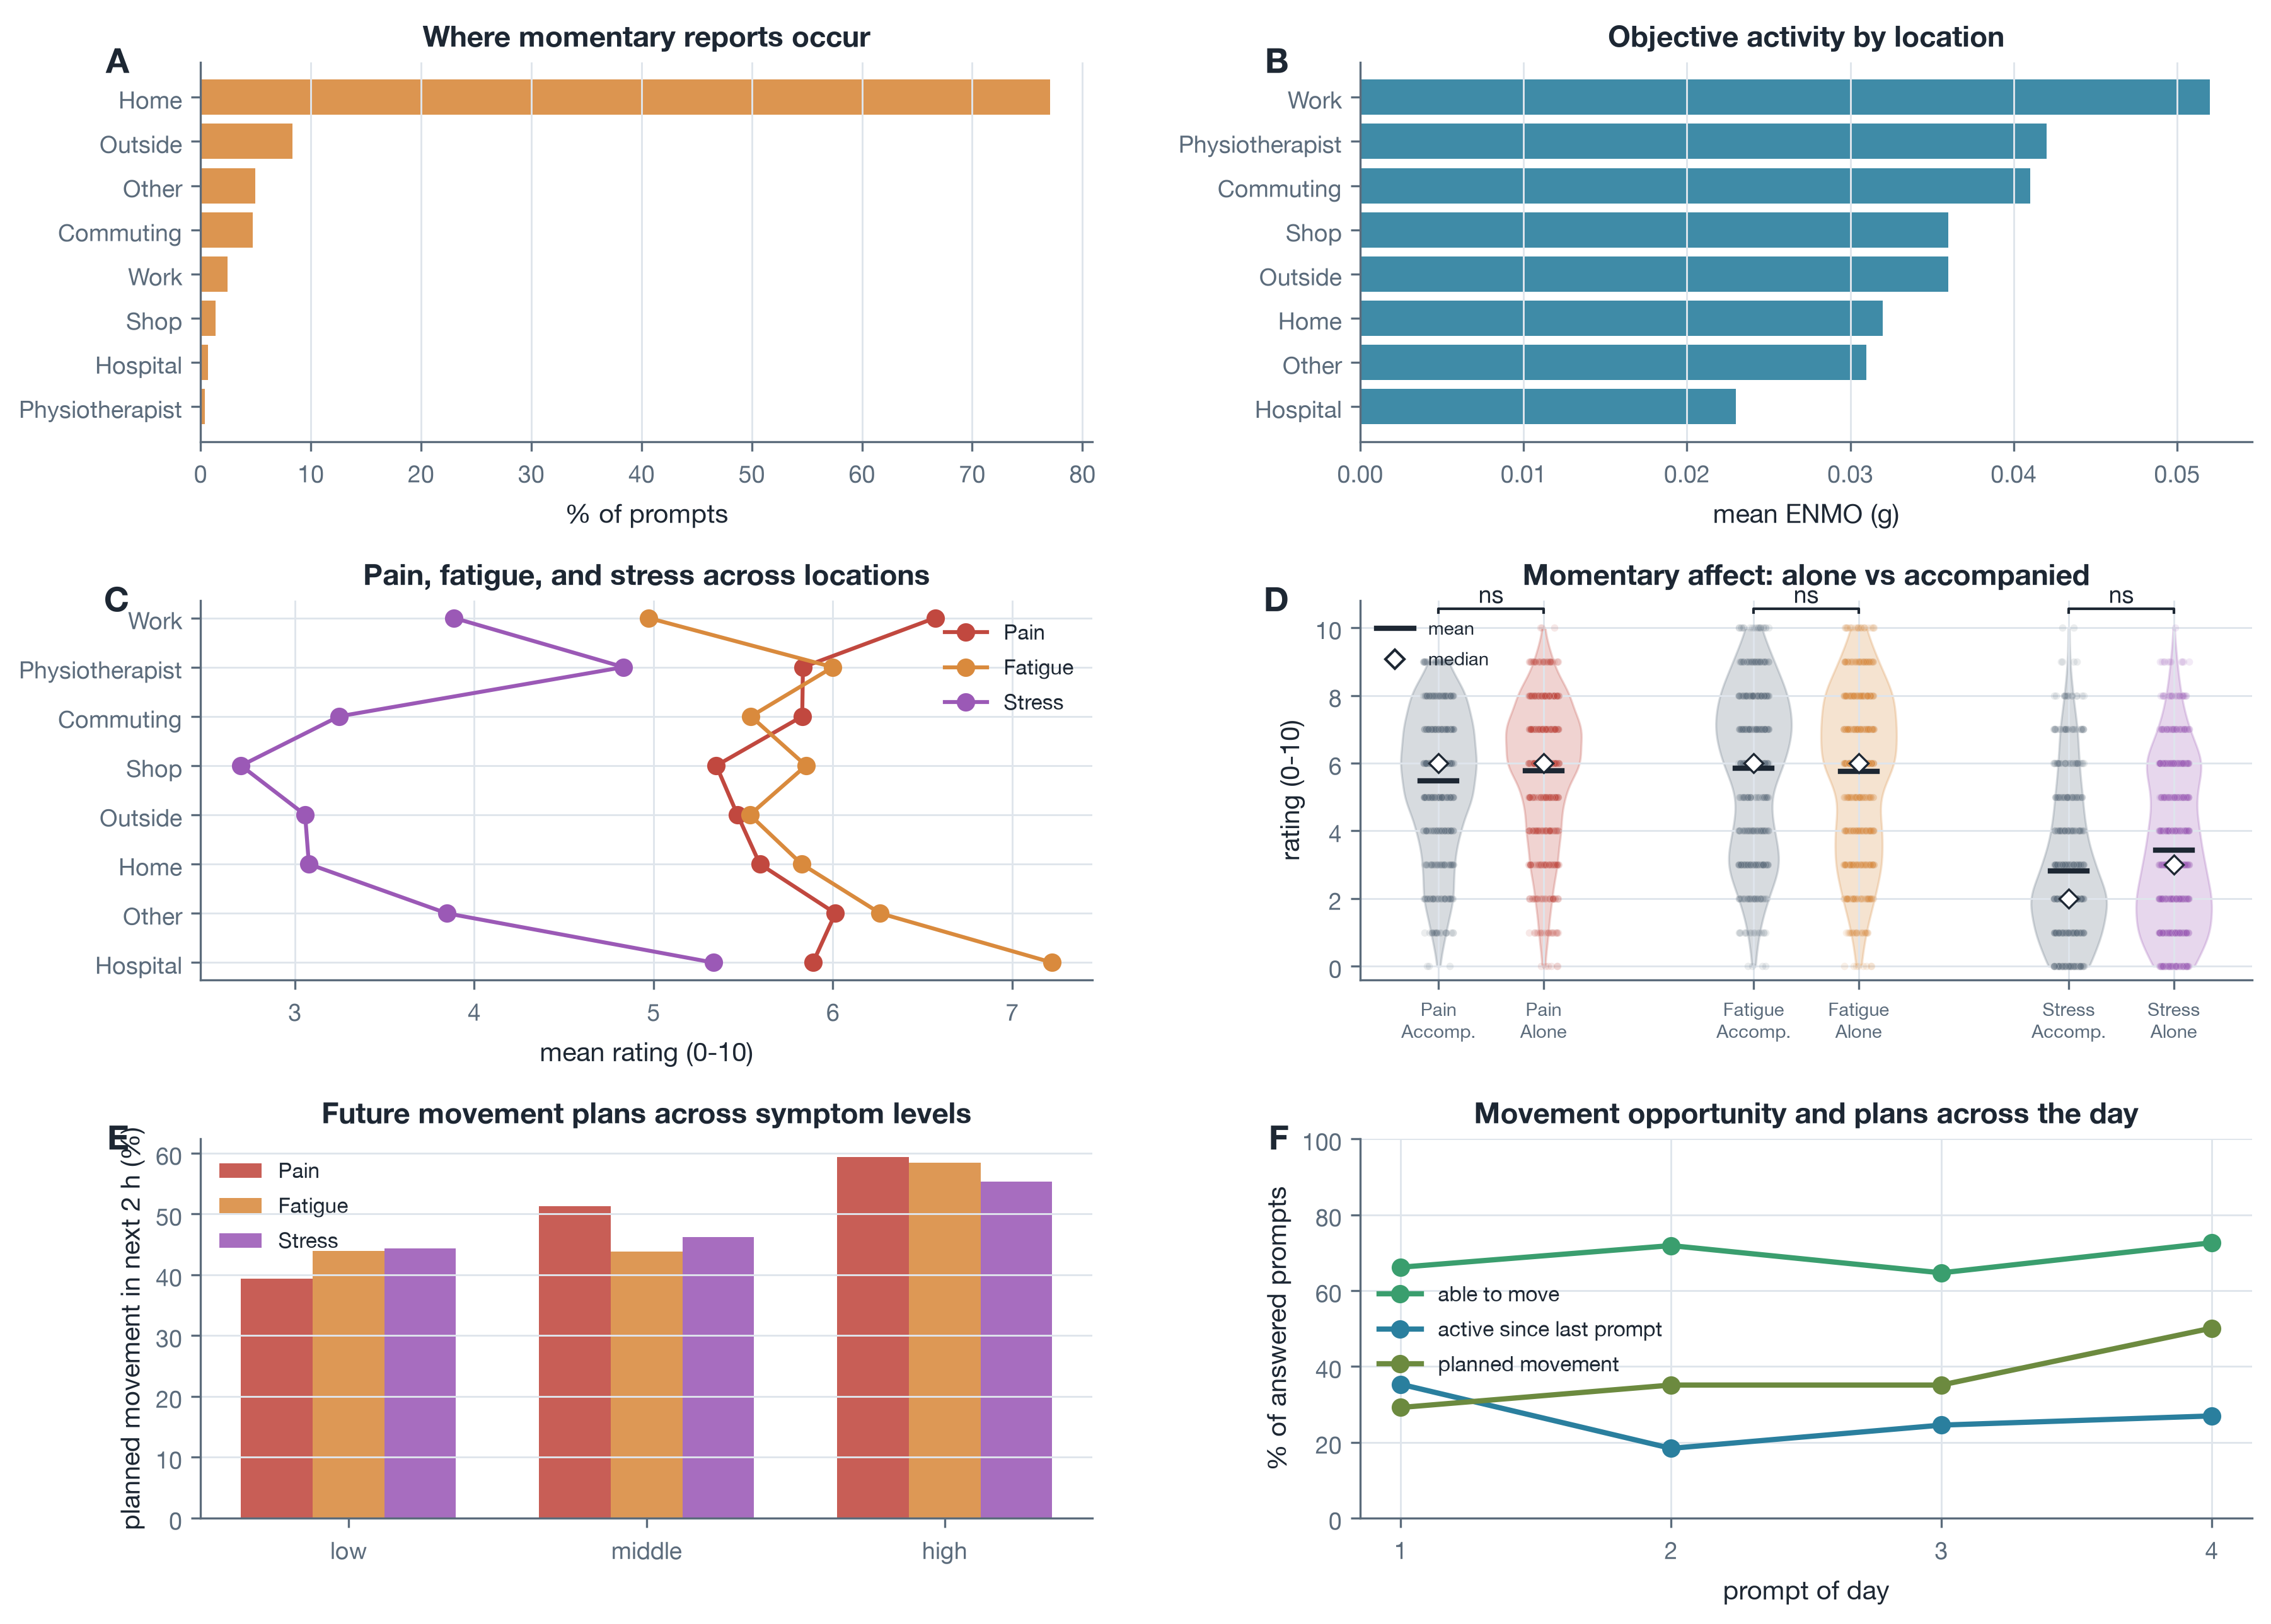
\includegraphics[width=0.92\textwidth]{../assets/figures/supplementary/SUP_14_context.png}
\figurenote{Panel A shows where prompts occurred. Panel B summarizes objective activity by
location. Panel C compares pain, fatigue, and stress across locations. Panel D compares pain,
fatigue, and stress when participants were alone versus accompanied using raw prompt-level
distributions, means, medians, and Gaussian GEE significance bars. Panel E
shows planned movement across symptom tertiles. Panel F shows movement opportunity, recent
activity, and planned movement across the four daily prompts.}
\end{figure}

\begin{figure}[H]
\raggedright
\caption{Weekday versus weekend day-type effects.}
\label{sfig:daytype}
\noindent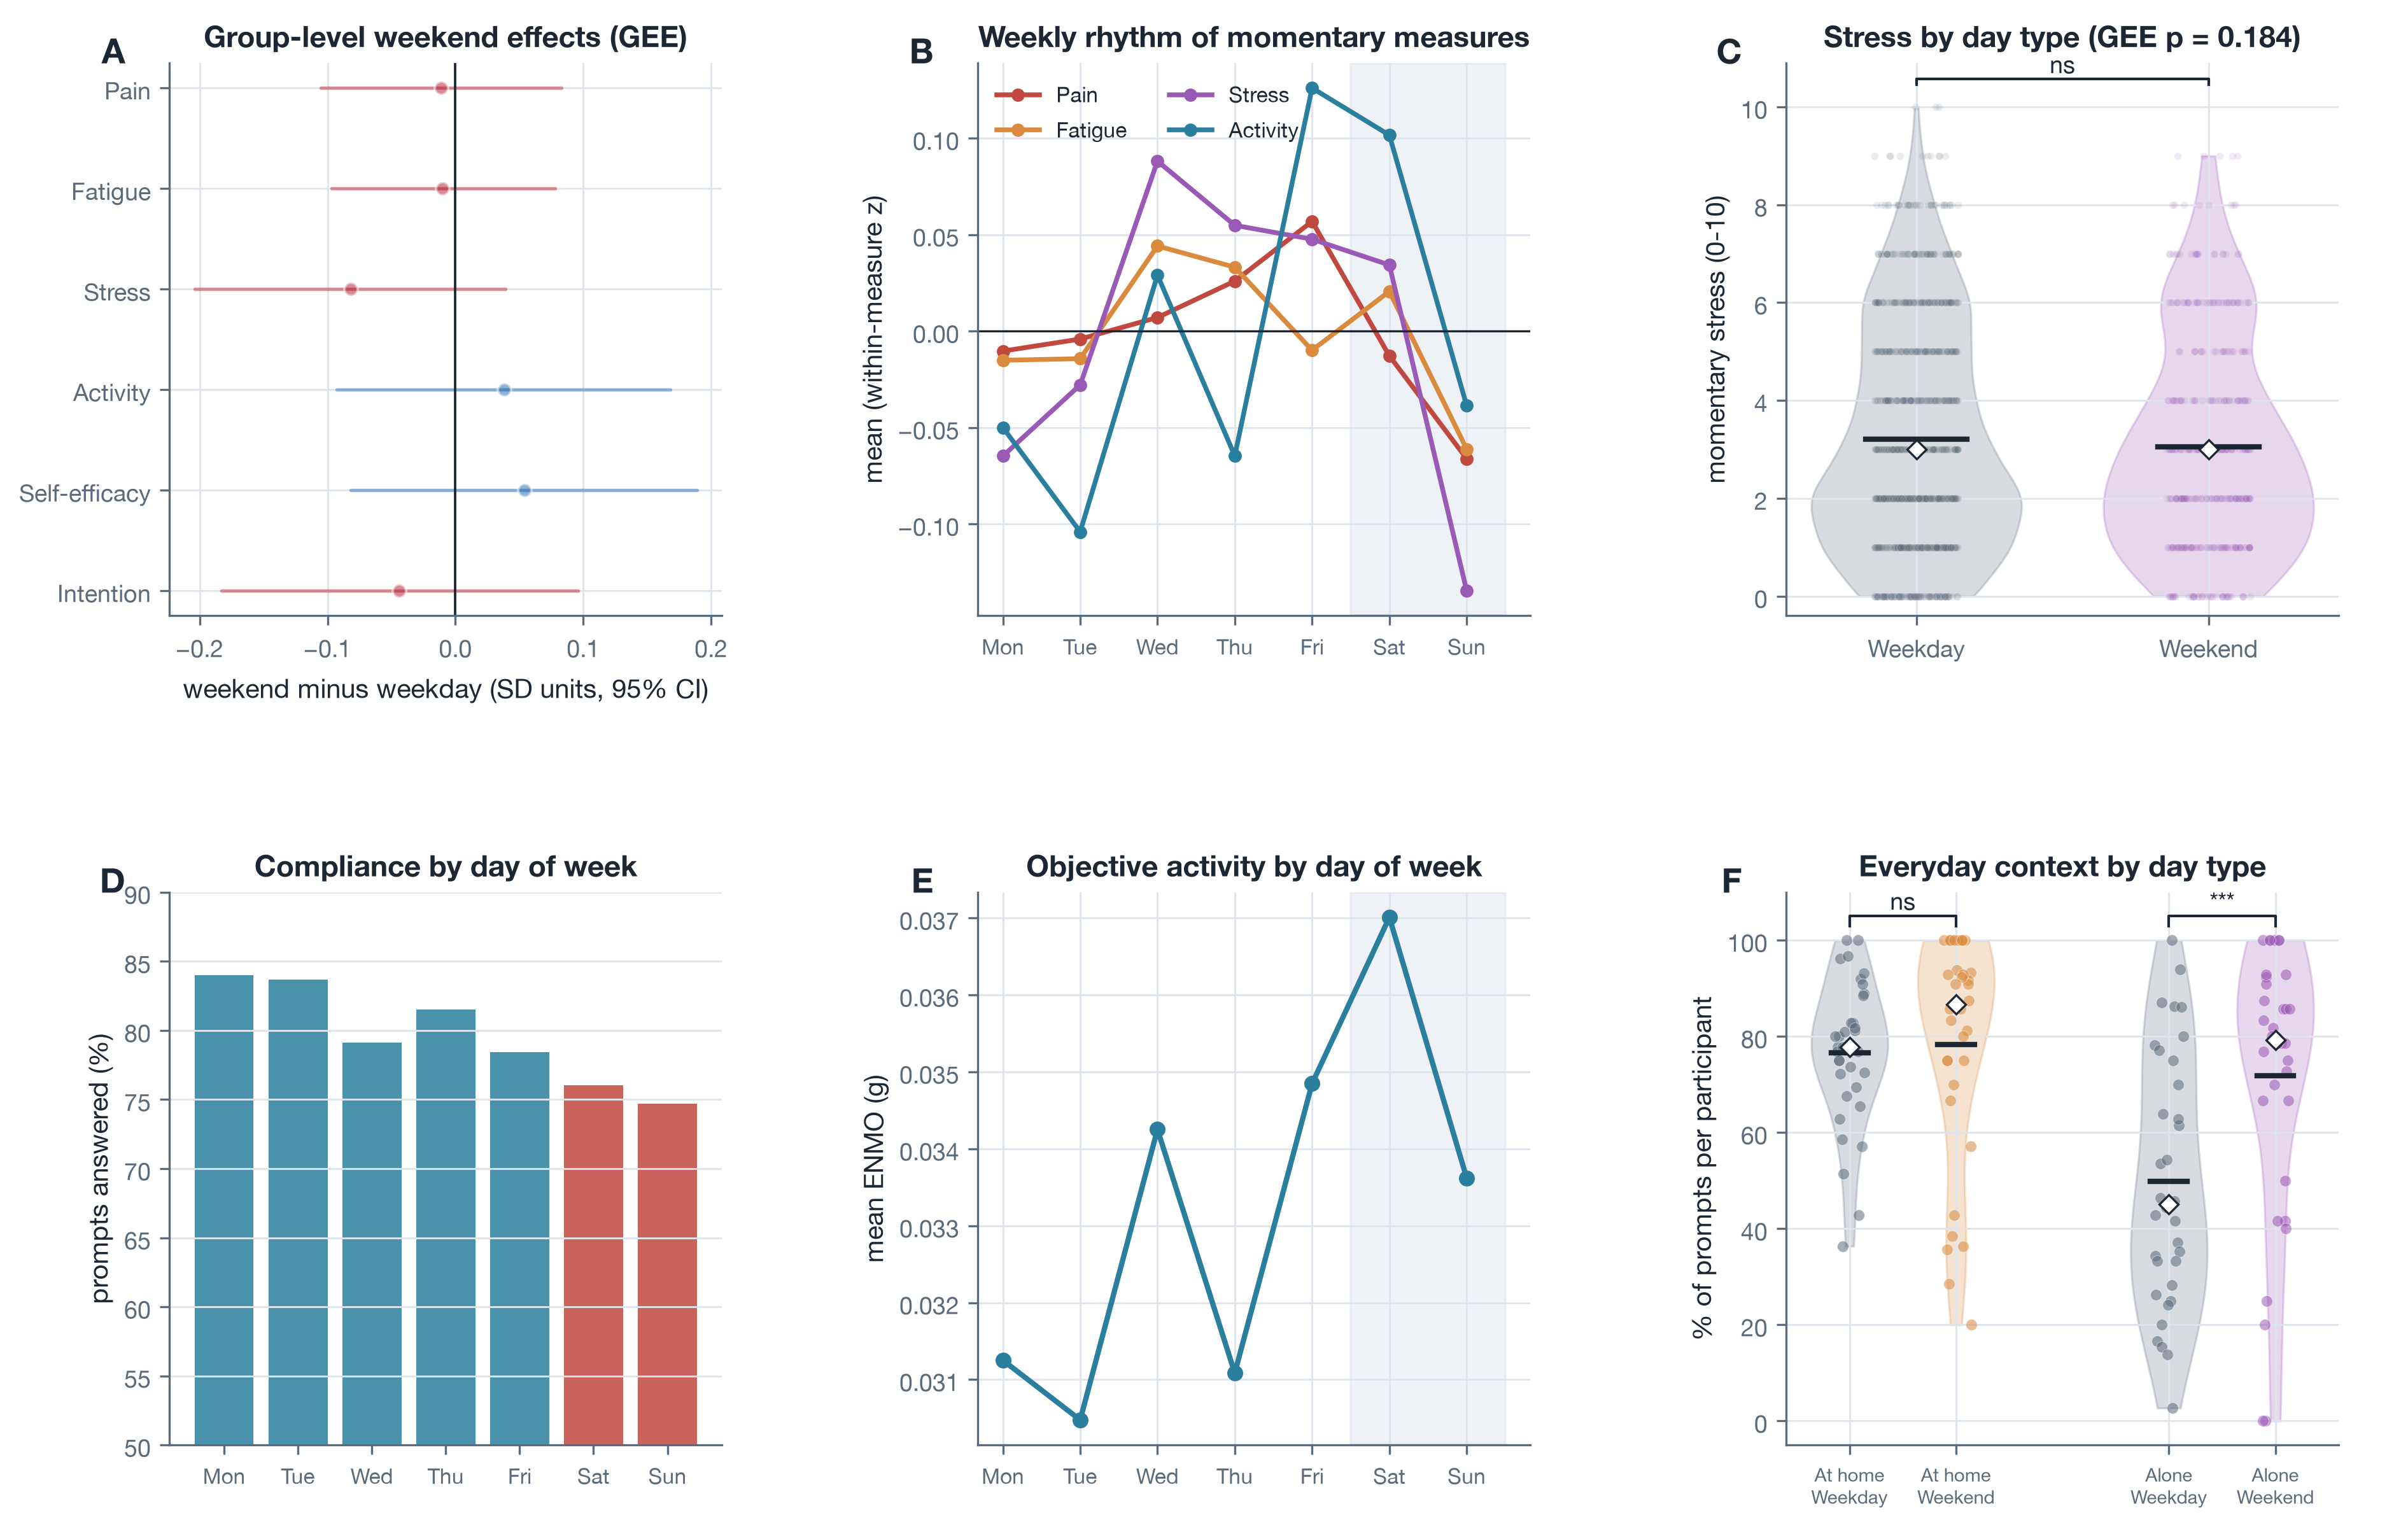
\includegraphics[width=0.92\textwidth]{../assets/figures/supplementary/SUP_15_daytype.png}
\figurenote{Day-type contrasts are estimated at the group level because individual weekday and
weekend series are short. Panel A shows the weekend-minus-weekday difference for each measure
in standard-deviation units with 95\% confidence intervals from Gaussian GEE models with
participant clustering. Panel B shows the weekly rhythm of the four core measures
(within-measure z-scores by day of week, weekend shaded). Panel C contrasts momentary stress
on weekdays and weekends using raw prompt-level distributions, means, medians, and the
Gaussian GEE significance bar. Panel D shows compliance by day of week. Panel E shows
objective activity by day of week. Panel F shows participant-level weekday and weekend
percentages for prompts at home and alone, with paired Wilcoxon significance bars.}
\end{figure}

\clearpage
\subsection*{Supplementary Tables}
\addcontentsline{toc}{subsection}{Supplementary Tables}

\begin{table}[H]
\raggedright
\caption{Contemporaneous and between-person networks.}
\label{tab:sup-contemporaneous-between}
\footnotesize
\begingroup
\setlength{\tabcolsep}{4pt}
\renewcommand{\arraystretch}{1.08}
\noindent
\begin{tabular*}{\textwidth}{@{\extracolsep{\fill}}llcc@{}}
\toprule
Network & Edge & Partial $r$ & $p$ \\
\midrule
Contemporaneous & Fatigue - Pain & 0.373 & <.001 \\
Contemporaneous & Stress - Pain & 0.19 & <.001 \\
Contemporaneous & Stress - Fatigue & 0.109 & .007 \\
Contemporaneous & Activity - Pain & -0.057 & .093 \\
Contemporaneous & Activity - Fatigue & -0.035 & .329 \\
Contemporaneous & Activity - Stress & 0.035 & .264 \\
Between-person & Fatigue - Pain & 0.716 & <.001 \\
Between-person & Stress - Pain & 0.175 & .304 \\
Between-person & Stress - Fatigue & 0.146 & .338 \\
Between-person & Activity - Pain & 0.072 & .551 \\
Between-person & Activity - Fatigue & -0.118 & .262 \\
Between-person & Activity - Stress & -0.217 & .133 \\
\bottomrule
\end{tabular*}
\par\vspace{3pt}\noindent\parbox{\textwidth}{\footnotesize\textit{Note.} Partial correlations from the primary mlVAR. The contemporaneous network represents same-prompt residual associations; the between-person network represents associations among person means.}
\endgroup
\end{table}

\begin{table}[H]
\raggedright
\caption{ENMO distribution and stationarity checks.}
\label{tab:sup-stationarity}
\footnotesize
\begingroup
\setlength{\tabcolsep}{4pt}
\renewcommand{\arraystretch}{1.08}
\noindent\textit{Panel A.} Skewness and kurtosis of candidate activity transformations.\par\vspace{2pt}
\begin{tabular*}{\textwidth}{@{\extracolsep{\fill}}lcc@{}}
\toprule
Measure & Skewness & Kurtosis \\
\midrule
ENMO (raw) & 1.321 & 5.403 \\
ENMO (sqrt) & 0.444 & 2.974 \\
ENMO (log) & -0.504 & 3.432 \\
\bottomrule
\end{tabular*}
\par\vspace{6pt}\noindent\textit{Panel B.} Share of individual series flagged by linear trend and KPSS diagnostics.\par\vspace{2pt}
\begin{tabular*}{\textwidth}{@{\extracolsep{\fill}}lcc@{}}
\toprule
Variable & Prop. linear trend & Prop. KPSS non-stationary \\
\midrule
Activity & 0.088 & 0.118 \\
Fatigue & 0.235 & 0.206 \\
Pain & 0.353 & 0.176 \\
Stress & 0.265 & 0.176 \\
\bottomrule
\end{tabular*}
\par\vspace{3pt}\noindent\parbox{\textwidth}{\footnotesize\textit{Note.} ENMO was analysed on the log scale because the transformed distribution was closest to symmetry. KPSS = Kwiatkowski-Phillips-Schmidt-Shin test.}
\endgroup
\end{table}

\begin{table}[H]
\raggedright
\caption{Missing data and imputation benchmark.}
\label{tab:sup-imputation}
\footnotesize
\begingroup
\setlength{\tabcolsep}{4pt}
\renewcommand{\arraystretch}{1.08}
\noindent\textit{Panel A.} Missingness by momentary measure (of 1,894 scheduled prompts).\par\vspace{2pt}
\begin{tabular*}{\textwidth}{@{\extracolsep{\fill}}lccc@{}}
\toprule
Measure & Observed & Missing & \% missing \\
\midrule
Pain & 1497 & 397 & 21.0 \\
Fatigue & 1495 & 399 & 21.1 \\
Stress & 1492 & 402 & 21.2 \\
Activity & 1757 & 137 & 7.2 \\
\bottomrule
\end{tabular*}
\par\vspace{6pt}\noindent\textit{Panel B.} Univariate and multivariate imputation compared by held-out reconstruction and moment stability.\par\vspace{2pt}
\begin{tabular*}{\textwidth}{@{\extracolsep{\fill}}llccccc@{}}
\toprule
Method & Type & Std. RMSE & Std. MAE & $r$ (held-out) & Mean shift (SD) & SD change (\%) \\
\midrule
Mean & Univariate & 1.021 & 0.801 & -0.286 & 0.014 & 3.6 \\
Median & Univariate & 1.067 & 0.771 & -0.064 & 0.026 & 2.4 \\
LOCF & Univariate & 1.321 & 0.961 & 0.117 & 0.011 & 1.6 \\
Linear interpolation & Univariate & 1.12 & 0.832 & 0.189 & 0.01 & 0.6 \\
Kalman (structural) & Univariate & 0.988 & 0.755 & 0.204 & 0.011 & 2.6 \\
KNN & Multivariate & 1.029 & 0.769 & 0.228 & 0.012 & 1.9 \\
MICE (chained eq.) & Multivariate & 0.954 & 0.73 & 0.321 & 0.012 & 3.2 \\
missForest (random forest) & Multivariate & 1.011 & 0.75 & 0.287 & 0.014 & 2.0 \\
\bottomrule
\end{tabular*}
\par\vspace{3pt}\noindent\parbox{\textwidth}{\footnotesize\textit{Note.} Symptom missingness reflects non-response; activity missingness reflects accelerometer non-wear. The primary analyses used available-case (pairwise) handling within each VAR equation, consistent with the missing-at-random evidence in the stationarity and missingness checks. As a sensitivity benchmark, 20\% of observed values were held out at random and reconstructed with five univariate imputeTS-style univariate time-series methods (Moritz \& Bartz-Beielstein, 2017) and three multivariate methods that borrow strength across the concurrent measures (k-nearest-neighbours, MICE with Bayesian ridge, and a random-forest chained imputer). Standardized RMSE, MAE, and the within-person held-out correlation are averaged over the four core measures; the last two columns give the change in each measure's pooled mean and SD after all gaps are imputed. Multivariate methods reconstructed momentary fluctuations best (MICE: RMSE = 0.95, $r$ = 0.32), the univariate mean and median did not track within-person fluctuations, and every method left the descriptive moments essentially unchanged, which supports the available-case decision. Figure S5 visualizes the full benchmark.}
\endgroup
\end{table}

\begin{table}[H]
\raggedright
\caption{S-GIMME path prevalence.}
\label{tab:sup-sgimme}
\scriptsize
\begingroup
\setlength{\tabcolsep}{4pt}
\renewcommand{\arraystretch}{1.08}
\noindent
\begin{tabular*}{\textwidth}{@{\extracolsep{\fill}}llccc@{}}
\toprule
Path & Path class & Group-level n & Individual n & Subgroup-1 n \\
\midrule
Activity $\leftarrow$ Activity(t-1) & Autoregressive & 30 & 0 & 0 \\
Fatigue $\leftarrow$ Fatigue(t-1) & Autoregressive & 30 & 0 & 0 \\
Pain $\leftarrow$ Pain(t-1) & Autoregressive & 30 & 0 & 0 \\
Stress $\leftarrow$ Stress(t-1) & Autoregressive & 30 & 0 & 0 \\
Fatigue $\leftarrow$ Pain & Cross-variable & 0 & 10 & 7 \\
Pain $\leftarrow$ Fatigue & Cross-variable & 0 & 5 & 0 \\
Pain $\leftarrow$ Stress & Cross-variable & 0 & 5 & 0 \\
Activity $\leftarrow$ Pain & Cross-variable & 0 & 4 & 0 \\
Fatigue $\leftarrow$ Stress(t-1) & Cross-variable & 0 & 4 & 0 \\
Stress $\leftarrow$ Pain & Cross-variable & 0 & 4 & 0 \\
Fatigue $\leftarrow$ Activity(t-1) & Cross-variable & 0 & 3 & 0 \\
Fatigue $\leftarrow$ Stress & Cross-variable & 0 & 3 & 0 \\
Pain $\leftarrow$ Fatigue(t-1) & Cross-variable & 0 & 3 & 0 \\
Pain $\leftarrow$ Stress(t-1) & Cross-variable & 0 & 3 & 0 \\
Stress $\leftarrow$ Fatigue & Cross-variable & 0 & 3 & 0 \\
Stress $\leftarrow$ Fatigue(t-1) & Cross-variable & 0 & 3 & 0 \\
Activity $\leftarrow$ Fatigue(t-1) & Cross-variable & 0 & 2 & 0 \\
Activity $\leftarrow$ Pain(t-1) & Cross-variable & 0 & 2 & 0 \\
Activity $\leftarrow$ Stress & Cross-variable & 0 & 2 & 0 \\
Fatigue $\leftarrow$ Pain(t-1) & Cross-variable & 0 & 2 & 0 \\
Stress $\leftarrow$ Activity & Cross-variable & 0 & 2 & 0 \\
Stress $\leftarrow$ Activity(t-1) & Cross-variable & 0 & 2 & 0 \\
Activity $\leftarrow$ Fatigue & Cross-variable & 0 & 1 & 0 \\
Activity $\leftarrow$ Stress(t-1) & Cross-variable & 0 & 1 & 0 \\
Pain $\leftarrow$ Activity & Cross-variable & 0 & 1 & 0 \\
Pain $\leftarrow$ Activity(t-1) & Cross-variable & 0 & 1 & 0 \\
\bottomrule
\end{tabular*}
\par\vspace{3pt}\noindent\parbox{\textwidth}{\scriptsize\textit{Note.} Counts are the number of participants for whom S-GIMME retained each path at the group, individual, or first subgroup level. The four autoregressive paths reached the group threshold; no cross-variable path reached that threshold. Path labels place the outcome on the left and the predictor on the right, with $(t-1)$ marking lagged terms. S-GIMME found 16 subgroups, including two small groups and 14 singletons.}
\endgroup
\end{table}

\begin{table}[H]
\raggedright
\caption{Per-person graphicalVAR feasibility.}
\label{tab:sup-graphicalvar}
\scriptsize
\begingroup
\setlength{\tabcolsep}{4pt}
\renewcommand{\arraystretch}{1.08}
\noindent
\begin{tabular*}{\textwidth}{@{\extracolsep{\fill}}lccccccc@{}}
\toprule
ID & Complete prompts & Fitted & Temporal edges & Contemp. edges & Temporal density & Pain $\rightarrow$ Activity & Activity $\rightarrow$ Pain \\
\midrule
P01 & 49 & yes & 0 & 2 & 0.0 & no & no \\
P02 & 33 & yes & 0 & 1 & 0.0 & no & no \\
P03 & 51 & yes & 2 & 0 & 0.125 & no & no \\
P04 & 49 & yes & 0 & 0 & 0.0 & no & no \\
P05 & 54 & yes & 0 & 1 & 0.0 & no & no \\
P06 & 47 & yes & 1 & 1 & 0.062 & no & no \\
P07 & 34 & yes & 0 & 0 & 0.0 & no & no \\
P08 & 17 & no & 0 & 0 & 0.0 & no & no \\
P09 & 28 & no & 0 & 0 & 0.0 & no & no \\
P10 & 45 & yes & 0 & 2 & 0.0 & no & no \\
P11 & 40 & yes & 0 & 1 & 0.0 & no & no \\
P12 & 43 & yes & 0 & 1 & 0.0 & no & no \\
P13 & 40 & yes & 0 & 0 & 0.0 & no & no \\
P14 & 36 & yes & 4 & 4 & 0.25 & no & no \\
P15 & 45 & yes & 3 & 1 & 0.188 & no & no \\
P16 & 23 & no & 0 & 0 & 0.0 & no & no \\
P17 & 45 & yes & 3 & 1 & 0.188 & no & no \\
P18 & 39 & yes & 6 & 1 & 0.375 & yes & no \\
P19 & 48 & yes & 9 & 0 & 0.562 & no & no \\
P20 & 39 & yes & 5 & 2 & 0.312 & no & no \\
P21 & 44 & yes & 0 & 0 & 0.0 & no & no \\
P22 & 37 & yes & 0 & 1 & 0.0 & no & no \\
P23 & 52 & yes & 2 & 2 & 0.125 & no & no \\
P24 & 49 & yes & 1 & 2 & 0.062 & no & no \\
P25 & 40 & yes & 3 & 0 & 0.188 & no & yes \\
P26 & 44 & yes & 4 & 0 & 0.25 & no & no \\
P27 & 46 & yes & 0 & 2 & 0.0 & no & no \\
P28 & 48 & yes & 0 & 2 & 0.0 & no & no \\
P29 & 39 & yes & 0 & 1 & 0.0 & no & no \\
P30 & 37 & yes & 0 & 0 & 0.0 & no & no \\
P31 & 24 & no & 0 & 0 & 0.0 & no & no \\
P32 & 50 & yes & 0 & 1 & 0.0 & no & no \\
P33 & 53 & yes & 6 & 0 & 0.375 & no & no \\
P34 & 41 & yes & 2 & 0 & 0.125 & no & yes \\
\bottomrule
\end{tabular*}
\par\vspace{3pt}\noindent\parbox{\textwidth}{\scriptsize\textit{Note.} Fully separate regularized individual networks were fitted with graphicalVAR and EBIC selection. Participants with fewer than 30 complete prompts were not fitted. Edge counts refer to nonzero selected edges in each person-specific network.}
\endgroup
\end{table}

\begin{table}[H]
\raggedright
\caption{Extended six-node model: temporal fixed effects.}
\label{tab:sup-extended}
\scriptsize
\begingroup
\setlength{\tabcolsep}{4pt}
\renewcommand{\arraystretch}{1.08}
\noindent
\begin{tabular*}{\textwidth}{@{\extracolsep{\fill}}lcccc@{}}
\toprule
Effect (lag-1) & Estimate & SE & $p$ & Random SD \\
\midrule
Activity $\rightarrow$ Self-efficacy & 0.276 & 0.066 & <.001 & 0.278 \\
Activity $\rightarrow$ Intention & 0.199 & 0.057 & .001 & 0.228 \\
Self-efficacy $\rightarrow$ Intention & -0.139 & 0.055 & .011 & 0.173 \\
Activity $\rightarrow$ Fatigue & -0.129 & 0.054 & .017 & 0.246 \\
Stress $\rightarrow$ Pain & 0.074 & 0.036 & .039 & 0.056 \\
Fatigue $\rightarrow$ Stress & -0.073 & 0.038 & .057 & 0.045 \\
Fatigue $\rightarrow$ Intention & -0.077 & 0.047 & .099 & 0.0 \\
Pain $\rightarrow$ Self-efficacy & -0.078 & 0.051 & .125 & 0.0 \\
Stress $\rightarrow$ Fatigue & 0.048 & 0.032 & .138 & 0.0 \\
Stress $\rightarrow$ Activity & 0.066 & 0.05 & .183 & 0.109 \\
Intention $\rightarrow$ Stress & -0.051 & 0.039 & .184 & 0.0 \\
Intention $\rightarrow$ Activity & 0.078 & 0.059 & .187 & 0.141 \\
Stress $\rightarrow$ Intention & 0.062 & 0.052 & .239 & 0.157 \\
Activity $\rightarrow$ Stress & 0.036 & 0.031 & .239 & 0.0 \\
Pain $\rightarrow$ Fatigue & 0.056 & 0.049 & .258 & 0.164 \\
Activity $\rightarrow$ Pain & -0.061 & 0.054 & .261 & 0.243 \\
Fatigue $\rightarrow$ Activity & -0.05 & 0.051 & .327 & 0.037 \\
Self-efficacy $\rightarrow$ Fatigue & -0.031 & 0.033 & .349 & 0.0 \\
Self-efficacy $\rightarrow$ Pain & -0.029 & 0.04 & .467 & 0.096 \\
Fatigue $\rightarrow$ Self-efficacy & -0.037 & 0.052 & .481 & 0.069 \\
Intention $\rightarrow$ Self-efficacy & 0.047 & 0.069 & .498 & 0.223 \\
Pain $\rightarrow$ Intention & -0.029 & 0.047 & .540 & 0.0 \\
Pain $\rightarrow$ Stress & 0.03 & 0.055 & .583 & 0.207 \\
Stress $\rightarrow$ Self-efficacy & 0.027 & 0.056 & .633 & 0.163 \\
Self-efficacy $\rightarrow$ Stress & 0.01 & 0.039 & .797 & 0.102 \\
Pain $\rightarrow$ Activity & 0.011 & 0.05 & .822 & 0.0 \\
Intention $\rightarrow$ Pain & 0.008 & 0.043 & .848 & 0.07 \\
Intention $\rightarrow$ Fatigue & -0.008 & 0.044 & .855 & 0.112 \\
Fatigue $\rightarrow$ Pain & 0.005 & 0.042 & .900 & 0.082 \\
Self-efficacy $\rightarrow$ Activity & 0.002 & 0.046 & .957 & 0.0 \\
Pain $\rightarrow$ Pain & 0.36 & 0.051 & <.001 & 0.172 \\
Fatigue $\rightarrow$ Fatigue & 0.284 & 0.04 & <.001 & 0.077 \\
Stress $\rightarrow$ Stress & 0.333 & 0.045 & <.001 & 0.158 \\
Intention $\rightarrow$ Intention & 0.325 & 0.062 & <.001 & 0.184 \\
Activity $\rightarrow$ Activity & 0.146 & 0.051 & .004 & 0.156 \\
Self-efficacy $\rightarrow$ Self-efficacy & 0.068 & 0.05 & .174 & 0.084 \\
\bottomrule
\end{tabular*}
\par\vspace{3pt}\noindent\parbox{\textwidth}{\scriptsize\textit{Note.} The model added momentary self-efficacy and intention. Core four-node edges correlated $r=.999$ with the primary model. Figure S8 also displays the corresponding seven-node extension that additionally includes rest-favouring outcome expectancy.}
\endgroup
\end{table}

\begin{table}[H]
\raggedright
\caption{Momentary pacing behaviour.}
\label{tab:sup-pacing}
\footnotesize
\begingroup
\setlength{\tabcolsep}{4pt}
\renewcommand{\arraystretch}{1.08}
\noindent\textit{Panel A.} Descriptives for momentary pacing items rated when participants had been active.\par\vspace{2pt}
\begin{tabular*}{\textwidth}{@{\extracolsep{\fill}}lrrrrrr@{}}
\toprule
item & n\_obs & mean & sd & median & min & max \\
\midrule
SPEED & 991 & 3.01 & 2.41 & 2 & 0 & 9 \\
PIECES & 991 & 3.07 & 2.45 & 3 & 0 & 9 \\
BREAKS & 989 & 2.95 & 2.48 & 2 & 0 & 10 \\
\bottomrule
\end{tabular*}
\par\vspace{6pt}\noindent\textit{Panel B.} Within-person symptoms predicting concurrent pacing.\par\vspace{2pt}
\begin{tabular*}{\textwidth}{@{\extracolsep{\fill}}lccc@{}}
\toprule
Predictor (within-person) & Estimate & SE & $p$ \\
\midrule
Pain & 0.129 & 0.039 & .001 \\
Fatigue & 0.122 & 0.035 & <.001 \\
Stress & -0.013 & 0.033 & .704 \\
\bottomrule
\end{tabular*}
\par\vspace{3pt}\noindent\parbox{\textwidth}{\footnotesize\textit{Note.} Pacing items were slowing down, breaking tasks into parts, and adding extra breaks. Estimates come from the multilevel model of symptom deviations on momentary pacing.}
\endgroup
\end{table}

\begin{table}[H]
\raggedright
\caption{Could-not-move sensitivity.}
\label{tab:sup-cantmove}
\footnotesize
\begingroup
\setlength{\tabcolsep}{4pt}
\renewcommand{\arraystretch}{1.08}
\noindent
\begin{tabular*}{\textwidth}{@{\extracolsep{\fill}}lccc@{}}
\toprule
Effect (lag-1) & All prompts & Movement-possible only & |difference| \\
\midrule
Stress $\rightarrow$ Fatigue & 0.052 & 0.115 & 0.063 \\
Fatigue $\rightarrow$ Fatigue & 0.285 & 0.239 & 0.046 \\
Stress $\rightarrow$ Pain & 0.081 & 0.117 & 0.036 \\
Stress $\rightarrow$ Stress & 0.333 & 0.367 & 0.034 \\
Fatigue $\rightarrow$ Activity & -0.059 & -0.027 & 0.032 \\
Stress $\rightarrow$ Activity & 0.065 & 0.035 & 0.03 \\
Fatigue $\rightarrow$ Stress & -0.073 & -0.099 & 0.026 \\
Pain $\rightarrow$ Activity & -0.004 & -0.025 & 0.021 \\
Pain $\rightarrow$ Fatigue & 0.066 & 0.084 & 0.018 \\
Activity $\rightarrow$ Fatigue & -0.131 & -0.118 & 0.013 \\
Pain $\rightarrow$ Pain & 0.364 & 0.375 & 0.011 \\
Fatigue $\rightarrow$ Pain & 0.013 & 0.004 & 0.009 \\
Activity $\rightarrow$ Activity & 0.159 & 0.164 & 0.005 \\
Activity $\rightarrow$ Pain & -0.057 & -0.053 & 0.004 \\
Pain $\rightarrow$ Stress & 0.034 & 0.036 & 0.002 \\
Activity $\rightarrow$ Stress & 0.029 & 0.03 & 0.001 \\
\bottomrule
\end{tabular*}
\par\vspace{3pt}\noindent\parbox{\textwidth}{\footnotesize\textit{Note.} Primary temporal coefficients were re-estimated after excluding prompts where movement was reported as impossible. Edge weights correlated $r=.982$ with the full model and no sign changes occurred.}
\endgroup
\end{table}

\begin{table}[H]
\raggedright
\caption{Stability of cross-lagged temporal edges: leave-one-participant-out and person cluster-bootstrap.}
\label{tab:robust}
\footnotesize
\begingroup
\setlength{\tabcolsep}{4pt}
\renewcommand{\arraystretch}{1.08}
\noindent
\begin{tabular*}{\textwidth}{@{\extracolsep{\fill}}lcccc@{}}
\toprule
Cross-lagged effect & Mean & LOPO range & Bootstrap 95\% CI & Bootstrap sign-consistency \\
\midrule
Activity $\rightarrow$ Fatigue & -0.132 & [-0.149, -0.097] & [-0.247, -0.038] & 0.994 \\
Fatigue $\rightarrow$ Stress & -0.073 & [-0.086, -0.046] & [-0.146, 0.010] & 0.956 \\
Fatigue $\rightarrow$ Activity & -0.058 & [-0.076, -0.023] & [-0.165, 0.043] & 0.858 \\
Activity $\rightarrow$ Pain & -0.057 & [-0.075, -0.032] & [-0.170, 0.036] & 0.878 \\
Pain $\rightarrow$ Activity & -0.004 & [-0.022, 0.014] & [-0.081, 0.091] & 0.526 \\
Fatigue $\rightarrow$ Pain & 0.013 & [-0.009, 0.026] & [-0.078, 0.116] & 0.618 \\
Activity $\rightarrow$ Stress & 0.029 & [0.022, 0.038] & [-0.010, 0.076] & 0.924 \\
Pain $\rightarrow$ Stress & 0.034 & [0.019, 0.054] & [-0.064, 0.126] & 0.746 \\
Stress $\rightarrow$ Fatigue & 0.053 & [0.041, 0.070] & [-0.019, 0.119] & 0.94 \\
Stress $\rightarrow$ Activity & 0.065 & [0.039, 0.097] & [-0.019, 0.163] & 0.936 \\
Pain $\rightarrow$ Fatigue & 0.066 & [0.039, 0.086] & [-0.034, 0.172] & 0.878 \\
Stress $\rightarrow$ Pain & 0.081 & [0.065, 0.097] & [0.017, 0.150] & 0.992 \\
\bottomrule
\end{tabular*}
\par\vspace{3pt}\noindent\parbox{\textwidth}{\footnotesize\textit{Note.} LOPO = 34 refits; bootstrap = 500 resamples. All cross-lagged edges retained their sign in 100\% of leave-one-out refits.}
\endgroup
\end{table}

\begin{table}[H]
\raggedright
\caption{Agreement of each sensitivity analysis with the primary temporal network.}
\label{tab:agreement}
\footnotesize
\begingroup
\setlength{\tabcolsep}{4pt}
\renewcommand{\arraystretch}{1.08}
\noindent
\begin{tabular*}{\textwidth}{@{\extracolsep{\fill}}lcc@{}}
\toprule
Sensitivity analysis & $r$ with primary & Sign flips \\
\midrule
Within-person detrended & 0.968 & 0 \\
Stricter compliance ($\geq 40$) & 0.984 & 0 \\
ENMO raw scale & 0.997 & 0 \\
ENMO square-root scale & 0.999 & 0 \\
Movement-possible only & 0.982 & 0 \\
Extended six-node model & 0.999 & 0 \\
Extended seven-node model & 0.998 & 0 \\
\bottomrule
\end{tabular*}
\par\vspace{3pt}\noindent\parbox{\textwidth}{\footnotesize\textit{Note.} $r$ = correlation of the 16 temporal coefficients with the primary model.}
\endgroup
\end{table}

\begin{table}[H]
\raggedright
\caption{Permutation inference for the network-POAM-P link.}
\label{tab:permutation}
\footnotesize
\begingroup
\setlength{\tabcolsep}{4pt}
\renewcommand{\arraystretch}{1.08}
\noindent
\begin{tabular*}{\textwidth}{@{\extracolsep{\fill}}lcccc@{}}
\toprule
Coupling & KW $H$ & Asymp. $p$ & Perm. $p$ & $n$ \\
\midrule
Pain $\rightarrow$ Activity & 6.46 & .040 & .037 & 30 \\
Activity $\rightarrow$ Pain & 4.149 & .126 & .128 & 27 \\
Activity $\rightarrow$ Fatigue & 4.215 & .121 & .119 & 27 \\
Stress $\rightarrow$ Activity & 1.646 & .439 & .456 & 30 \\
\bottomrule
\end{tabular*}
\par\vspace{3pt}\noindent\parbox{\textwidth}{\footnotesize\textit{Note.} Permutation tests used 10,000 label shuffles. The table reports Kruskal-Wallis tests of each coupling across POAM-P dominant patterns.}
\endgroup
\end{table}

\begin{table}[H]
\raggedright
\caption{Activity and affect by everyday context.}
\label{tab:sup-context}
\footnotesize
\begingroup
\setlength{\tabcolsep}{4pt}
\renewcommand{\arraystretch}{1.08}
\noindent\textit{Panel A.} Location-level summaries.\par\vspace{2pt}
\begin{tabular*}{\textwidth}{@{\extracolsep{\fill}}lcccccc@{}}
\toprule
Location & n prompts & \% prompts & Mean ENMO (g) & Mean pain & Mean fatigue & Mean stress \\
\midrule
Home & 1166 & 77.06 & 0.03 & 5.59 & 5.83 & 3.08 \\
Outside & 126 & 8.33 & 0.04 & 5.47 & 5.54 & 3.06 \\
Commuting & 72 & 4.76 & 0.04 & 5.83 & 5.54 & 3.25 \\
Work & 37 & 2.44 & 0.05 & 6.57 & 4.97 & 3.89 \\
Physiotherapist & 6 & 0.4 & 0.04 & 5.83 & 6.0 & 4.83 \\
Hospital & 10 & 0.66 & 0.02 & 5.89 & 7.22 & 5.33 \\
Shop & 21 & 1.39 & 0.04 & 5.35 & 5.85 & 2.7 \\
Other & 75 & 4.96 & 0.03 & 6.01 & 6.26 & 3.85 \\
\bottomrule
\end{tabular*}
\par\vspace{6pt}\noindent\textit{Panel B.} Social-context summaries.\par\vspace{2pt}
\begin{tabular*}{\textwidth}{@{\extracolsep{\fill}}lccccc@{}}
\toprule
Social context & n prompts & Mean ENMO (g) & Mean pain & Mean fatigue & Mean stress \\
\midrule
Accompanied & 680 & 0.03 & 5.47 & 5.85 & 2.82 \\
Alone & 827 & 0.03 & 5.77 & 5.76 & 3.43 \\
\bottomrule
\end{tabular*}
\par\vspace{6pt}\noindent\textit{Panel C.} Movement opportunity, recent activity, and plans by prompt of day.\par\vspace{2pt}
\begin{tabular*}{\textwidth}{@{\extracolsep{\fill}}lccc@{}}
\toprule
Prompt of day & Able to move (\%) & Active since last prompt (\%) & Planned movement (\%) \\
\midrule
1.0 & 66.2 & 35.3 & 29.2 \\
2.0 & 71.9 & 18.4 & 35.1 \\
3.0 & 64.7 & 24.5 & 35.1 \\
4.0 & 72.6 & 26.9 & 50.1 \\
\bottomrule
\end{tabular*}
\par\vspace{3pt}\noindent\parbox{\textwidth}{\footnotesize\textit{Note.} Context variables are descriptive. Able to move is based on the recoded movement-opportunity item, where 1 indicates that movement was possible.}
\endgroup
\end{table}

\begin{table}[H]
\raggedright
\caption{Primary four-node multilevel VAR temporal fixed effects.}
\label{tab:sup-temporal}
\footnotesize
\begingroup
\setlength{\tabcolsep}{4pt}
\renewcommand{\arraystretch}{1.08}
\noindent
\begin{tabular*}{\textwidth}{@{\extracolsep{\fill}}lccccc@{}}
\toprule
Effect (lag-1) & Estimate & SE & 95\% CI & $p$ & Random SD \\
\midrule
Activity $\rightarrow$ Fatigue & -0.131 & 0.054 & [-0.24, -0.03] & .015 & 0.249 \\
Stress $\rightarrow$ Pain & 0.081 & 0.036 & [0.01, 0.15] & .027 & 0.064 \\
Fatigue $\rightarrow$ Stress & -0.073 & 0.04 & [-0.15, 0.01] & .066 & 0.072 \\
Stress $\rightarrow$ Fatigue & 0.052 & 0.032 & [-0.01, 0.11] & .105 & 0.0 \\
Pain $\rightarrow$ Fatigue & 0.066 & 0.049 & [-0.03, 0.16] & .183 & 0.167 \\
Stress $\rightarrow$ Activity & 0.065 & 0.049 & [-0.03, 0.16] & .183 & 0.097 \\
Fatigue $\rightarrow$ Activity & -0.059 & 0.049 & [-0.16, 0.04] & .235 & 0.0 \\
Activity $\rightarrow$ Pain & -0.057 & 0.053 & [-0.16, 0.05] & .281 & 0.24 \\
Activity $\rightarrow$ Stress & 0.029 & 0.03 & [-0.03, 0.09] & .332 & 0.0 \\
Pain $\rightarrow$ Stress & 0.034 & 0.054 & [-0.07, 0.14] & .527 & 0.207 \\
Fatigue $\rightarrow$ Pain & 0.013 & 0.044 & [-0.07, 0.10] & .769 & 0.111 \\
Pain $\rightarrow$ Activity & -0.004 & 0.05 & [-0.10, 0.09] & .936 & 0.0 \\
Pain $\rightarrow$ Pain & 0.364 & 0.053 & [0.26, 0.47] & <.001 & 0.186 \\
Fatigue $\rightarrow$ Fatigue & 0.285 & 0.042 & [0.20, 0.37] & <.001 & 0.098 \\
Stress $\rightarrow$ Stress & 0.333 & 0.046 & [0.24, 0.42] & <.001 & 0.161 \\
Activity $\rightarrow$ Activity & 0.159 & 0.055 & [0.05, 0.27] & .004 & 0.2 \\
\bottomrule
\end{tabular*}
\par\vspace{3pt}\noindent\parbox{\textwidth}{\footnotesize\textit{Note.} This table repeats the primary temporal fixed-effect estimates for reference in the supplement. Standardized within-person coefficients are shown.}
\endgroup
\end{table}


\end{document}
